%\appendix
\chapter{Validation findings}

\section{Experience of validation group participants}

\section{Validation of antifragile attributes}


\newpage
\subsection{Optionality}
\begin{figure}[h!]
	\centering
	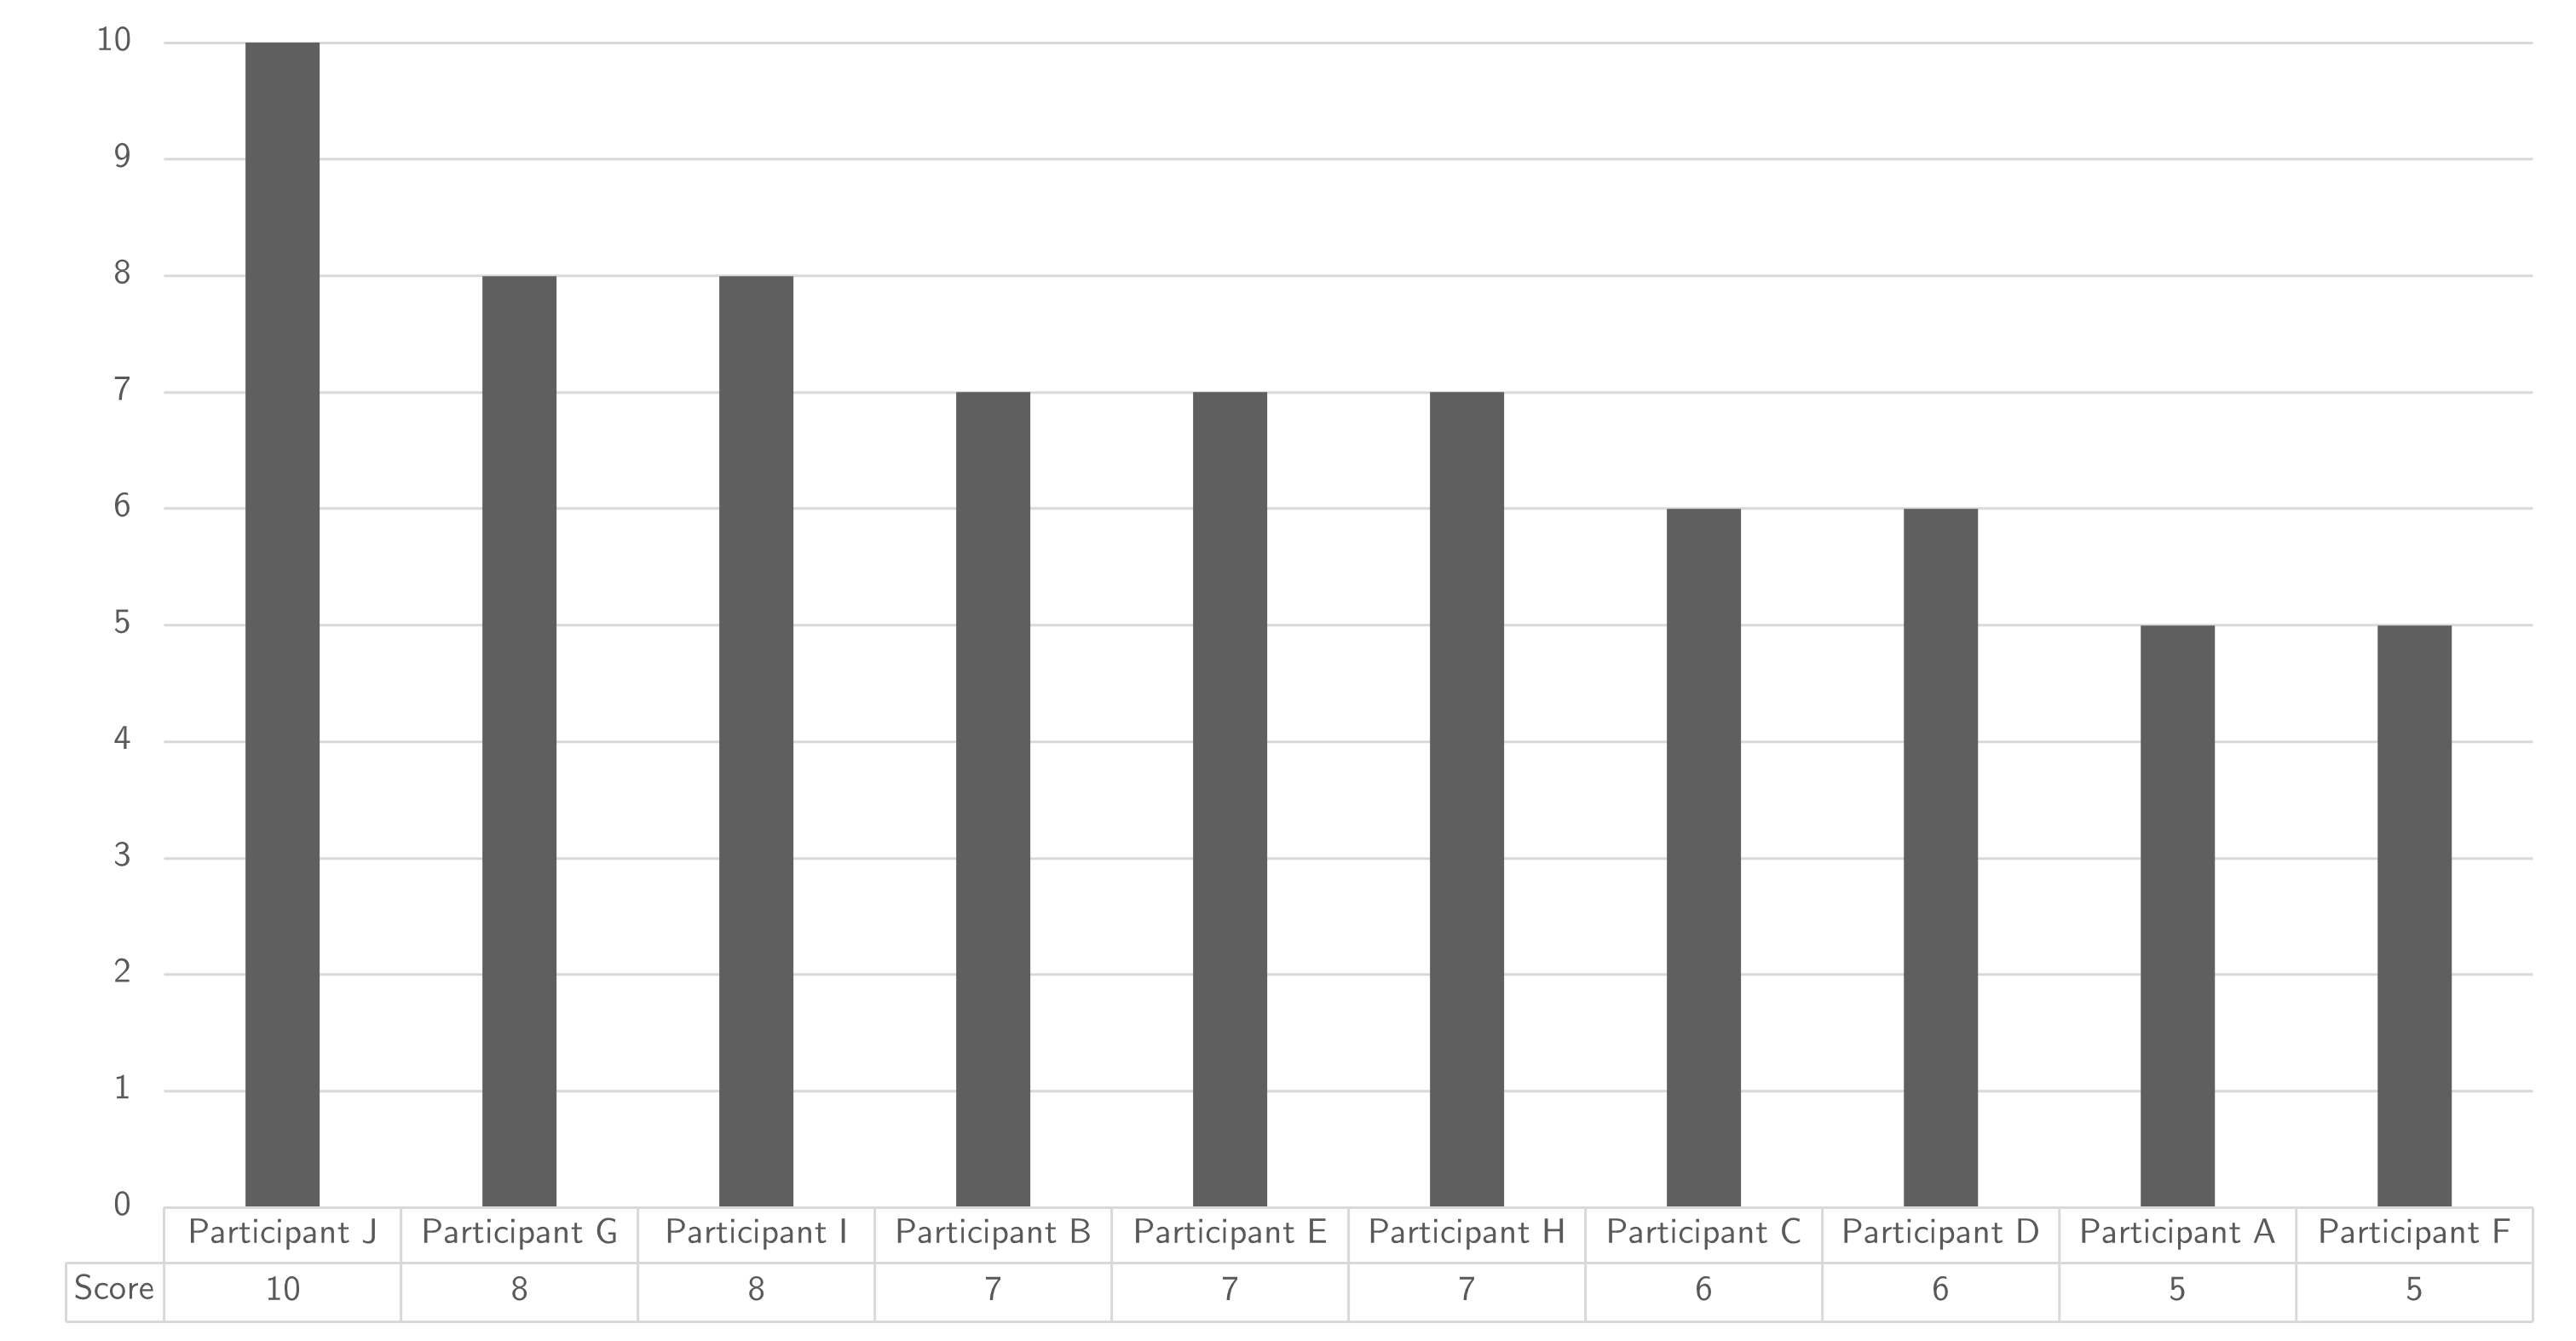
\includegraphics[width=0.9\linewidth]{images/scoreafoptionality}
	\caption[Scoring of antifragile attribute Optionality]{Scoring of antifragile attribute Optionality}
	\label{fig:appscoringafoptionality}
\end{figure}
\begin{table}[h!]
	\centering
	\begin{tabular}{p{.55\textwidth}ccc}
		\toprule
		\textbf{Attribute} & \textbf{Rating} & \textbf{Variability} & \textbf{Abstains} \\
		\midrule
		Optionality & 6,9 & 32\% & 0 \\%
		\bottomrule
	\end{tabular}%
	\caption[Scoring of antifragile attribute Optionality]{Scoring of antifragile attribute Optionality}
	\label{tab:appscoringafoptionality}%
\end{table}%
\newpage
\subsection{Mono-Monotonicity}
\begin{figure}[h!]
	\centering
	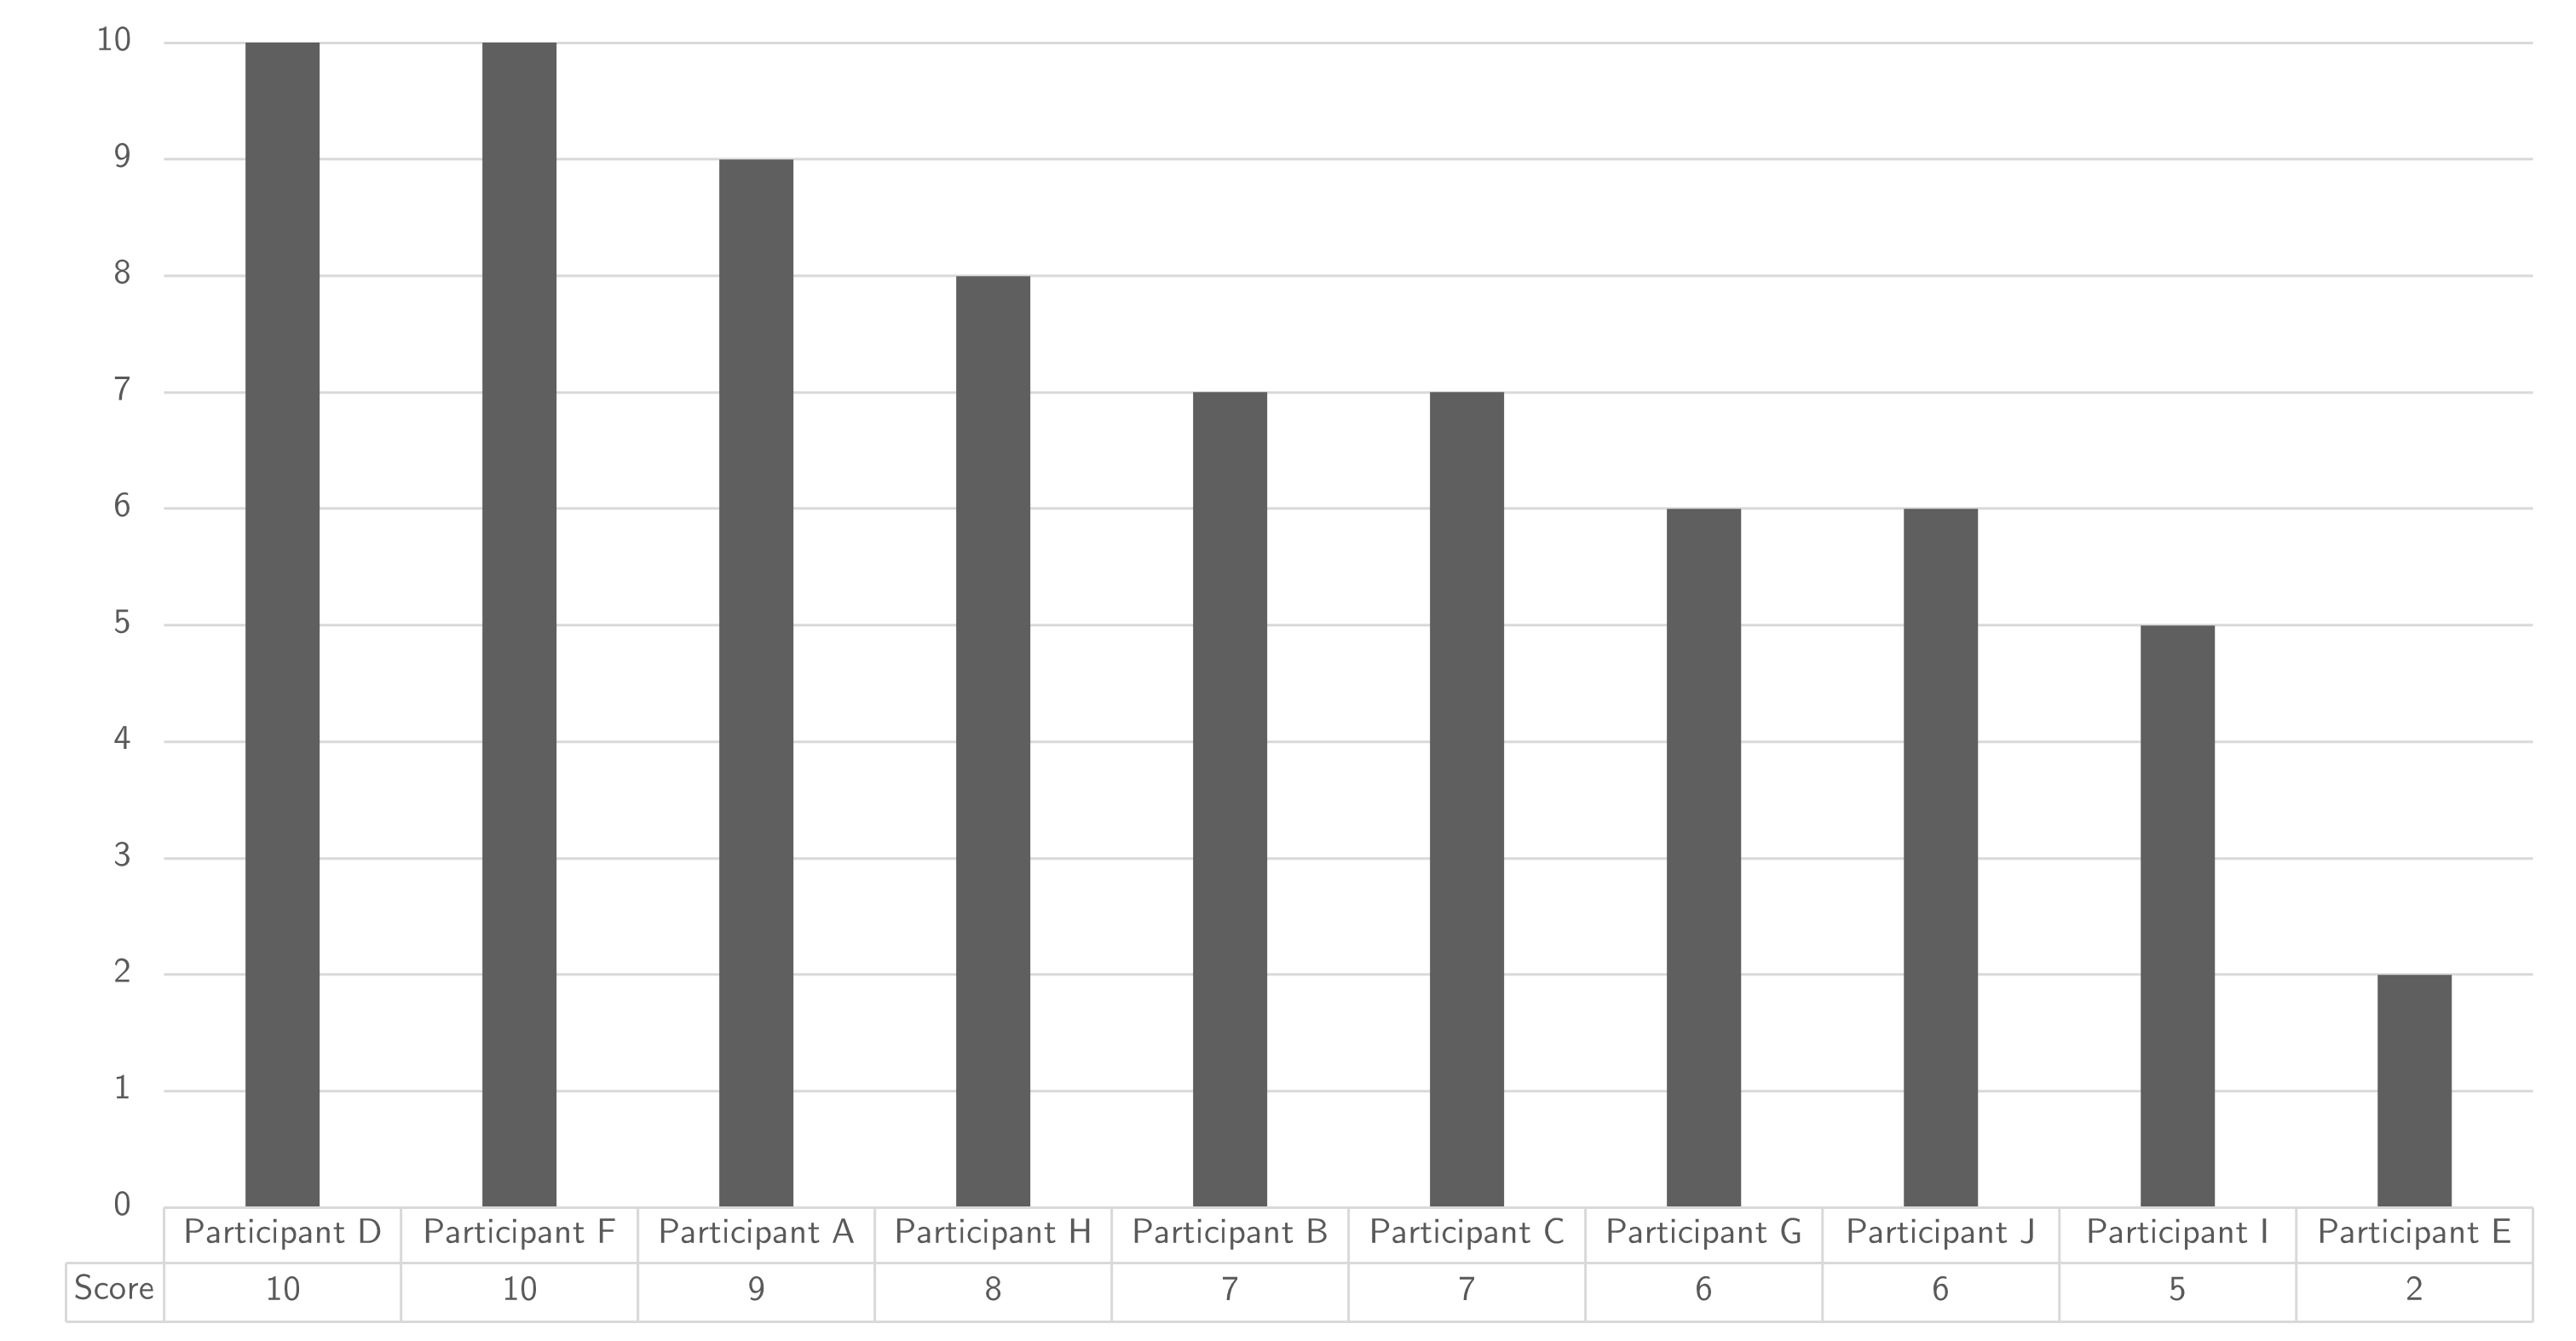
\includegraphics[width=0.9\linewidth]{images/scoreafmonomonotonicity}
	\caption[Scoring of antifragile attribute Mono-Monotonicity]{Scoring of antifragile attribute Mono-Monotonicity}
	\label{fig:appscoringafmonomonotonicity}
\end{figure}
\begin{table}[h!]
	\centering
	\begin{tabular}{p{.55\textwidth}ccc}
		\toprule
		\textbf{Attribute} & \textbf{Rating} & \textbf{Variability} & \textbf{Abstains} \\
		\midrule
		Mono-Monotonicity & 7 & 51\% & 0 \\%
		\bottomrule
	\end{tabular}%
	\caption[Scoring of antifragile attribute Mono-Monotonicity]{Scoring of antifragile attribute Mono-Monotonicity}
	\label{tab:appscoringafmonomonotonicity}%
\end{table}%
\newpage
\subsection{Self-Organisation}
\begin{figure}[h!]
	\centering
	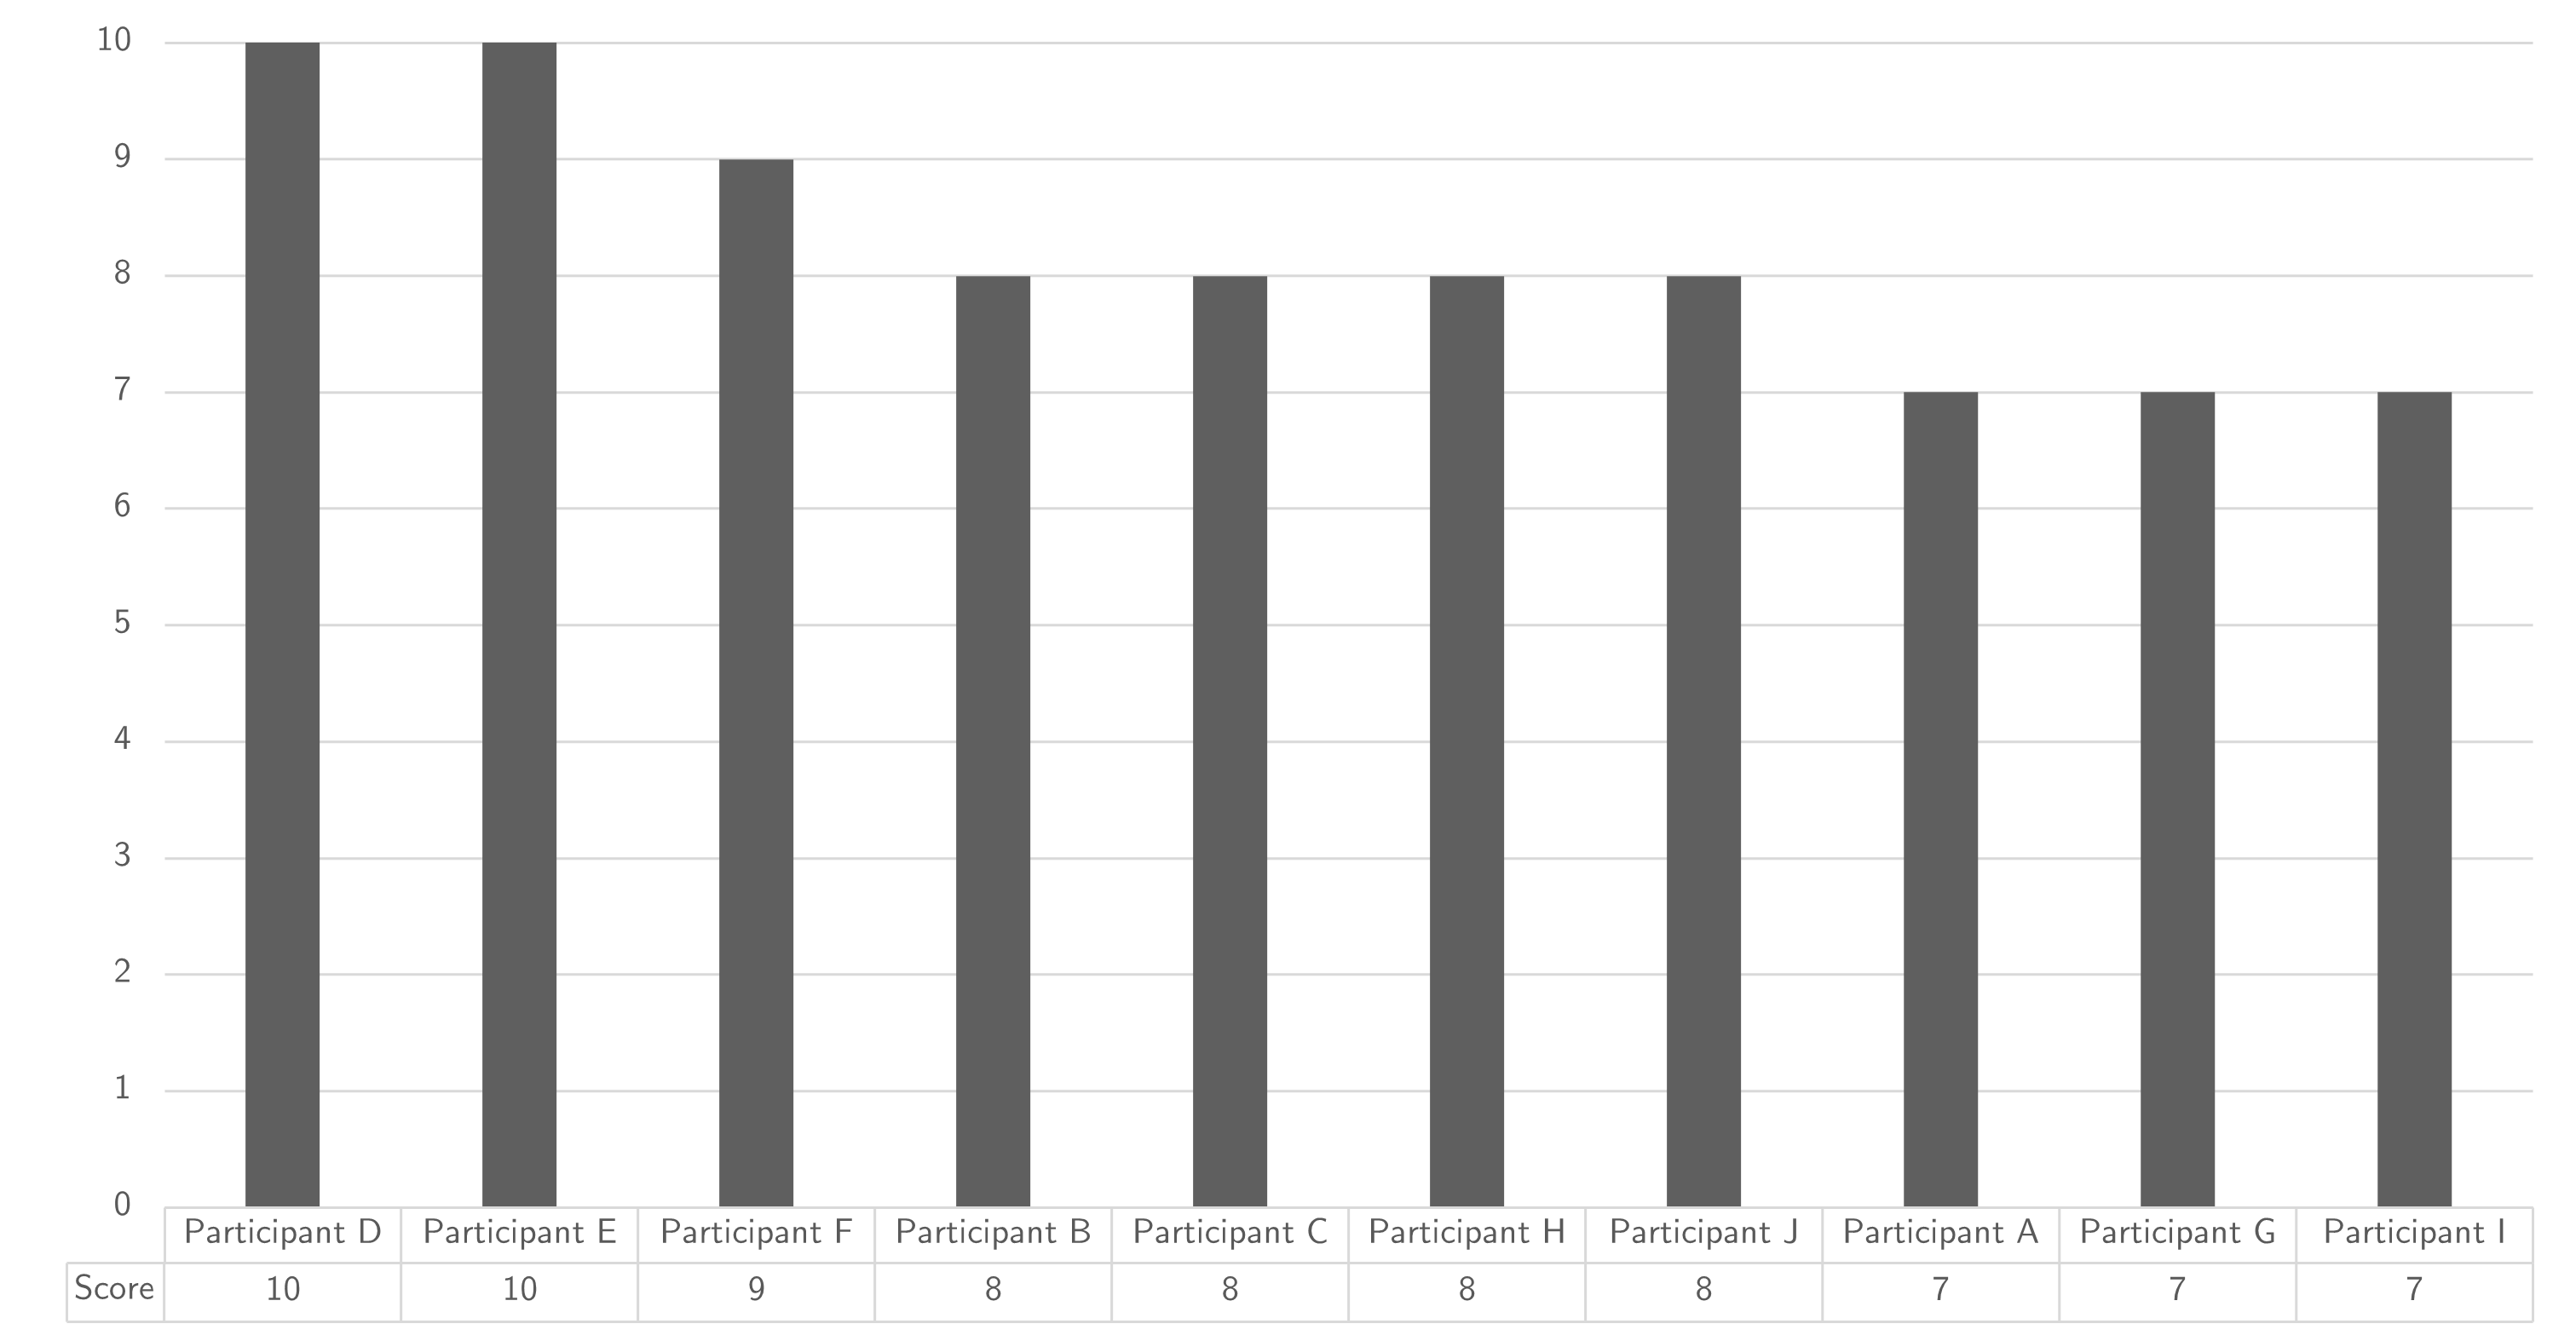
\includegraphics[width=0.9\linewidth]{images/scoreafselforganisation}
	\caption[Scoring of antifragile attribute Self-Organisation]{Scoring of antifragile attribute Self-Organisation}
	\label{fig:appscoringafselforganisation}
\end{figure}
\begin{table}[h!]
	\centering
	\begin{tabular}{p{.55\textwidth}ccc}
		\toprule
		\textbf{Attribute} & \textbf{Rating} & \textbf{Variability} & \textbf{Abstains} \\
		\midrule
		Self-Organisation & 8,2 & 23\% & 0 \\%
		\bottomrule
	\end{tabular}%
	\caption[Scoring of antifragile attribute Self-Organisation]{Scoring of antifragile attribute Self-Organisation}
	\label{tab:appscoringafselforganisation}%
\end{table}%
\newpage
\subsection{Fail-Fast}
\begin{figure}[h!]
	\centering
	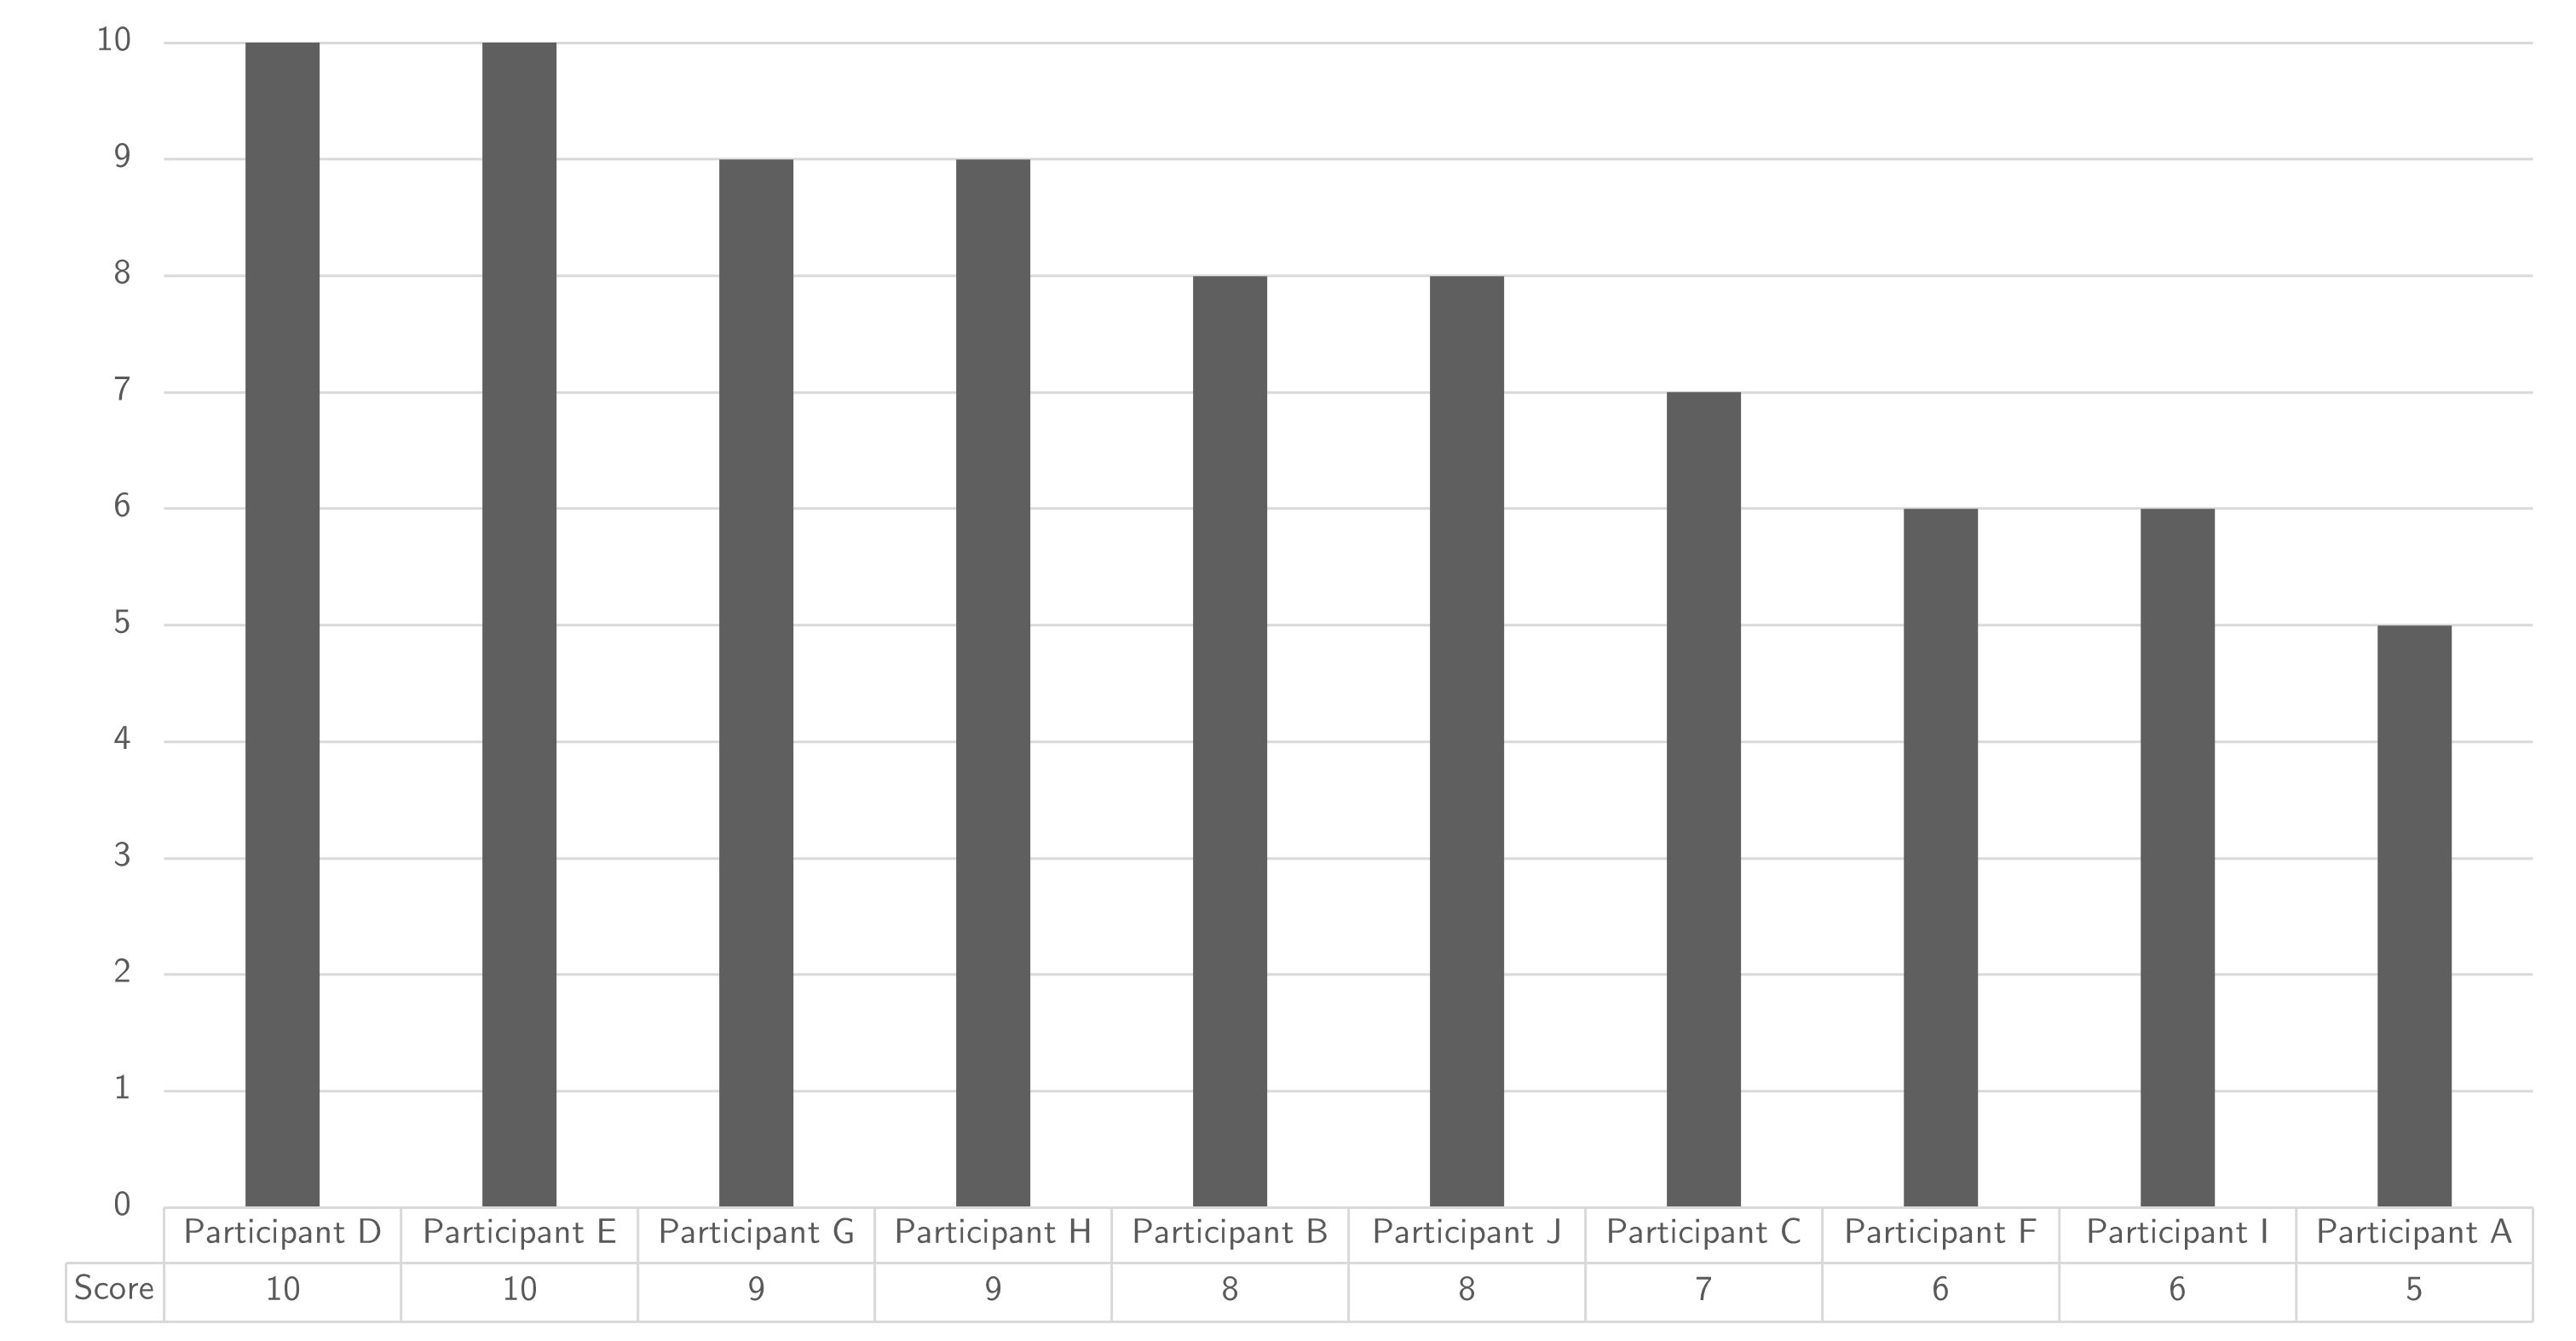
\includegraphics[width=0.9\linewidth]{images/scoreaffailfast}
	\caption[Scoring of antifragile attribute Fail-Fast]{Scoring of antifragile attribute Fail-Fast}
	\label{fig:appscoringaffailfast}
\end{figure}
\begin{table}[h!]
	\centering
	\begin{tabular}{p{.55\textwidth}ccc}
		\toprule
		\textbf{Attribute} & \textbf{Rating} & \textbf{Variability} & \textbf{Abstains} \\
		\midrule
		Fail-Fast & 7,8 & 35\% & 0 \\%
		\bottomrule
	\end{tabular}%
	\caption[Scoring of antifragile attribute Fail-Fast]{Scoring of antifragile attribute Fail-Fast}
	\label{tab:appscoringaffailfast}%
\end{table}%
\newpage
\subsection{Resources to invest}
\begin{figure}[h!]
	\centering
	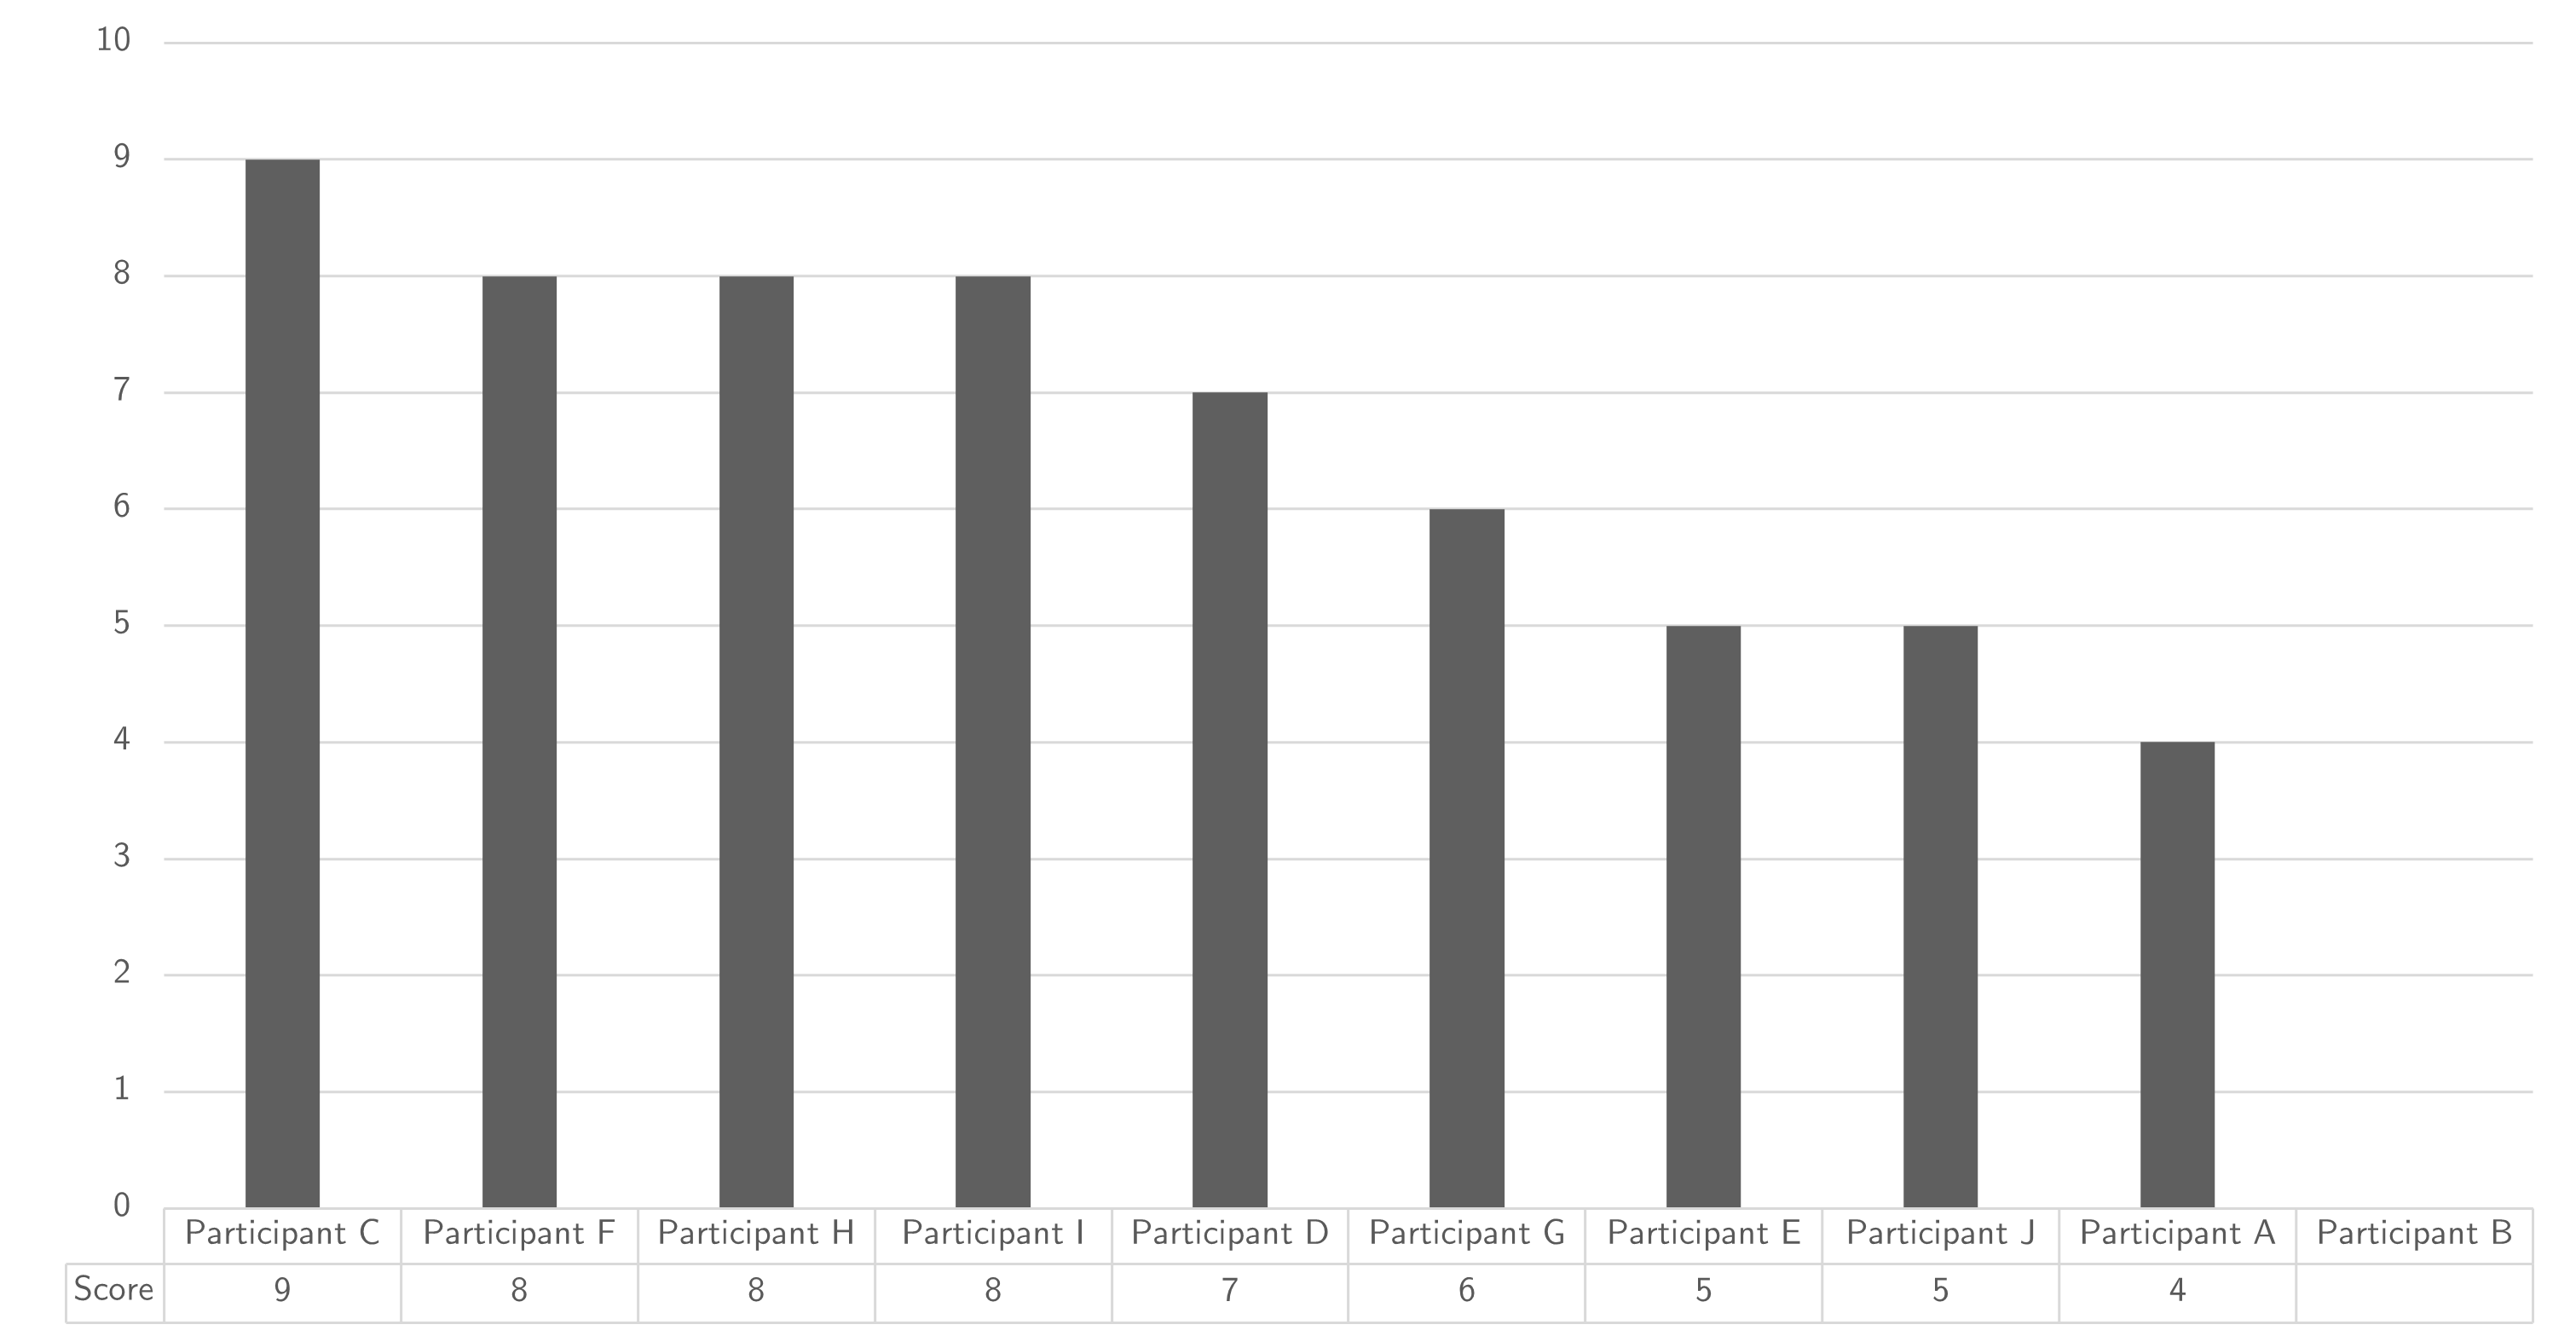
\includegraphics[width=0.9\linewidth]{images/scoreafresourcestoinvest}
	\caption[Scoring of antifragile attribute Resources to Invest]{Scoring of antifragile attribute Resources to Invest}
	\label{fig:appscoringafresourcestoinvest}
\end{figure}
\begin{table}[h!]
	\centering
	\begin{tabular}{p{.55\textwidth}ccc}
		\toprule
		\textbf{Attribute} & \textbf{Rating} & \textbf{Variability} & \textbf{Abstains} \\
		\midrule
		Resources to Invest & 6,7 & 36\% & 1 \\%
		\bottomrule
	\end{tabular}%
	\caption[Scoring of antifragile attribute Resources to Invest]{Scoring of antifragile attribute Resources to Invest}
	\label{tab:appscoringafresourcestoinvest}%
\end{table}%
\newpage
\subsection{Senenca's Barbell}
\begin{figure}[h!]
	\centering
	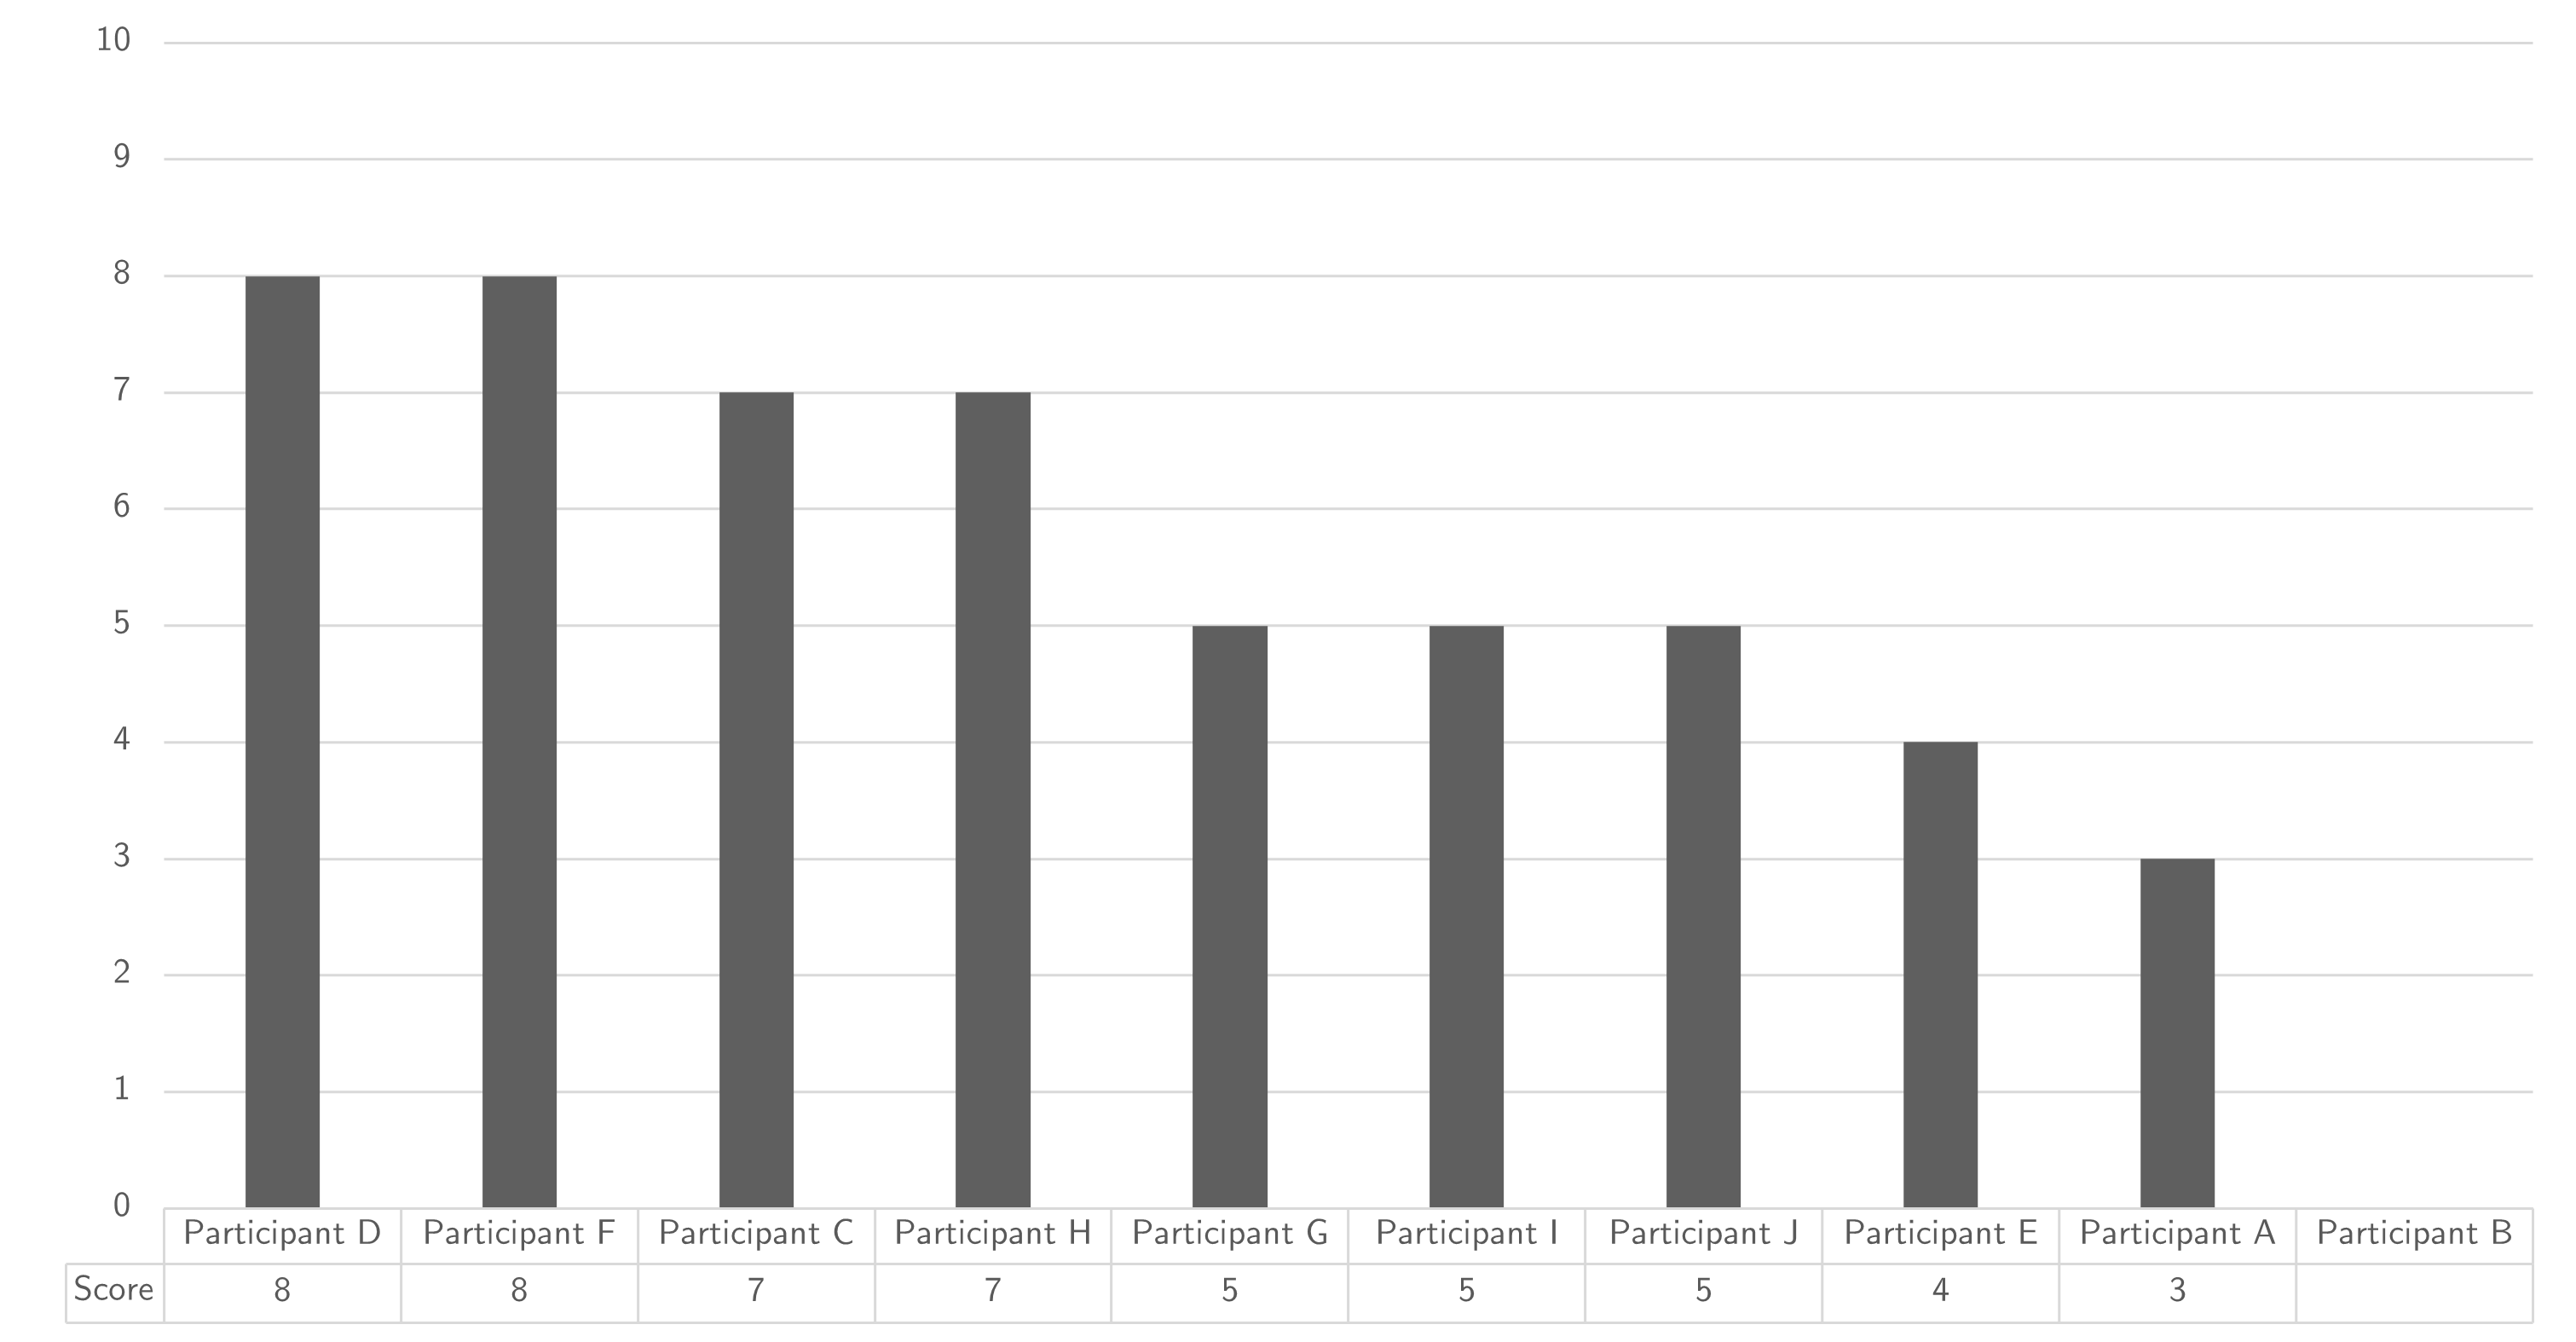
\includegraphics[width=0.9\linewidth]{images/scoreafseneca}
	\caption[Scoring of antifragile attribute Seneca's Barbell]{Scoring of antifragile attribute Seneca's Barbell}
	\label{fig:appscoringafseneca}
\end{figure}
\begin{table}[h!]
	\centering
	\begin{tabular}{p{.55\textwidth}ccc}
		\toprule
		\textbf{Attribute} & \textbf{Rating} & \textbf{Variability} & \textbf{Abstains} \\
		\midrule
		Seneca's Barbell & 5,8 & 37\% & 1 \\%
		\bottomrule
	\end{tabular}%
	\caption[Scoring of antifragile attribute Seneca's Barbell]{Scoring of antifragile attribute Seneca's Barbell}
	\label{tab:appscoringafseneca}%
\end{table}%
\newpage
\subsection{Safe working environment}
\begin{figure}[h!]
	\centering
	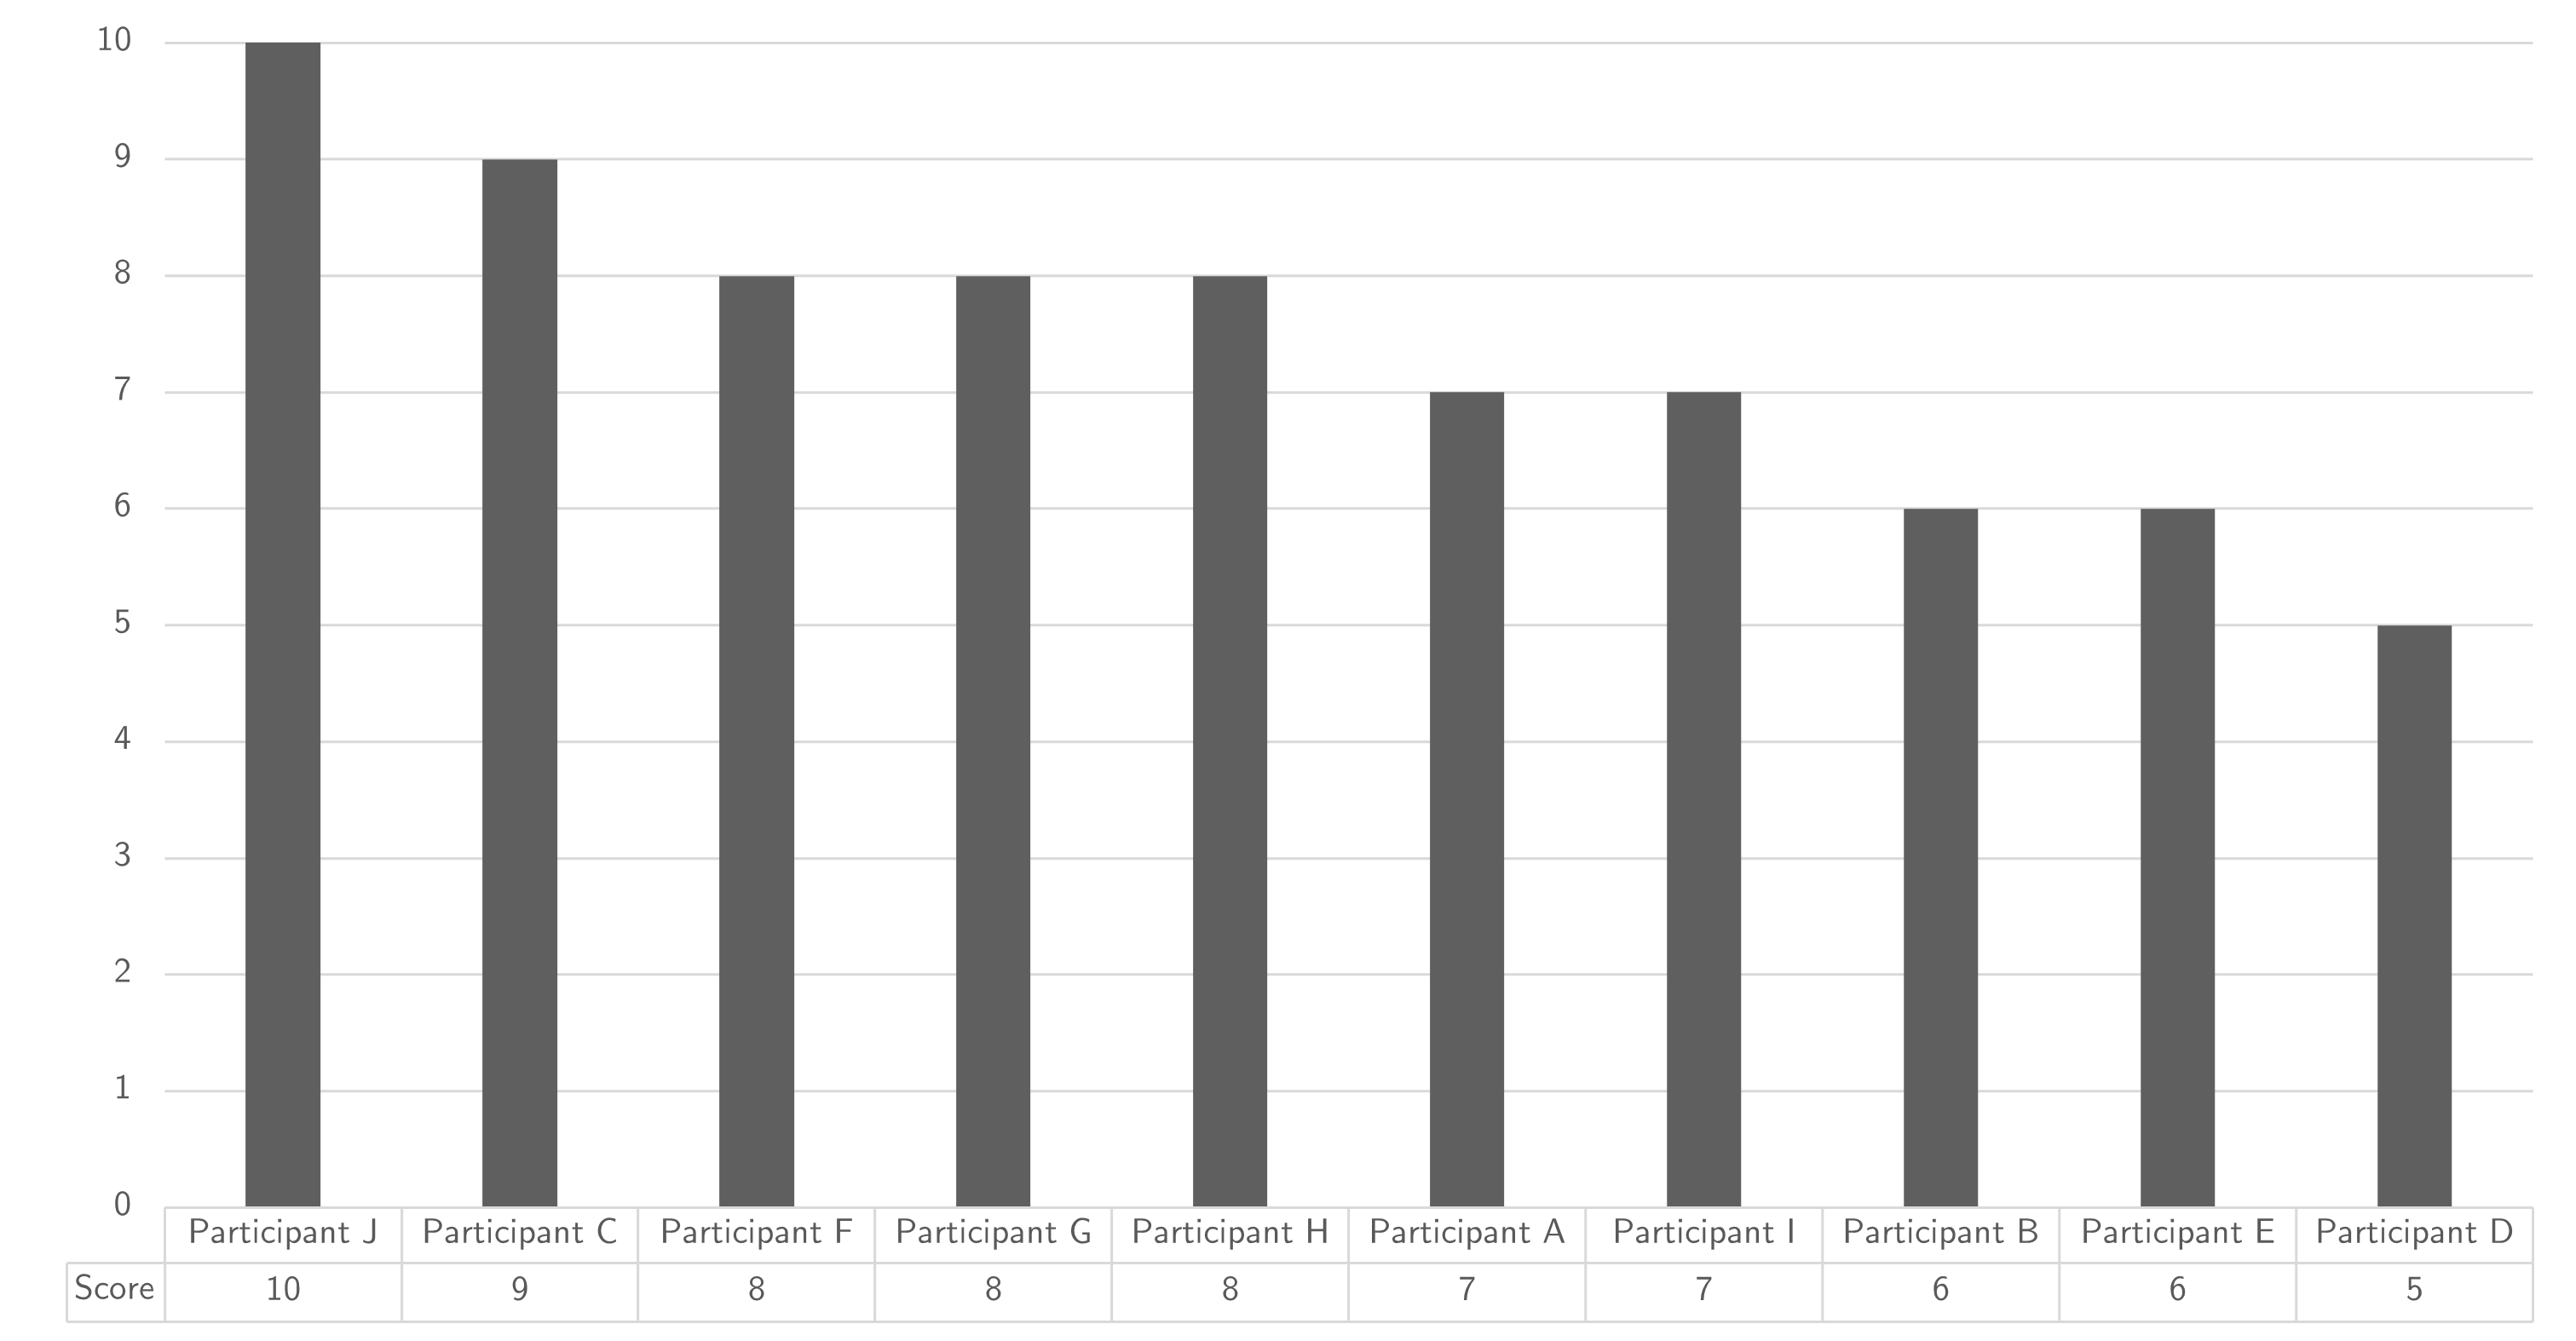
\includegraphics[width=0.9\linewidth]{images/scoreafsafeworkingenvironnment}
	\caption[Scoring of antifragile attribute Safe working environment]{Scoring of antifragile attribute Safe working environment}
	\label{fig:appscoringafsafeworkingenvironnment}
\end{figure}
\begin{table}[h!]
	\centering
	\begin{tabular}{p{.55\textwidth}ccc}
		\toprule
		\textbf{Attribute} & \textbf{Rating} & \textbf{Variability} & \textbf{Abstains} \\
		\midrule
		Safe working environment & 7,4 & 31\% & 0 \\%
		\bottomrule
	\end{tabular}%
	\caption[Scoring of antifragile attribute Safe working environment]{Scoring of antifragile attribute Safe working environment}
	\label{tab:appscoringafsafeworkingenvironment}%
\end{table}%
\newpage
\subsection{Naar buiten kijken, samenwerking zoeken}
\begin{figure}[h!]
	\centering
	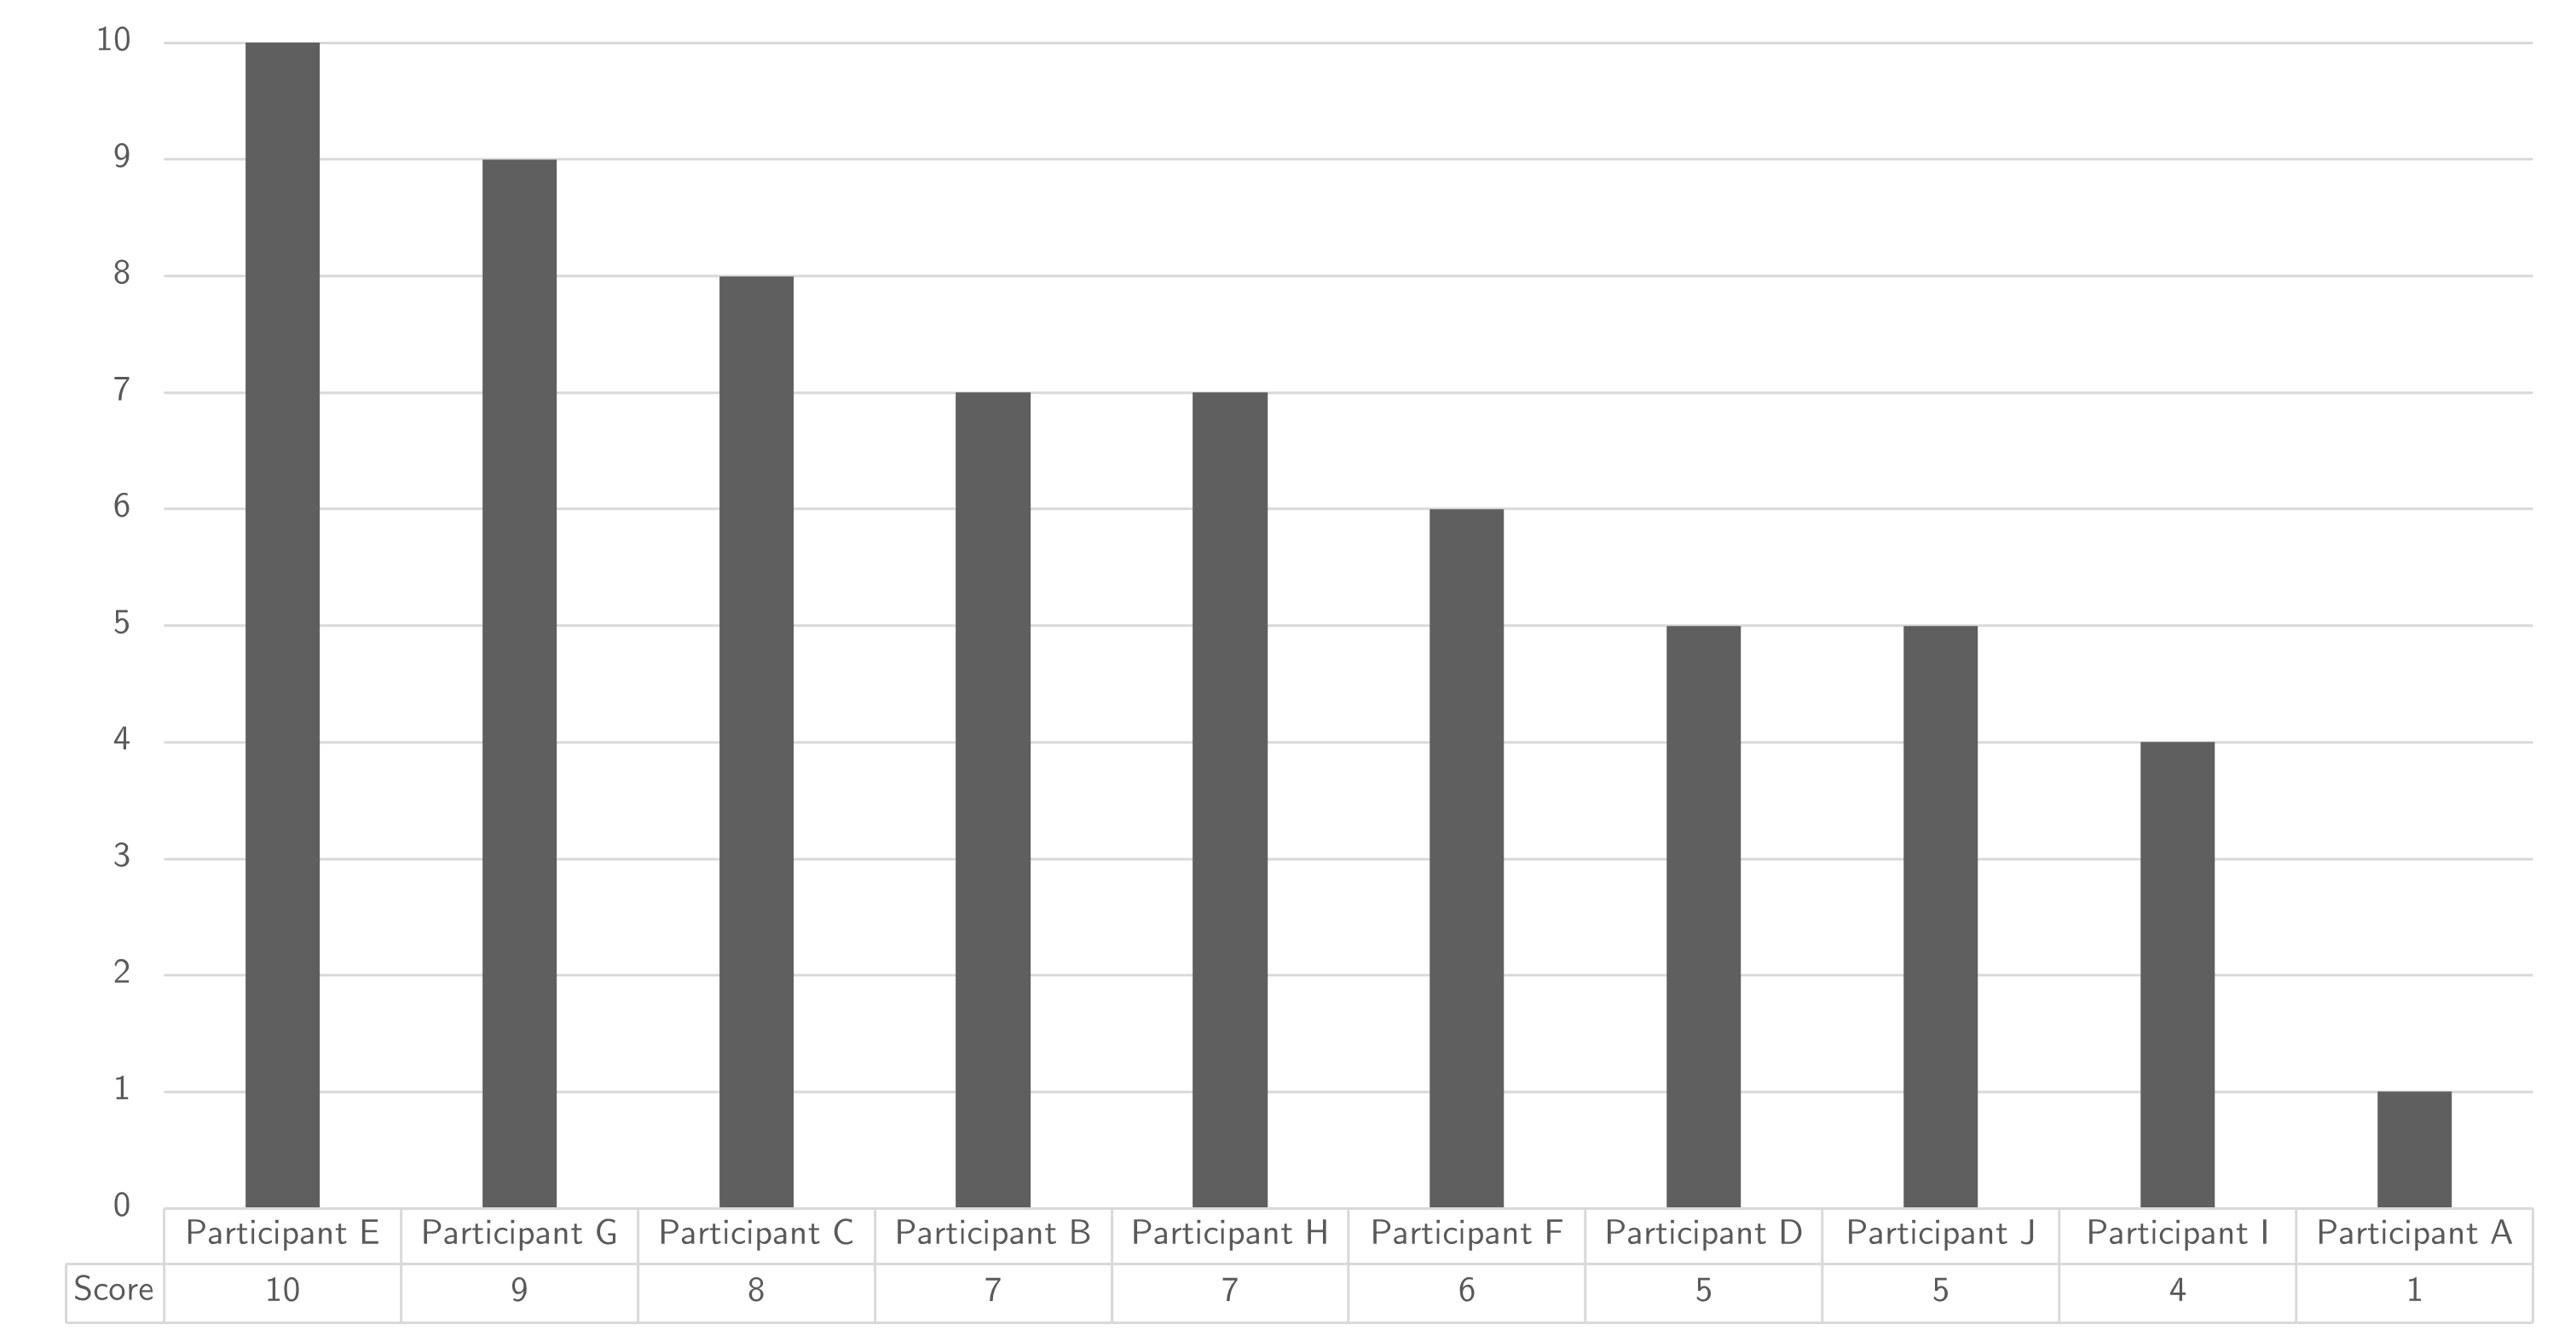
\includegraphics[width=0.9\linewidth]{images/scoreafnaarbuitenkijken}
	\caption[Scoring of antifragile attribute Naar buiten kijken]{Scoring of antifragile attribute Naar buiten kijken}
	\label{fig:appscoringafnaarbuiten}
\end{figure}
\begin{table}[h!]
	\centering
	\begin{tabular}{p{.55\textwidth}ccc}
		\toprule
		\textbf{Attribute} & \textbf{Rating} & \textbf{Variability} & \textbf{Abstains} \\
		\midrule
		Naar buiten kijken, samenwerking zoeken & 6,2 & 55\% & 0 \\%
		\bottomrule
	\end{tabular}%
	\caption[Scoring of antifragile attribute Naar buiten]{Scoring of antifragile attribute Naar buiten}
	\label{tab:appscoringafnaarbuitenkijken}%
\end{table}%
\newpage
\subsection{Data Governance Planes}
\begin{figure}[h!]
	\centering
	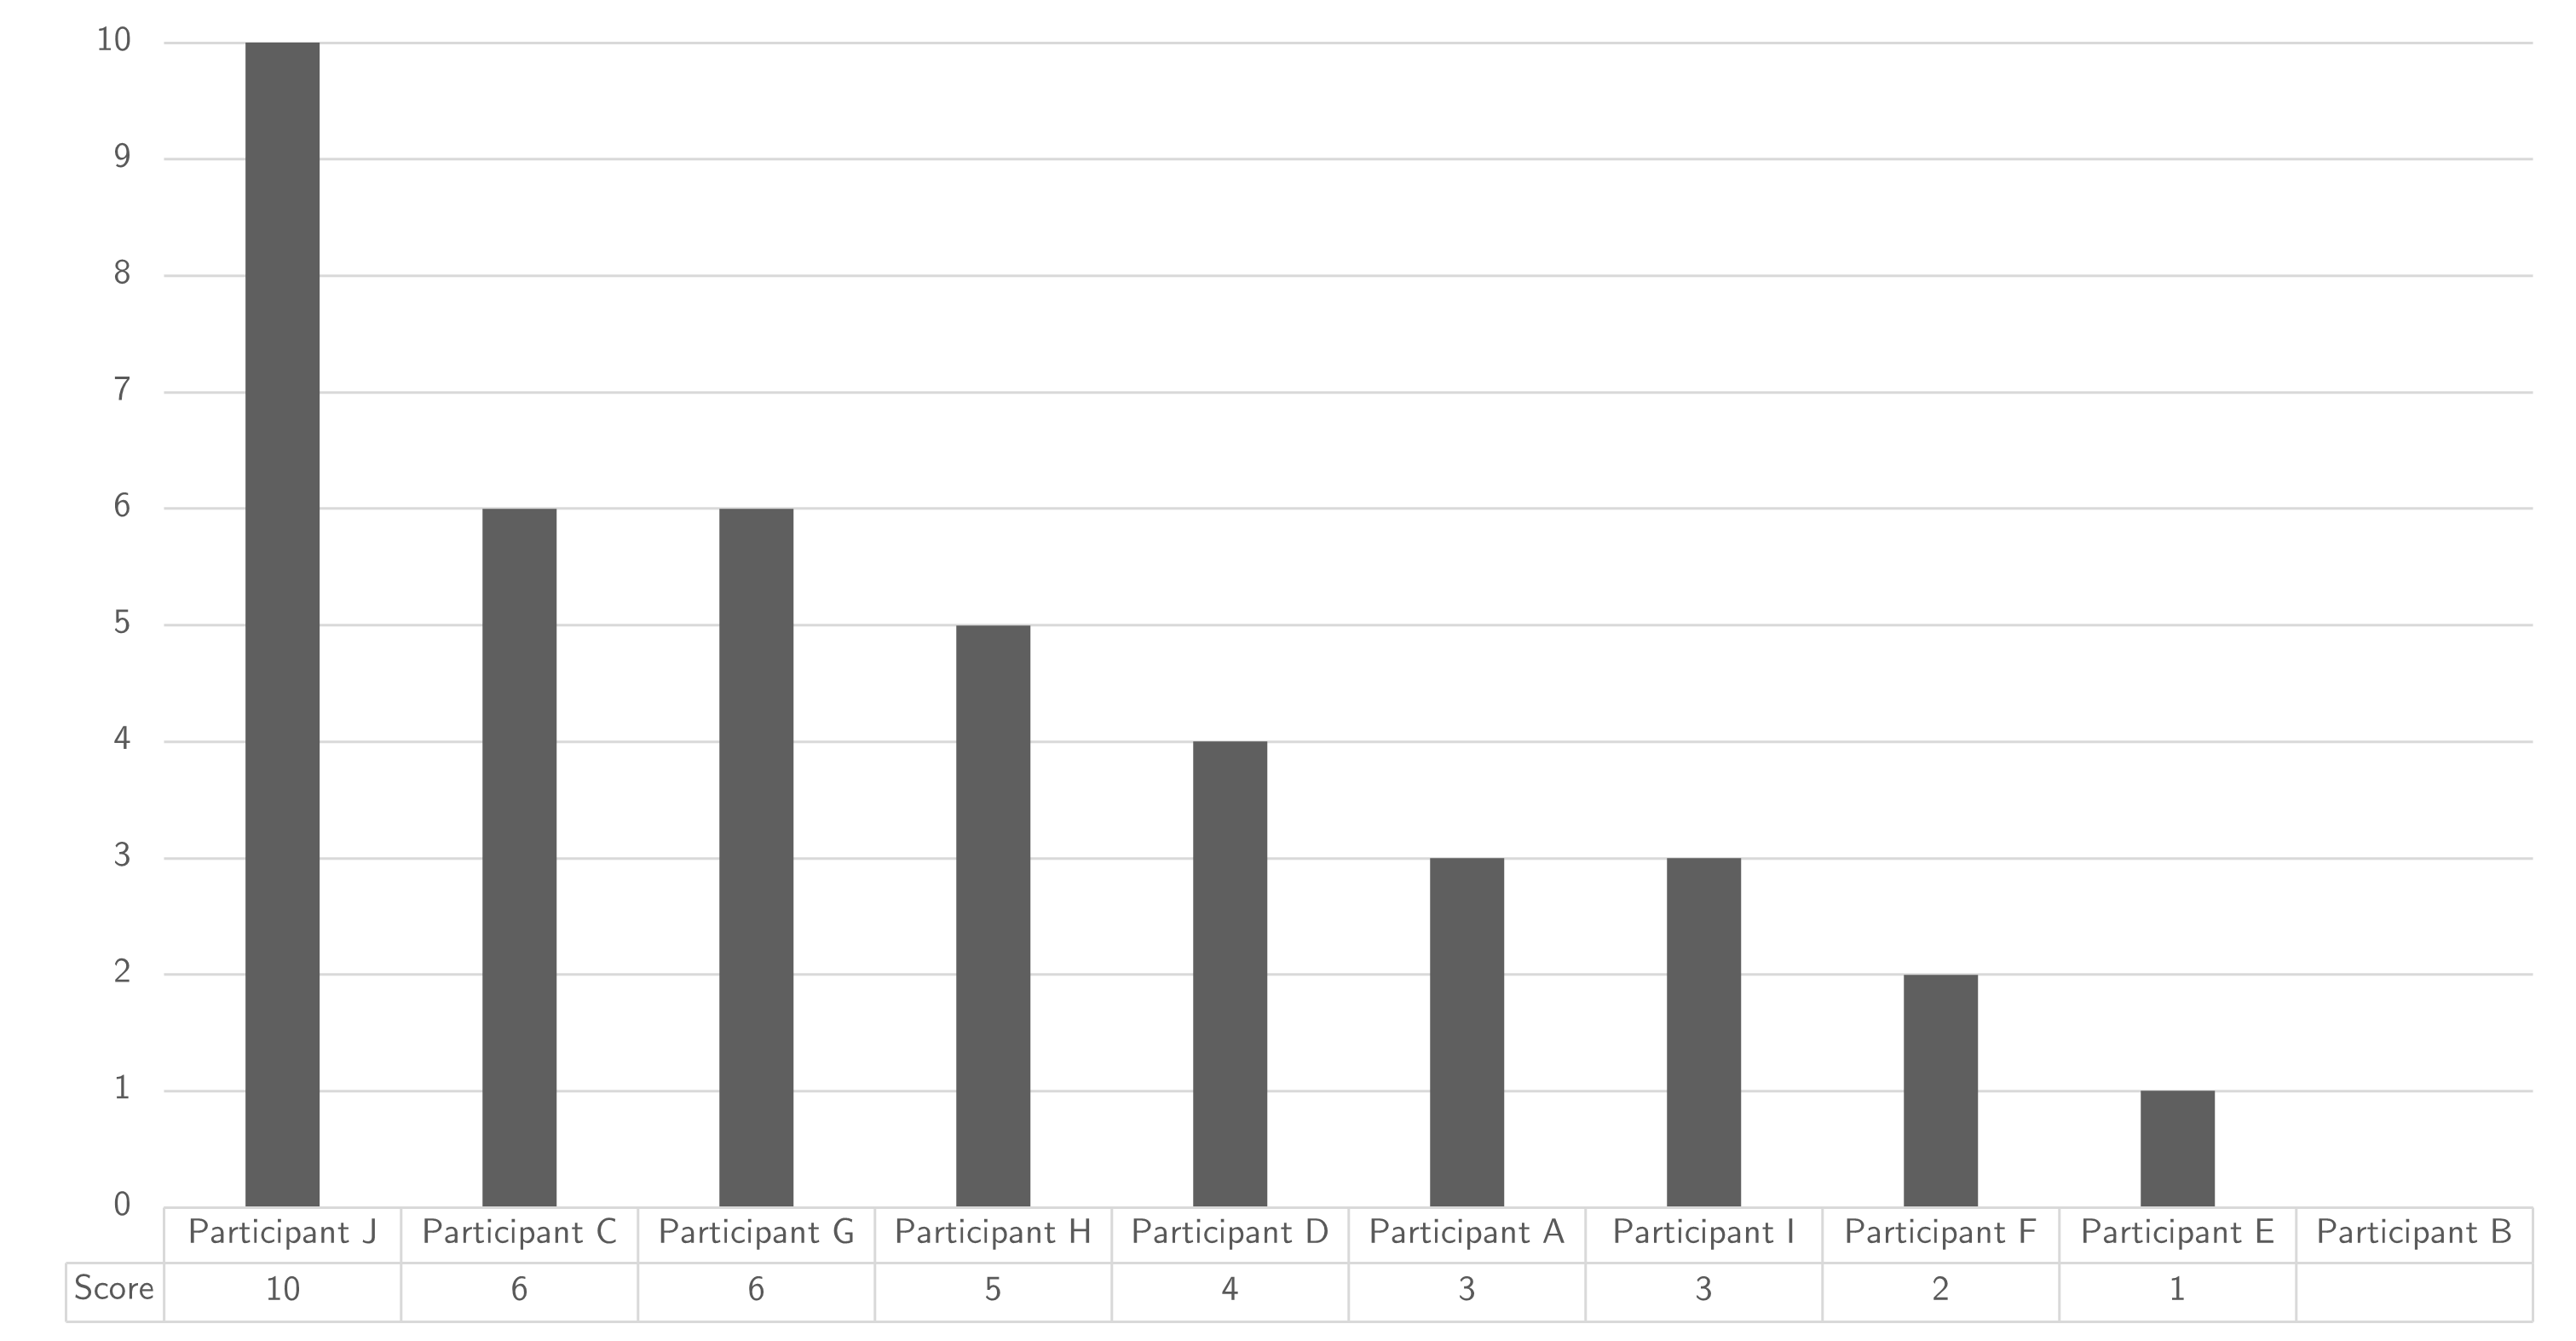
\includegraphics[width=0.9\linewidth]{images/scoreafdatagovernanceplanes}
	\caption[Scoring of antifragile attribute Data Governance Planes]{Scoring of antifragile attribute Data Governance Planes}
	\label{fig:appscoringafdatagovernanceplanes}
\end{figure}
\begin{table}[h!]
	\centering
	\begin{tabular}{ccc}
		\toprule
		\textbf{Rating} & \textbf{Variability} & \textbf{Abstains} \\
		\midrule
		4,4 & 56\% & 1 \\%
		\bottomrule
	\end{tabular}%
	\caption[Scoring of antifragile attribute Data Governance Planes]{Scoring of antifragile attribute Data Governance Planes}
	\label{tab:appscoringafdatagovernance}
\end{table}%
\newpage
\section{Validation of Enterprise Architecture schools of thought}
\begin{table}[!h]
	\centering
	\begin{tabular}{p{.55\textwidth}ccc}
		\toprule
		\textbf{School} & \textbf{Rating} & \textbf{Variability} & \textbf{Abstains} \\
		\midrule
		Enterprise IT Architecting & 5,6 & 34\% & 0 \\%
		Enterprise Integrating & 7,2 & 16\% & 0 \\%
		Enterprise Ecological Adaptation & 8,8 & 27\% & 0 \\%
		\bottomrule
	\end{tabular}%
	\caption{Validation of Enterprise Architecture schools of thought}
	\label{tab:appvalidationofeaschools}%
\end{table}%
\subsection{Enterprise IT Architecting}
\begin{figure}[h!]
	\centering
	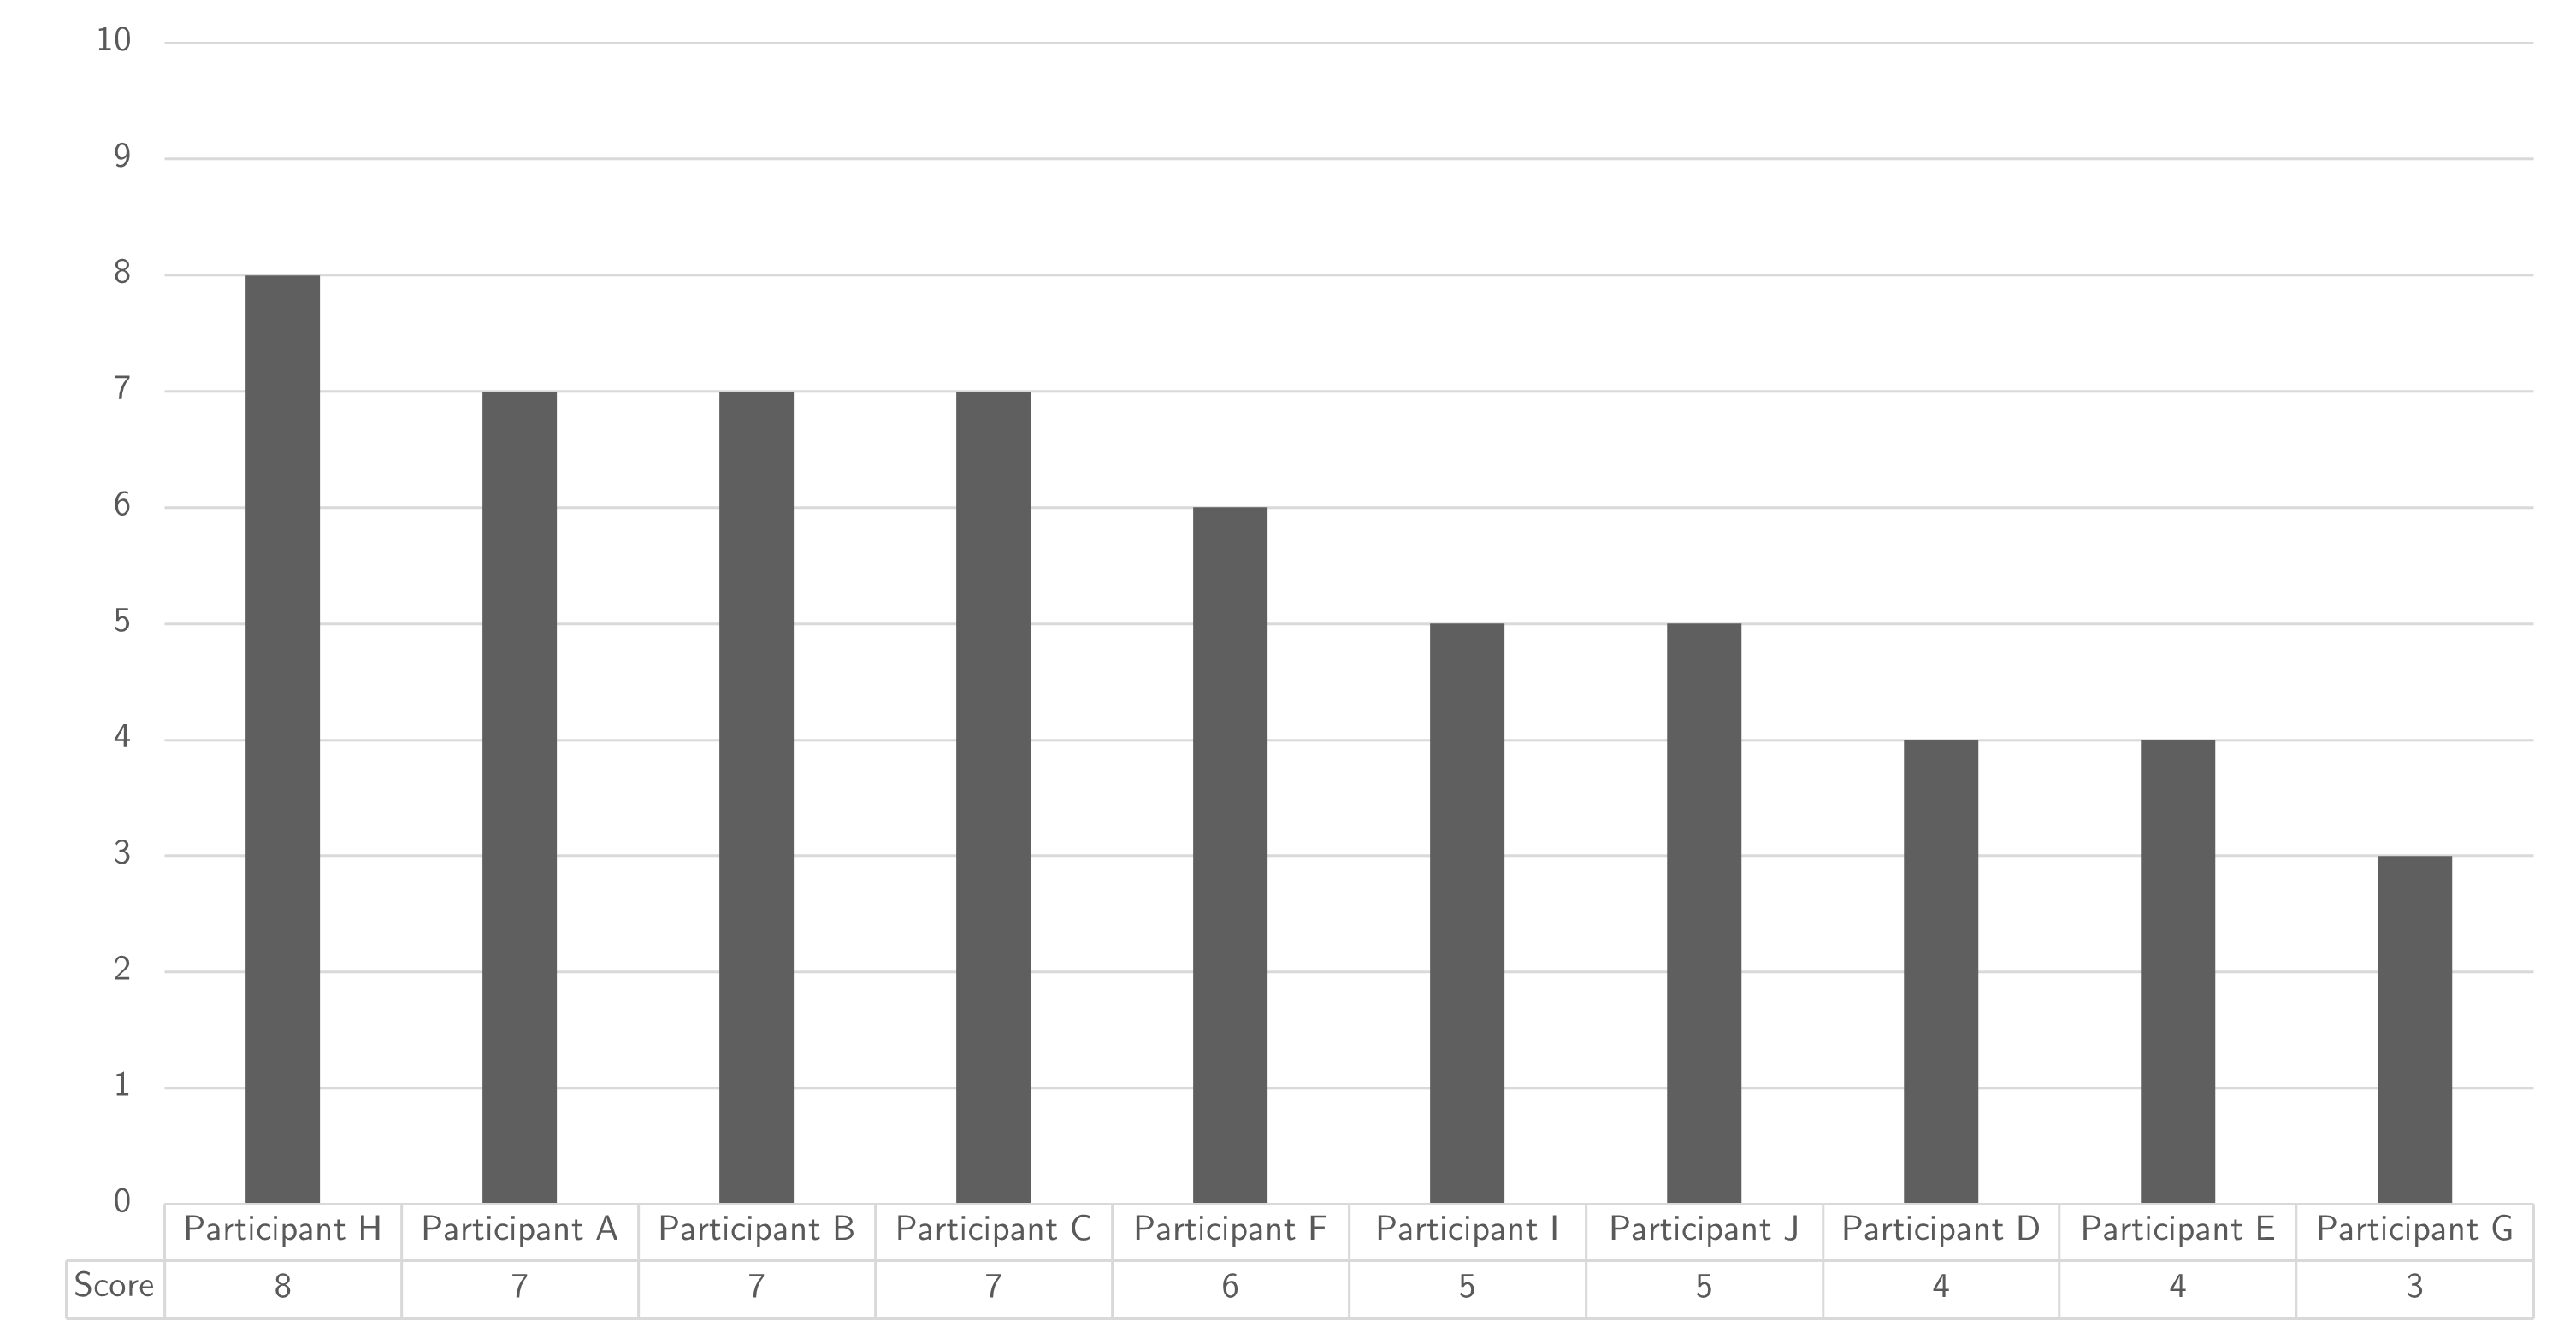
\includegraphics[width=0.9\linewidth]{images/scoreeaschoolenterpriseitarchitecting}
	\caption[Scoring of school of thought Enterprise IT Architecting]{Scoring of school of thought Enterprise IT Architecting}
	\label{fig:appscoringschoolenterpriseitarchitecting}
\end{figure}
\begin{table}[h!]
	\centering
	\begin{tabular}{p{.55\textwidth}ccc}
		\toprule
		\textbf{Attribute} & \textbf{Rating} & \textbf{Variability} & \textbf{Abstains} \\
		\midrule
		Enterprise IT Architecting & 5,6 & 34\% & 0 \\%
		\bottomrule
	\end{tabular}%
	\caption[Scoring of school of thought Enterprise IT Architecting]{Scoring of school of thought Enterprise IT Architecting}
	\label{tab:appscoringschoolenterpriseitarchitecting}%
\end{table}%

\newpage
\subsection{Enterprise Integrating}
\begin{figure}[h!]
	\centering
	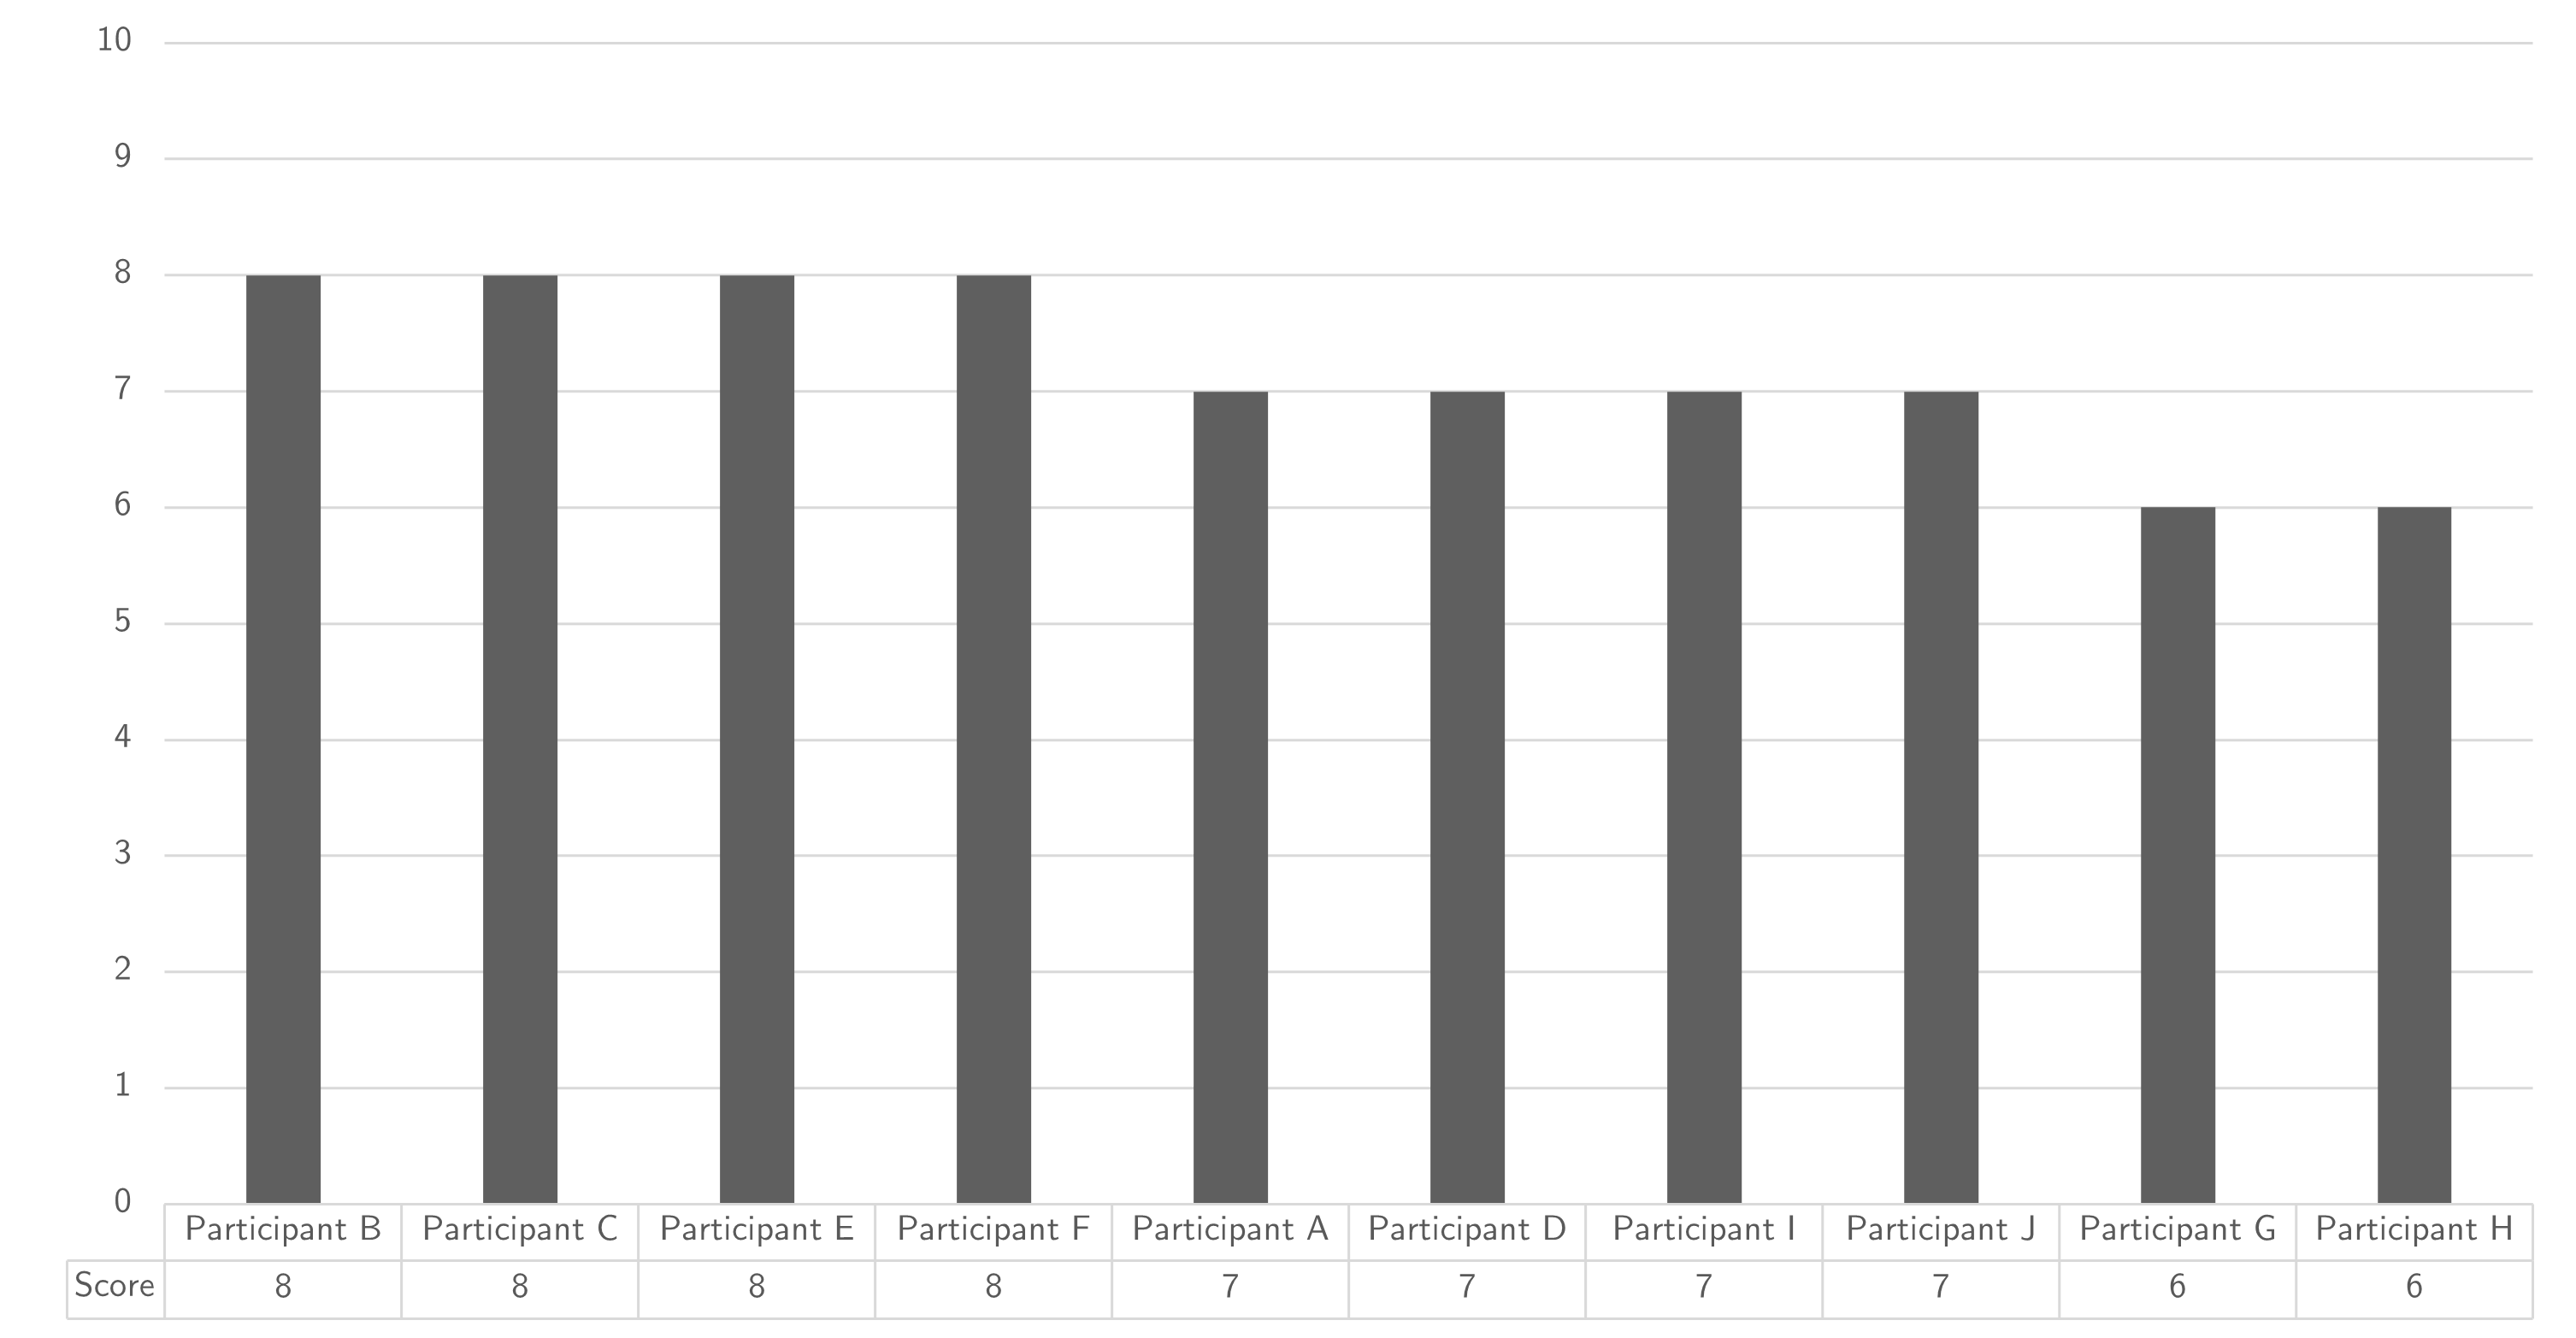
\includegraphics[width=0.9\linewidth]{images/scoreeaschoolenterpriseintegrating}
	\caption[Scoring of school of thought Enterprise Integrating]{Scoring of school of thought Enterprise Integrating}
	\label{fig:appscoringschoolenterpriseintegrating}
\end{figure}
\begin{table}[h!]
	\centering
	\begin{tabular}{p{.55\textwidth}ccc}
		\toprule
		\textbf{Attribute} & \textbf{Rating} & \textbf{Variability} & \textbf{Abstains} \\
		\midrule
		Enterprise Integrating & 7,2 & 16\% & 0 \\%
		\bottomrule
	\end{tabular}%
	\caption[Scoring of school of thought Enterprise Integrating]{Scoring of school of thought Enterprise Integrating}
	\label{tab:appscoringschoolenterpriseintegrating}%
\end{table}%
\newpage
\subsection{Enterprise Ecological Adaptation}
\begin{figure}[h!]
	\centering
	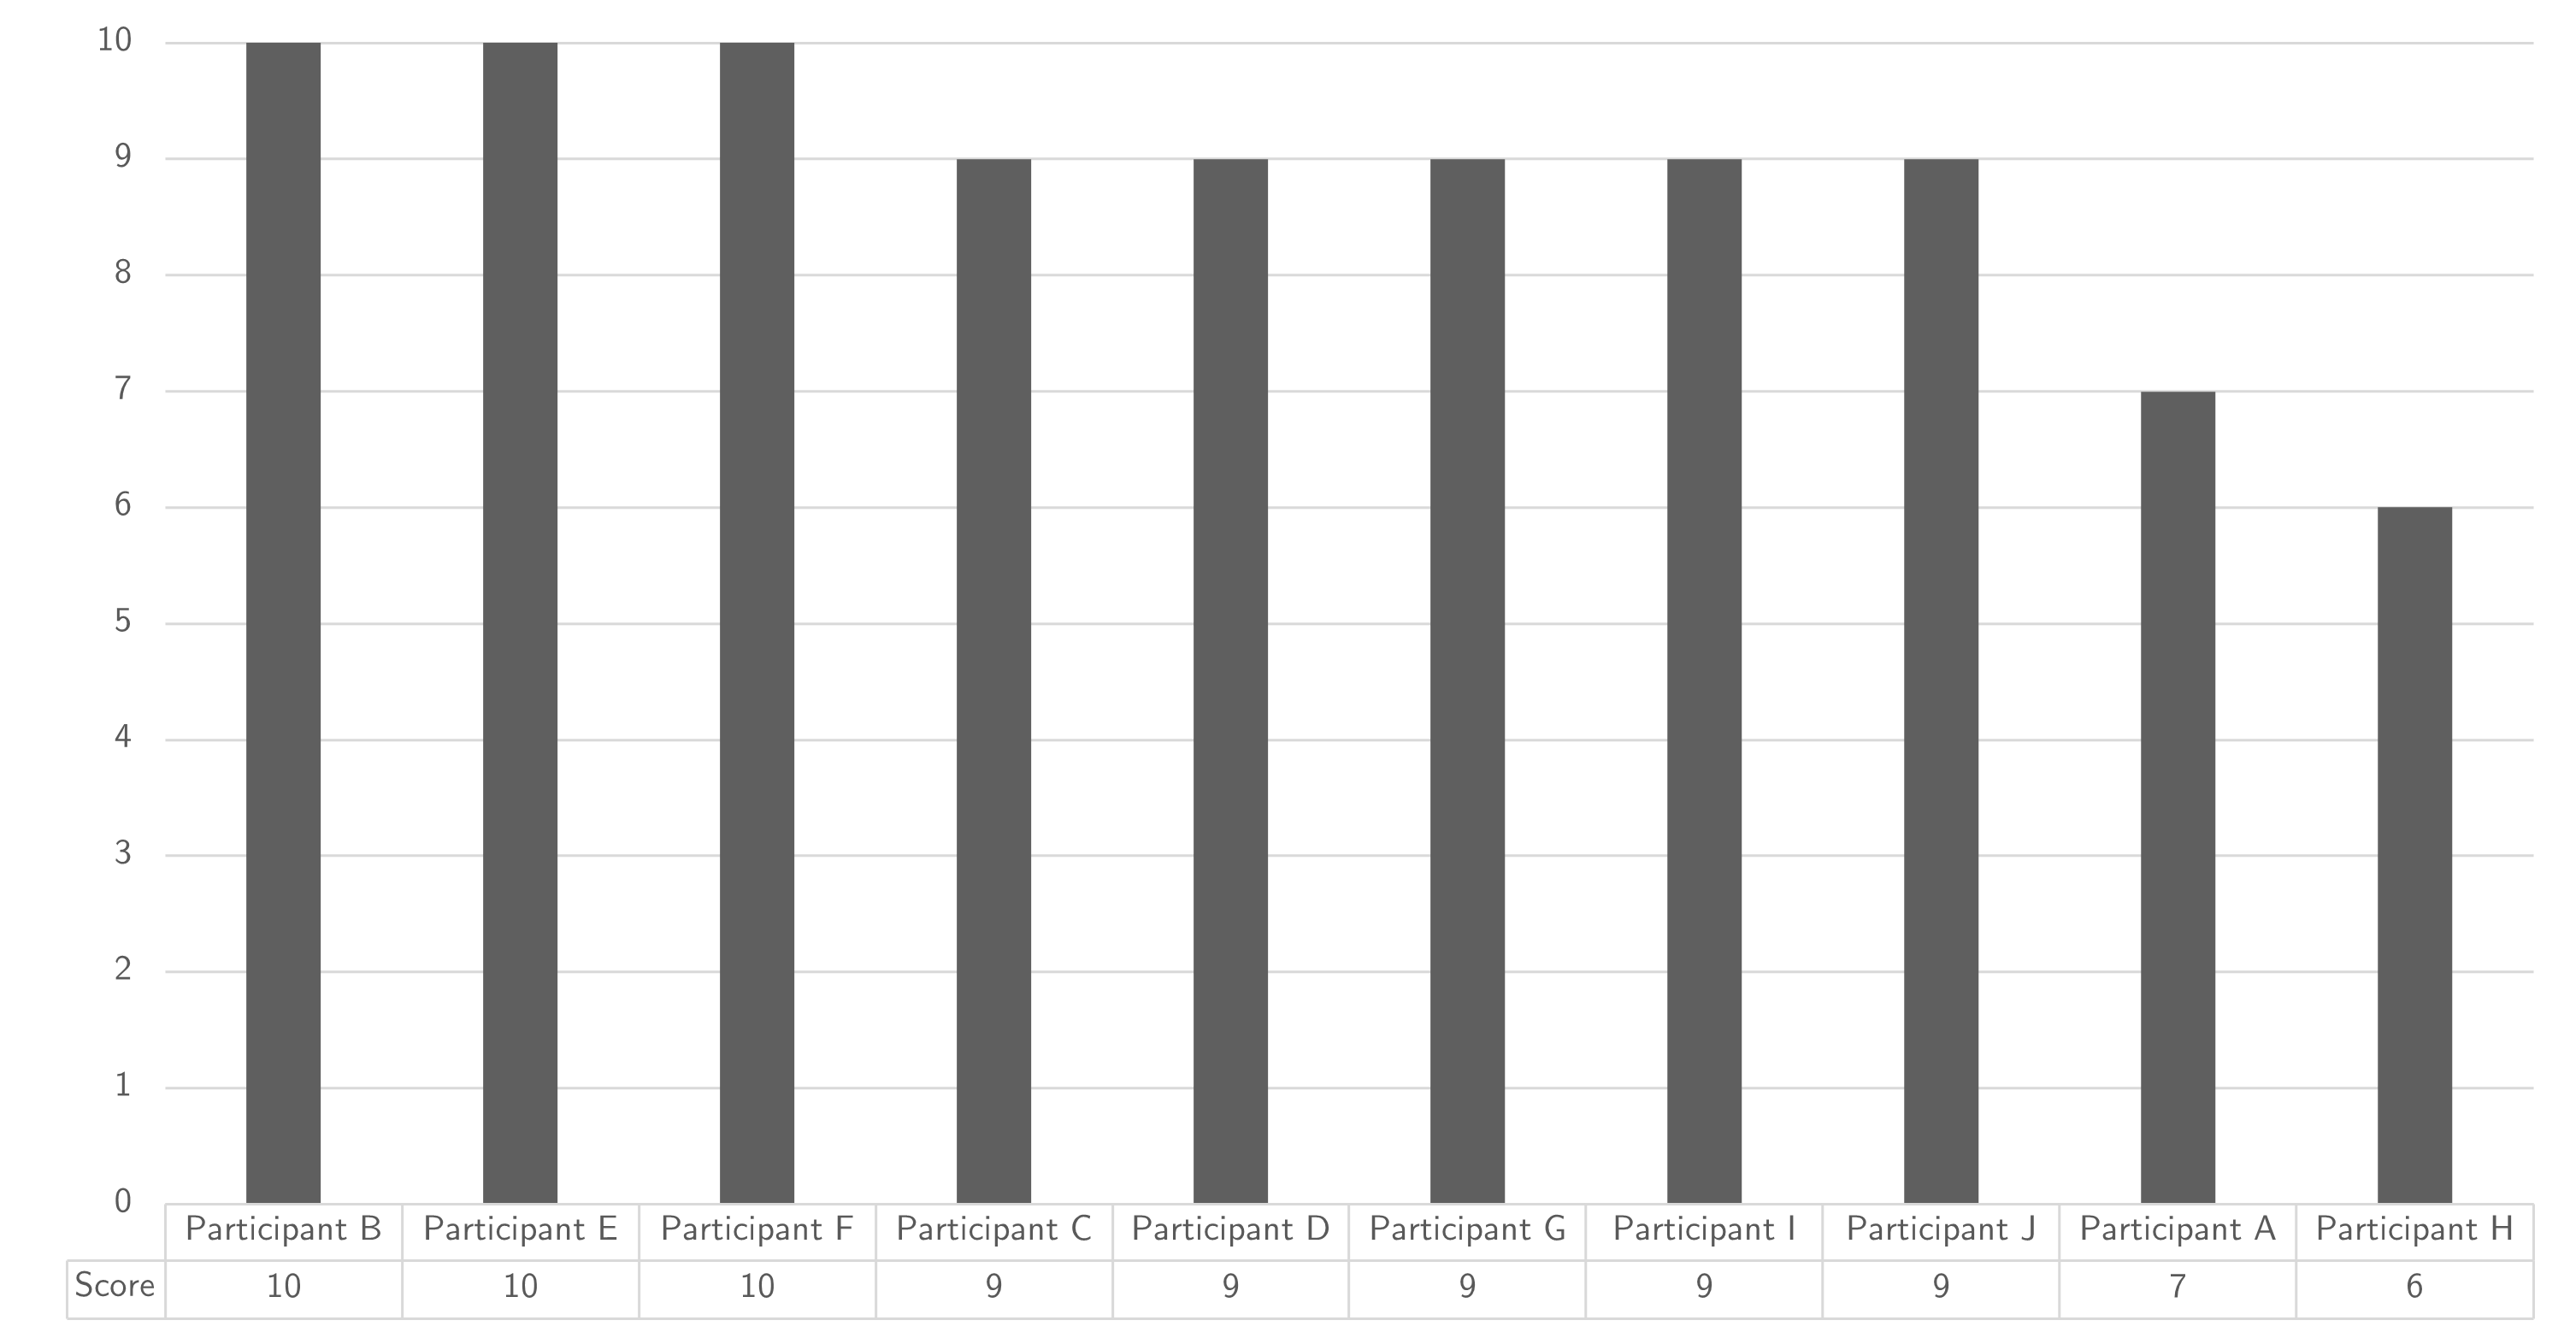
\includegraphics[width=0.9\linewidth]{images/scoreeaschoolenterpriseecologicaladaptation}
	\caption[Scoring of school of thought Enterprise Ecological Adaptation]{Scoring of school of thought Enterprise Ecological Adaptation}
	\label{fig:appscoringschoolenterpriseecologicaladaptation}
\end{figure}
\begin{table}[h!]
	\centering
	\begin{tabular}{p{.55\textwidth}ccc}
		\toprule
		\textbf{Attribute} & \textbf{Rating} & \textbf{Variability} & \textbf{Abstains} \\
		\midrule
		Enterprise Ecological Adaptation & 8,8 & 27\% & 0 \\%
		\bottomrule
	\end{tabular}%
	\caption[Scoring of school of thought Enterprise Ecological Adaptation]{Scoring of school of thought Enterprise Ecological Adaptation}
	\label{tab:appscoringschoolenterpriseecologicaladaptation}%
\end{table}%

\newpage
\section{Validation of Enterprise Architecture attributes}
\begin{table}[!h]
	\centering
	\begin{tabular}{p{.55\textwidth}ccc}
		\toprule
		\textbf{Attribute} & \textbf{Rating} & \textbf{Variability} & \textbf{Abstains} \\
		\midrule
		Systems-in-environment thinking & 7,7 & 28\% & 0 \\%
		Holist (systemic) stance & 7 & 47\% & 0 \\%
		Organisational learning & 7,3 & 44\% & 0 \\%
		Environmental learning & 7,7 & 29\% & 0 \\%
		Intra-organisational coherency & 6,4 & 31\% & 0 \\%
		System-in-environment coevolution learning & 6,6 & 36\% & 0 \\%
		Adapt to business language & 7,1 & 35\% & 0 \\%
		Agile Enterprise & 6,4 & 50\% & 0 \\%
		Real Time Trust (Policy \& Attribute based) & 5,6 & 54\% & 1 \\%
		Foster Dialogue & 6,9 & 32\% & 0 \\%
		Validation & 7,4 & 24\% & 0 \\%
		Altijd goed architectuur & 5,8 & 46\% & 1 \\%
		\bottomrule
	\end{tabular}%
	\caption{Validation of Enterprise Architecture attributes}
	\label{tab:appvalidationofeaattributes}%
\end{table}%
\newpage
\subsection{Systems-in-Environment thinking}
\begin{figure}[h!]
	\centering
	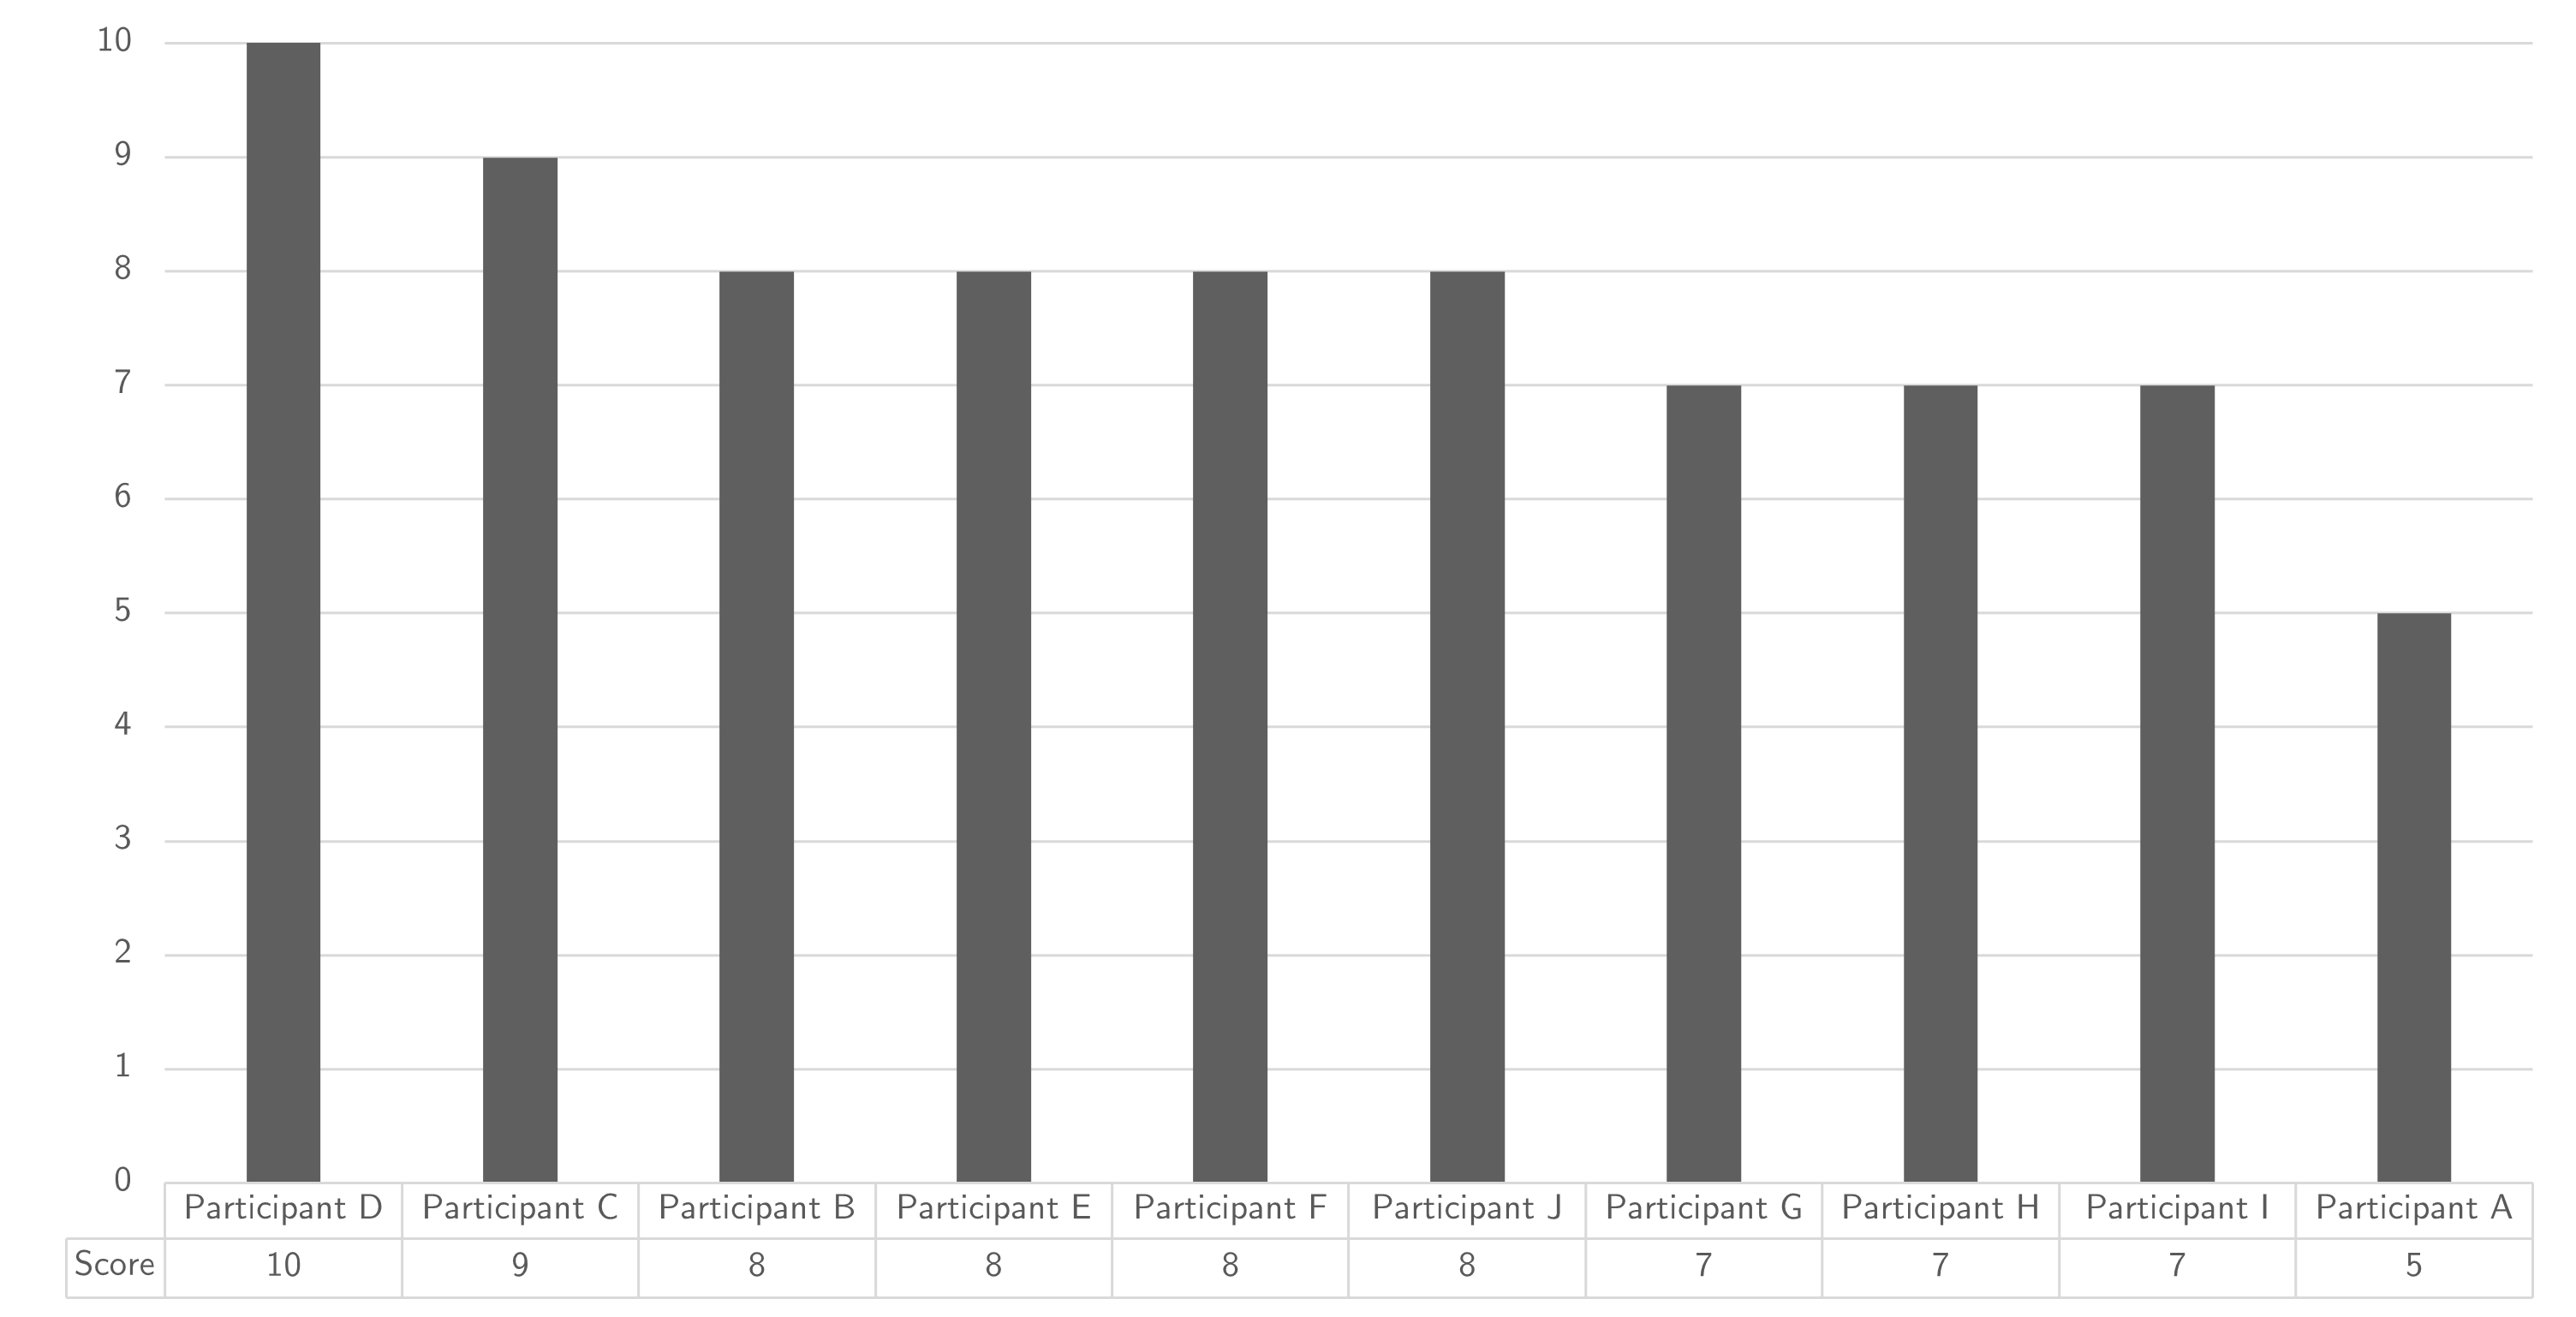
\includegraphics[width=0.9\linewidth]{images/scoreeasystemsinenvironmentthinking}
	\caption[Scoring of EA attribute Systems-in-Environment thinking]{Scoring of EA attribute Systems-in-Environment thinking}
	\label{fig:appscoringeasystemsinenvironmentthinking}
\end{figure}
\begin{table}[h!]
	\centering
	\begin{tabular}{p{.55\textwidth}ccc}
		\toprule
		\textbf{Attribute} & \textbf{Rating} & \textbf{Variability} & \textbf{Abstains} \\
		\midrule
		Systems-in-environment thinking & 7,7 & 28\% & 0 \\%
		\bottomrule
	\end{tabular}%
	\caption[Scoring of EA attribute Systems-in-Environment thinking]{Scoring of EA attribute Systems-in-Environment thinking}
	\label{tab:appscoringeasystemsinenvironmentthinking}%
\end{table}%
\newpage
\subsection{Holistic (systemic) stance}
\begin{figure}[h!]
	\centering
	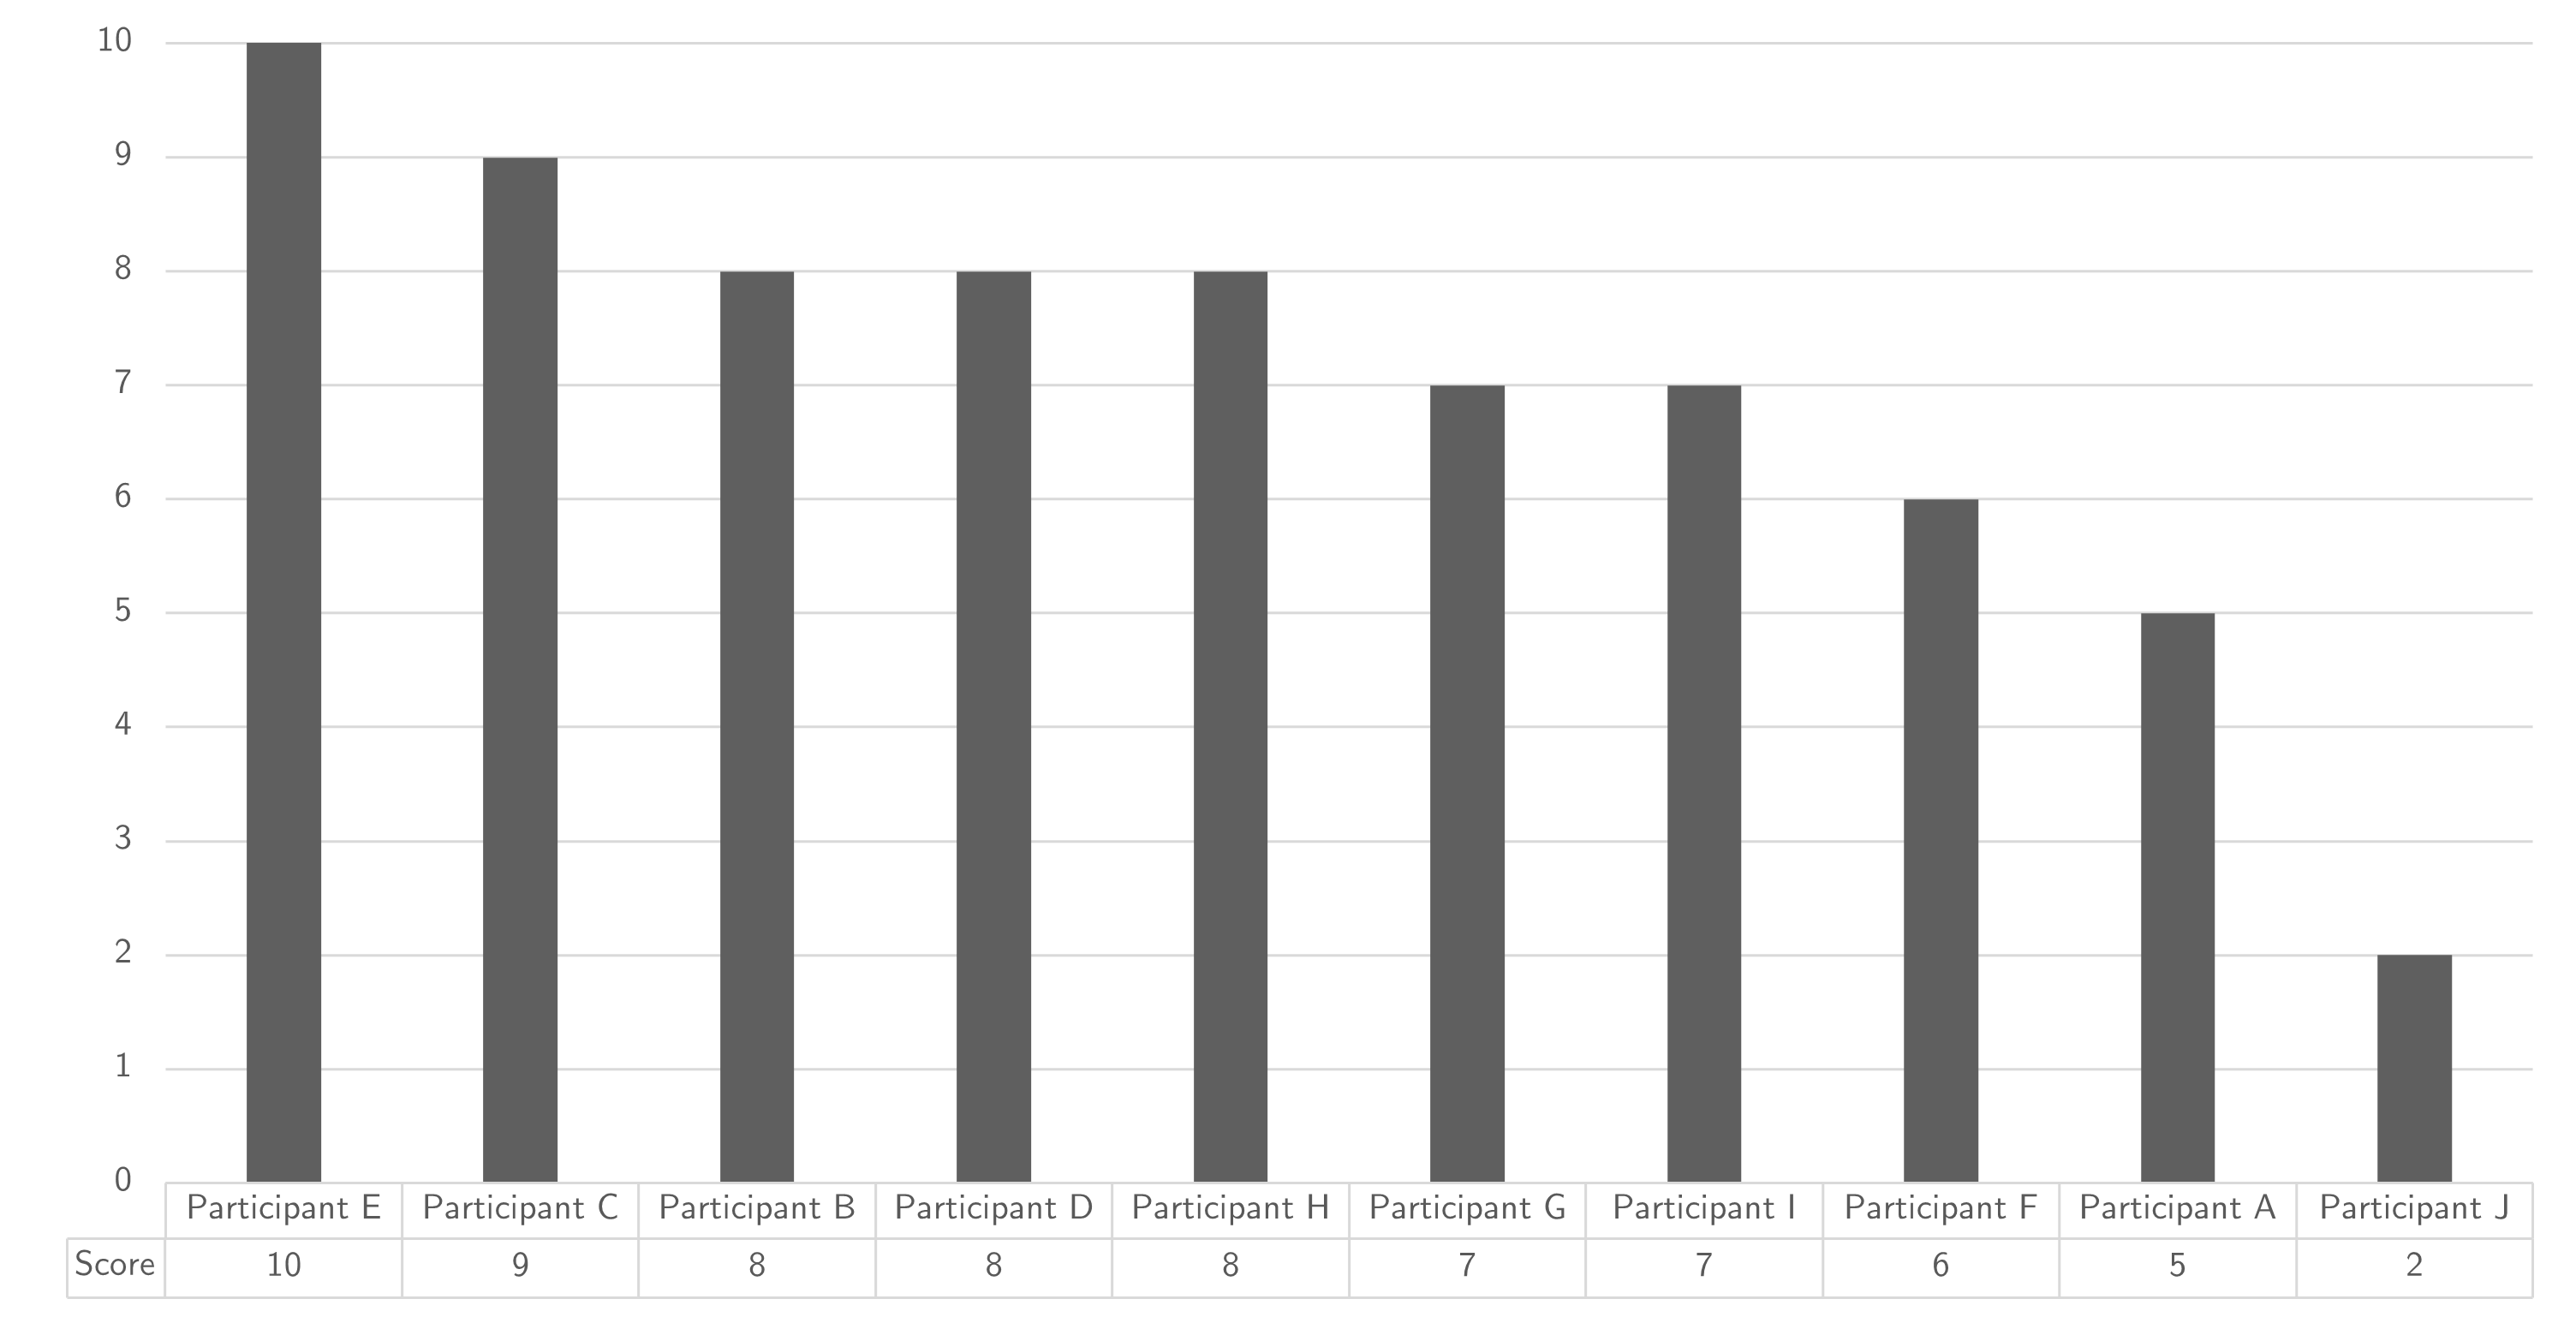
\includegraphics[width=0.9\linewidth]{images/scoreeaholisticsystemsstance}
	\caption[Scoring of EA attribute Holistic (systemic) stance]{Scoring of EA attribute Holistic (systemic) stance}
	\label{fig:appscoringeaholisticsystemsstance}
\end{figure}
\begin{table}[h!]
	\centering
	\begin{tabular}{p{.55\textwidth}ccc}
		\toprule
		\textbf{Attribute} & \textbf{Rating} & \textbf{Variability} & \textbf{Abstains} \\
		\midrule
		Holist (systemic) stance & 7 & 47\% & 0 \\%
		\bottomrule
	\end{tabular}%
	\caption[Scoring of EA attribute Holistic (systemic) stance]{Scoring of EA attribute Holistic (systemic) stance}
	\label{tab:appscoringeaholisticsystemsstance}%
\end{table}%
\newpage
\subsection{Organisational learning}
\begin{figure}[h!]
	\centering
	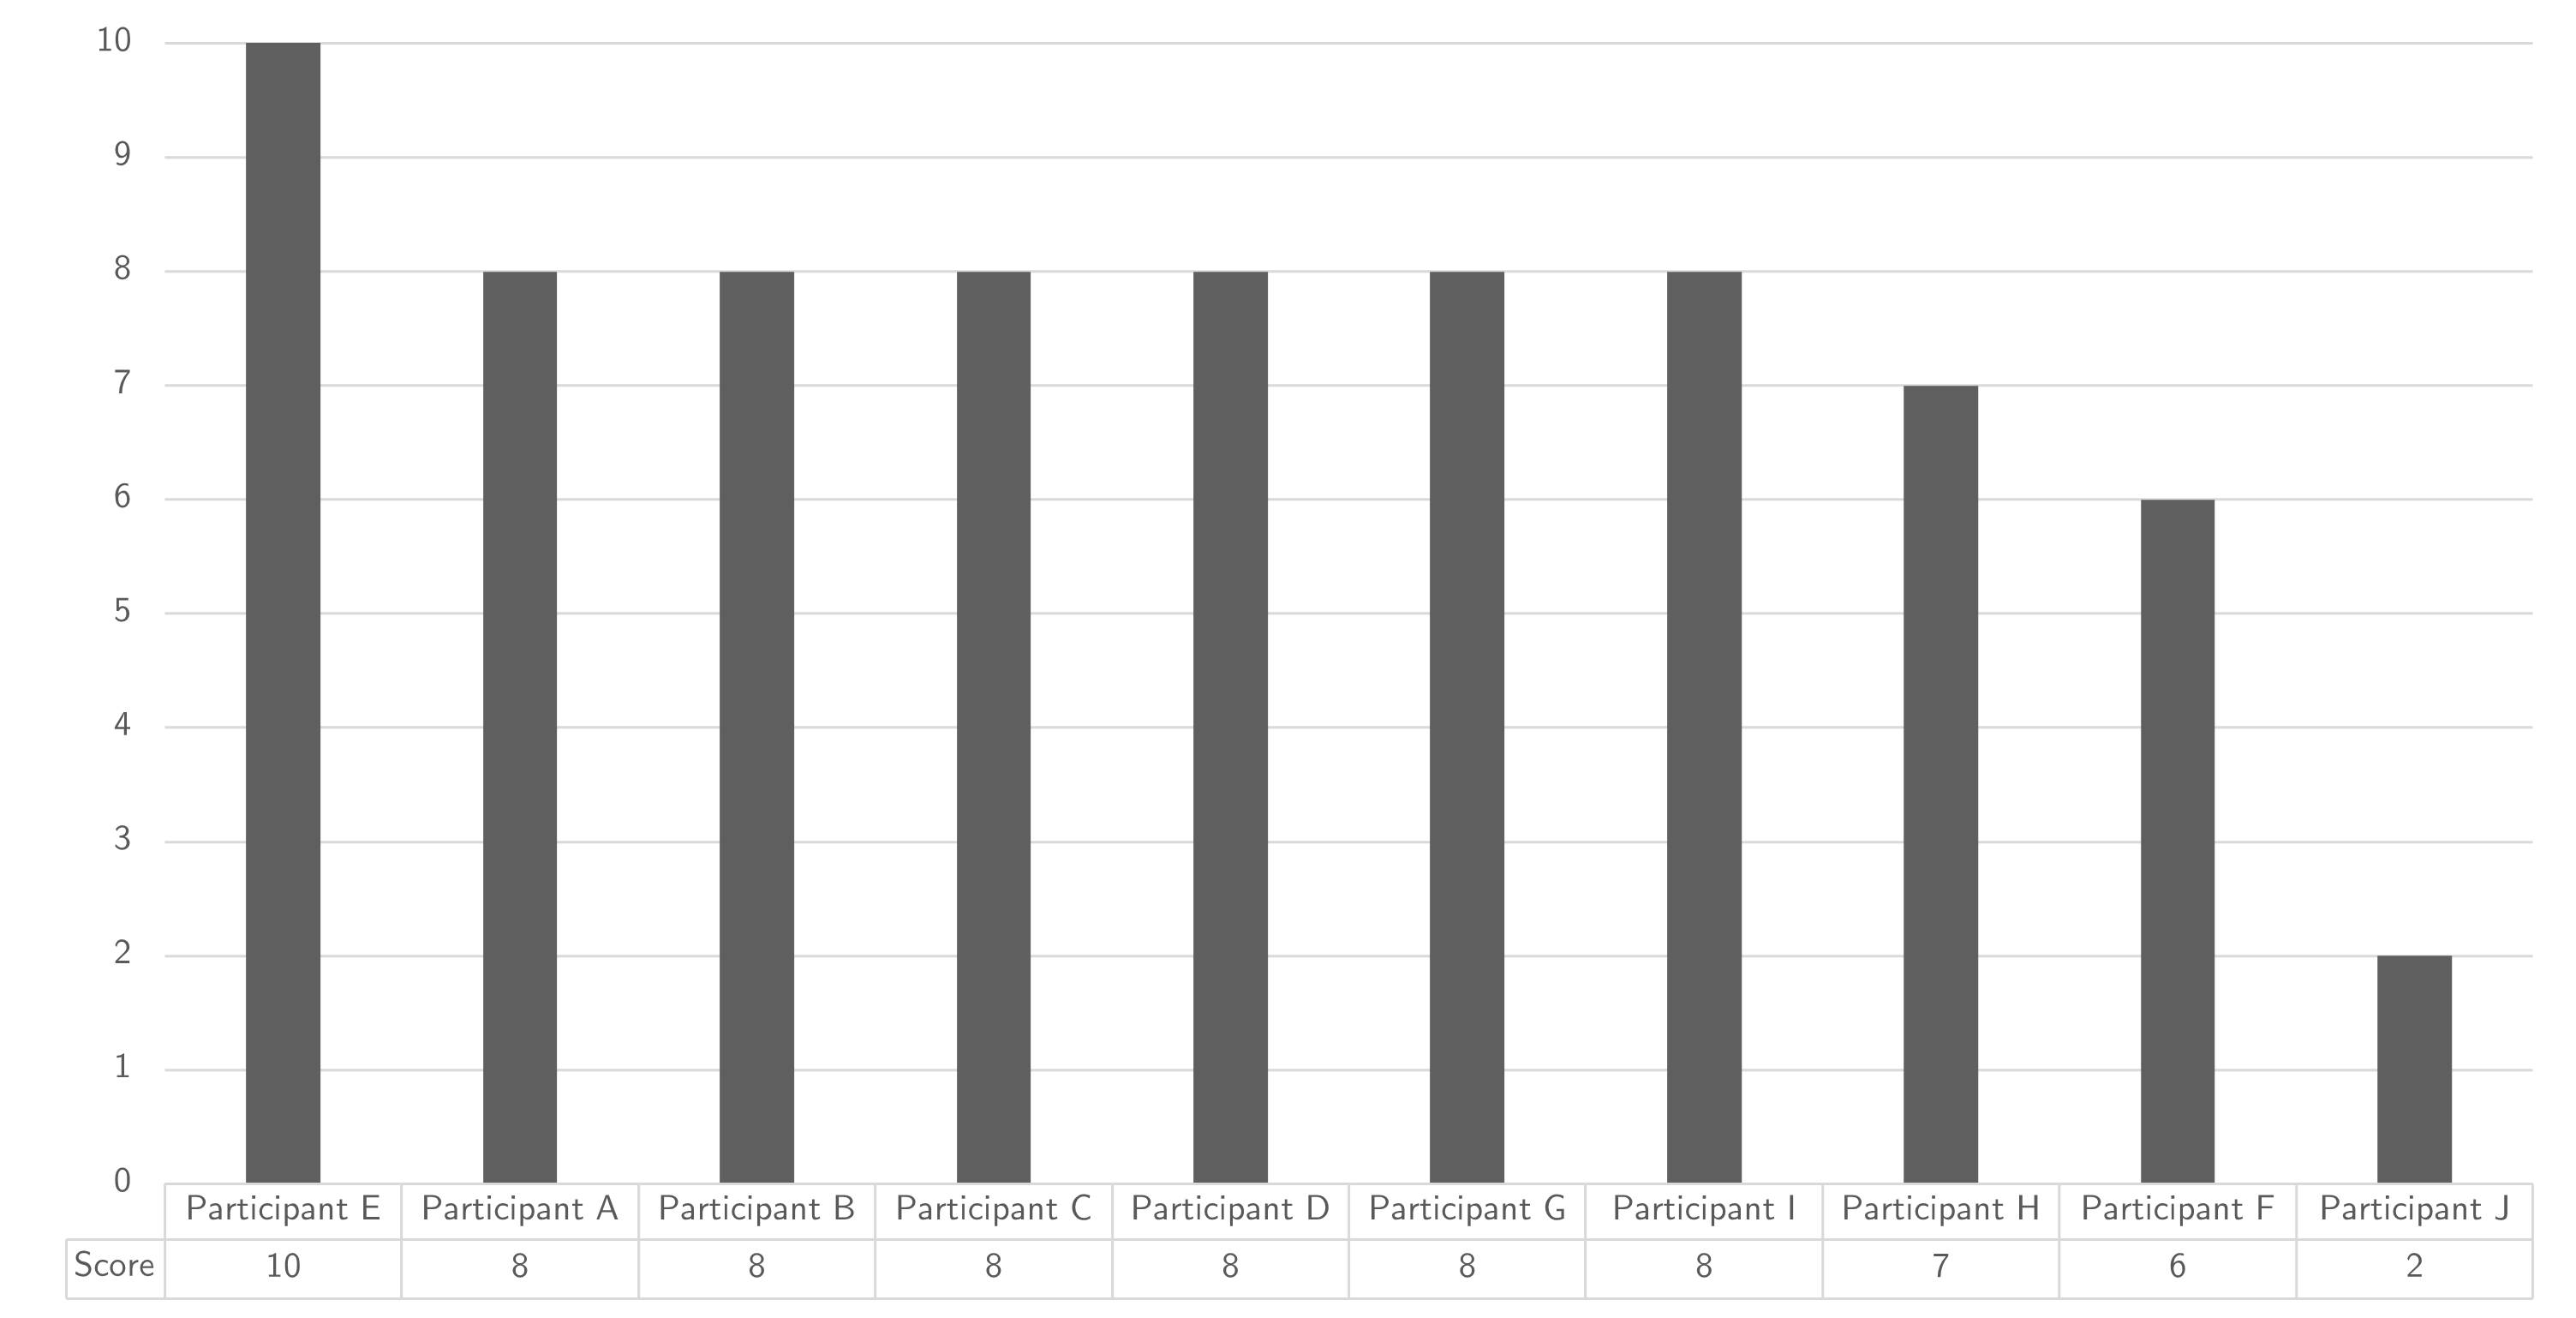
\includegraphics[width=0.9\linewidth]{images/scoreeaorganisationallearning}
	\caption[Scoring of EA attribute Organisational learning]{Scoring of EA attribute Organisational learning}
	\label{fig:appscoringeaorganiationallearning}
\end{figure}
\begin{table}[h!]
	\centering
	\begin{tabular}{p{.55\textwidth}ccc}
		\toprule
		\textbf{Attribute} & \textbf{Rating} & \textbf{Variability} & \textbf{Abstains} \\
		\midrule
		Organisational learning & 7,3 & 44\% & 0 \\%
		\bottomrule
	\end{tabular}%
	\caption[Scoring of EA attribute Organisational learning]{Scoring of EA attribute Organisational learning}
	\label{tab:appscoringeaorganisationallearning}%
\end{table}%
\newpage
\subsection{Environmental learning}
\begin{figure}[h!]
	\centering
	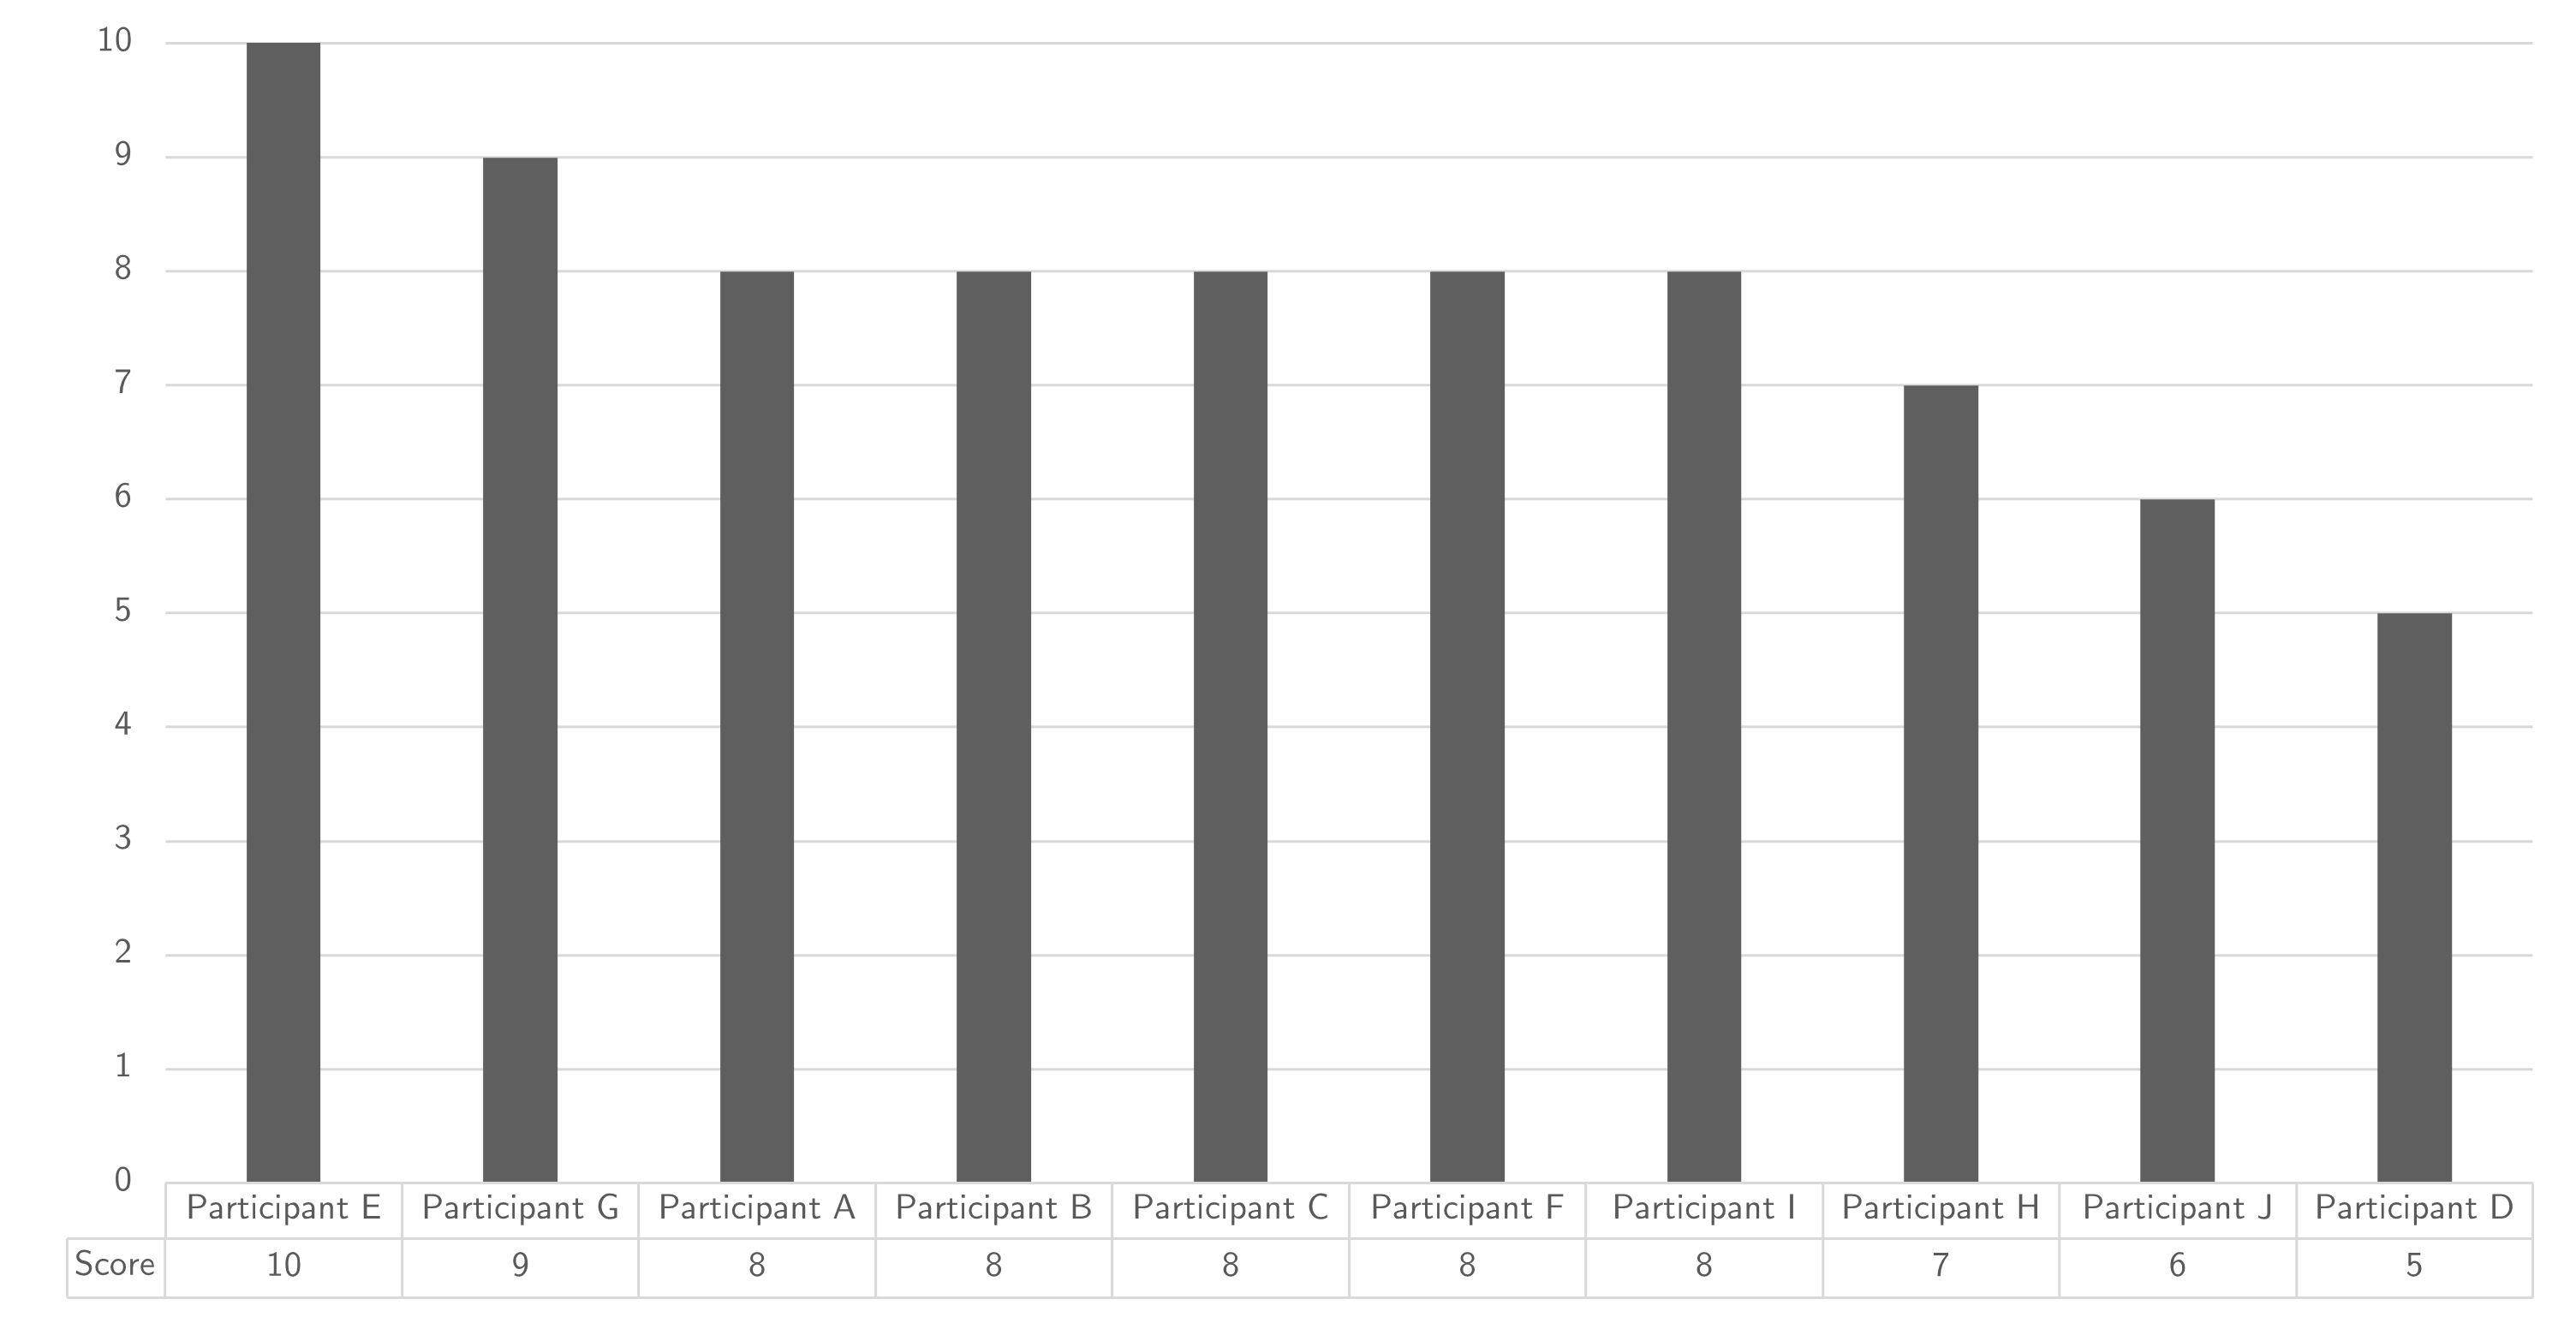
\includegraphics[width=0.9\linewidth]{images/scoreeaenvironmentallearning}
	\caption[Scoring of EA attribute Environmental learning]{Scoring of EA attribute Environmental learning}
	\label{fig:appscoringeaenvironmentallearning}
\end{figure}
\begin{table}[h!]
	\centering
	\begin{tabular}{p{.55\textwidth}ccc}
		\toprule
		\textbf{Attribute} & \textbf{Rating} & \textbf{Variability} & \textbf{Abstains} \\
		\midrule
		Environmental learning & 7,7 & 29\% & 0 \\%
		\bottomrule
	\end{tabular}%
	\caption[Scoring of EA attribute Environmental learning]{Scoring of EA attribute Environmental learning}
	\label{tab:appscoringeaenvironmentallearning}%
\end{table}%
\newpage
\subsection{Intra-organisational coherency}
\begin{figure}[h!]
	\centering
	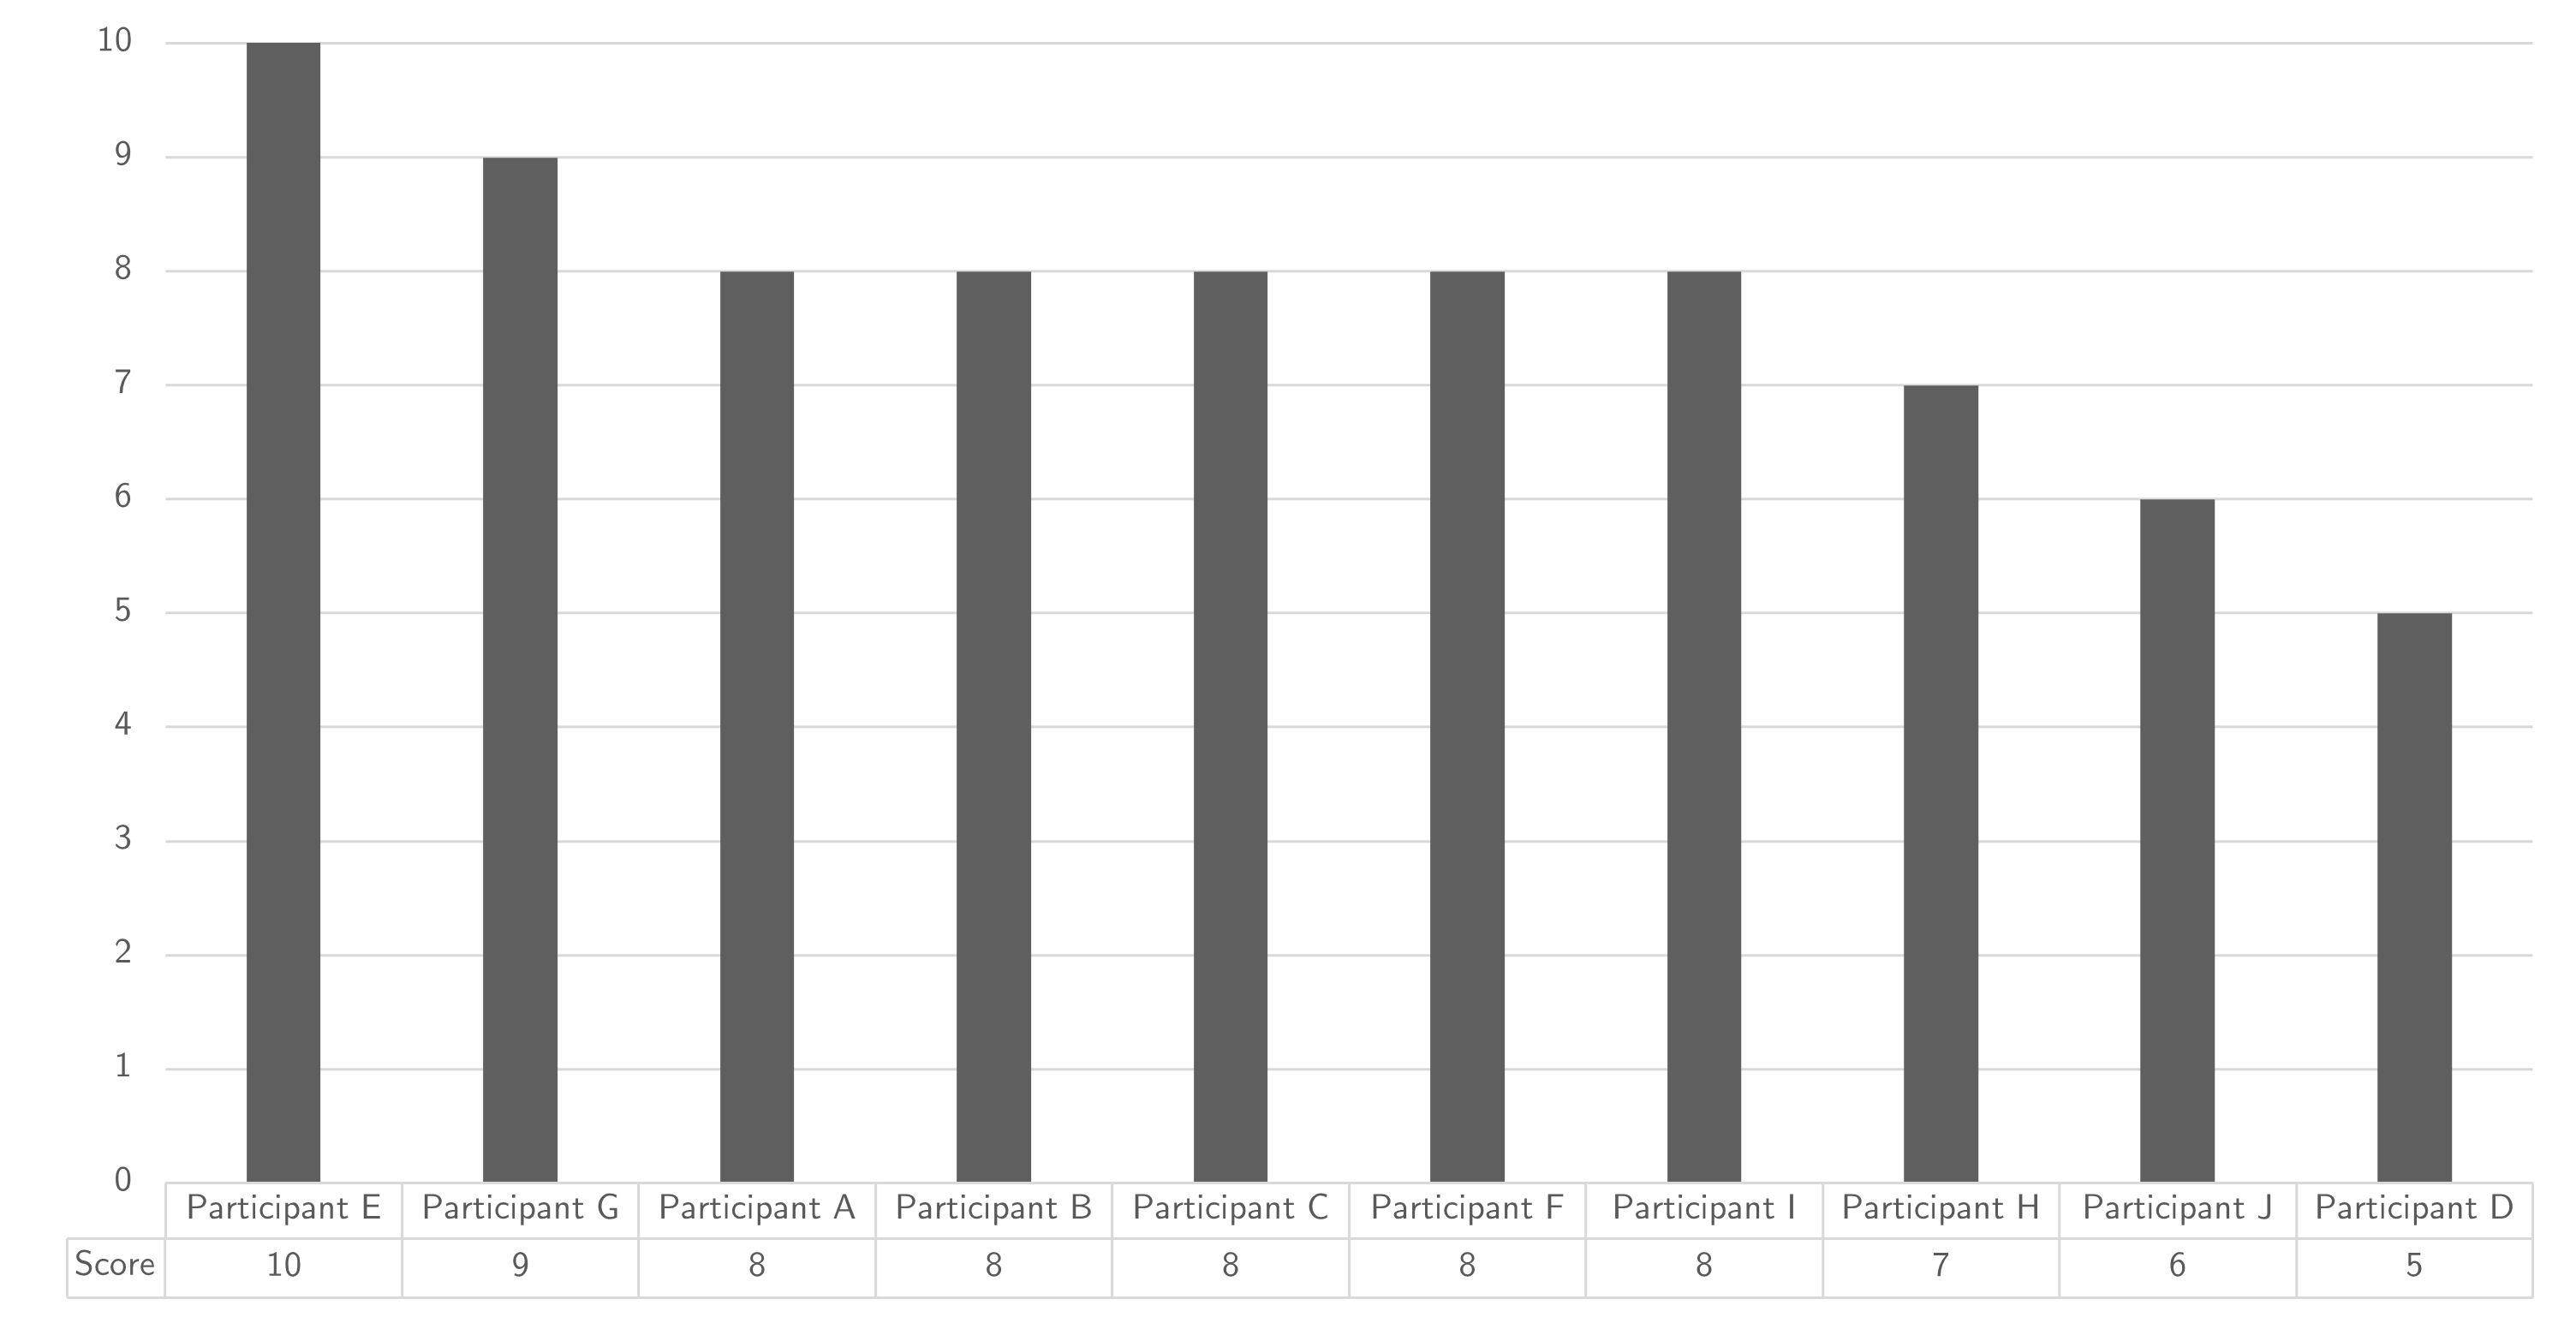
\includegraphics[width=0.9\linewidth]{images/scoreeaintraorganisationalcoherency}
	\caption[Scoring of EA attribute Intra-Organisational coherency]{Scoring of EA attribute Intra-Organisational coherency}
	\label{fig:appscoringeaintraorganisationalcoherency}
\end{figure}
\begin{table}[h!]
	\centering
	\begin{tabular}{p{.55\textwidth}ccc}
		\toprule
		\textbf{Attribute} & \textbf{Rating} & \textbf{Variability} & \textbf{Abstains} \\
		\midrule
		Intra-organisational coherency & 6,4 & 31\% & 0 \\%
		\bottomrule
	\end{tabular}%
	\caption[Scoring of EA attribute Intra-Organisational coherency]{Scoring of EA attribute Intra-Organisational coherency}
	\label{tab:appscoringeaintraorganisationalcoherency}%
\end{table}%
\newpage
\subsection{System-in-Environment Co-Evolution learning}
\begin{figure}[h!]
	\centering
	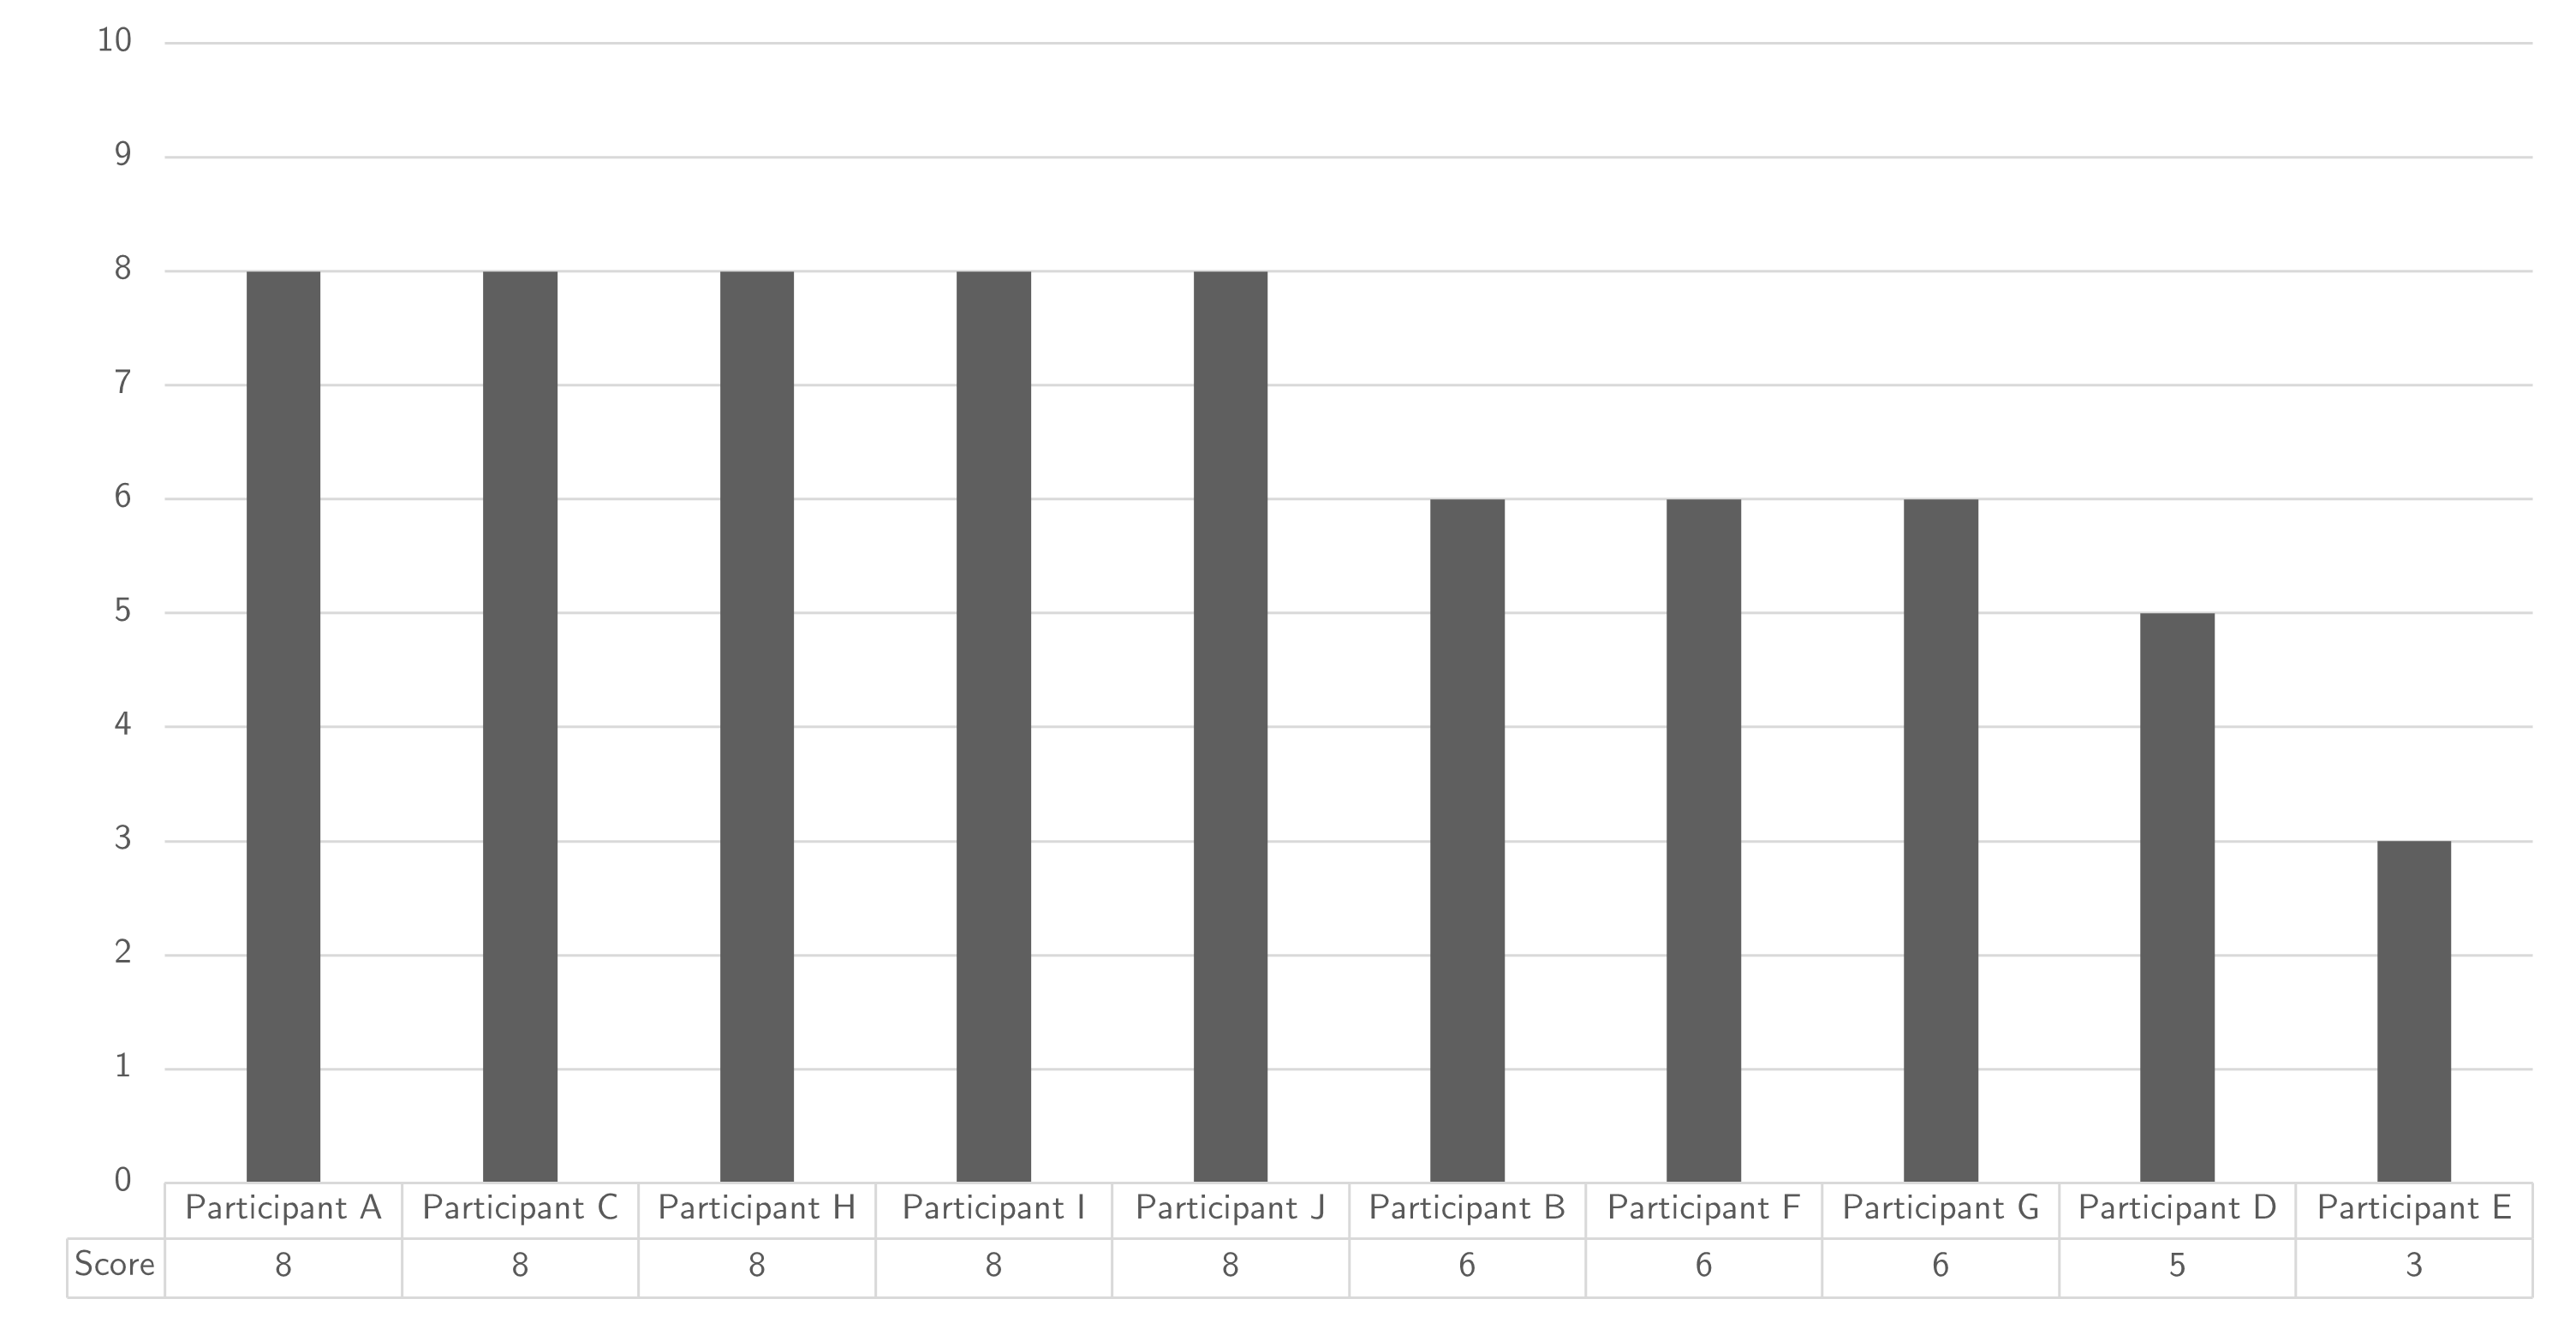
\includegraphics[width=0.9\linewidth]{images/scoreeasysteminenvironmentcoevolution}
	\caption[Scoring of EA attribute System-in-Environment Co-Evolution learning]{Scoring of EA attribute System-in-Environment Co-Evolution learning}
	\label{fig:appscoringeasysteminenvironmentcoevolutionlearning}
\end{figure}
\begin{table}[h!]
	\centering
	\begin{tabular}{p{.55\textwidth}ccc}
		\toprule
		\textbf{Attribute} & \textbf{Rating} & \textbf{Variability} & \textbf{Abstains} \\
		\midrule
		System-in-environment coevolution learning & 6,6 & 36\% & 0 \\%
		\bottomrule
	\end{tabular}%
	\caption[Scoring of EA attribute System-in-Environment Co-Evolution learning]{Scoring of EA attribute System-in-Environment Co-Evolution learning}
	\label{tab:appscoringeasysteminenvironmentcoevolutionlearning}%
\end{table}%
\newpage
\subsection{Adapt to business language}
\begin{figure}[h!]
	\centering
	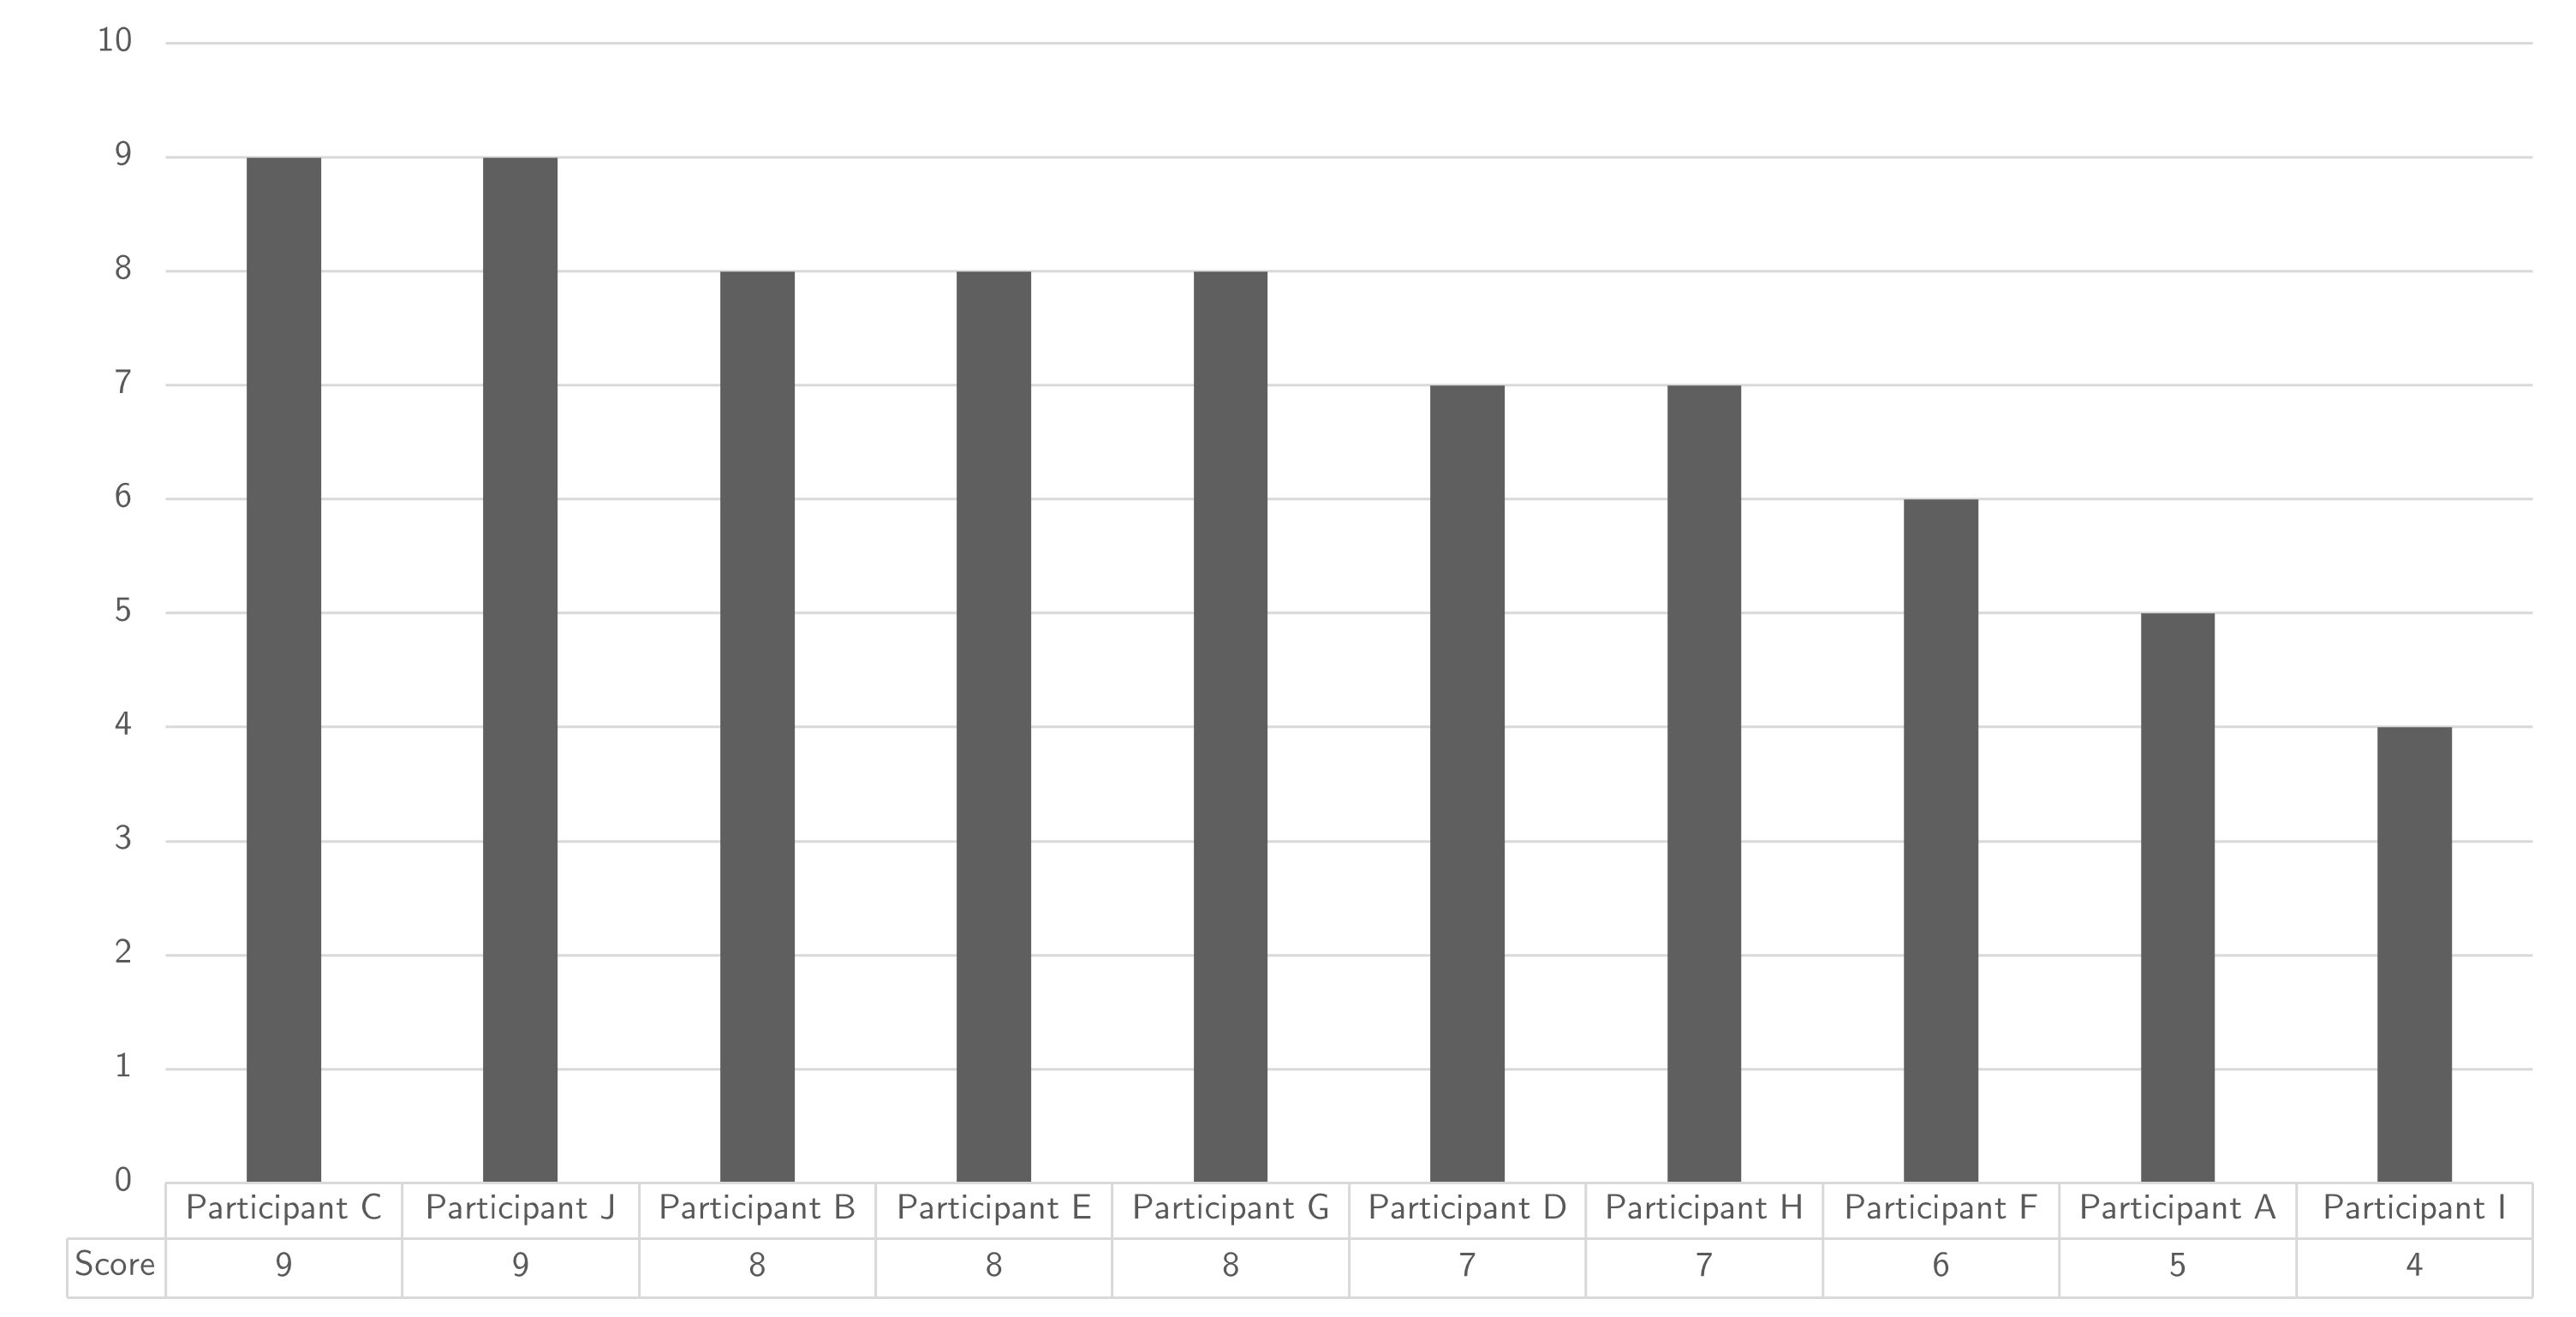
\includegraphics[width=0.9\linewidth]{images/scoreeaadapttobusinesslanguage}
	\caption[Scoring of EA attribute adapt to business language]{Scoring of EA attribute adapt to business language}
	\label{fig:appscoringeaadapttobusinesslanguage}
\end{figure}
\begin{table}[h!]
	\centering
	\begin{tabular}{p{.55\textwidth}ccc}
		\toprule
		\textbf{Attribute} & \textbf{Rating} & \textbf{Variability} & \textbf{Abstains} \\
		\midrule
		Adapt to business language & 7,1 & 35\% & 0 \\%
		\bottomrule
	\end{tabular}%
	\caption[Scoring of EA attribute adapt to business language]{Scoring of EA attribute adapt to business language}
	\label{tab:appscoringeaadapttobusinesslanguage}%
\end{table}%
\newpage
\subsection{Agile Enterprise}
\begin{figure}[h!]
	\centering
	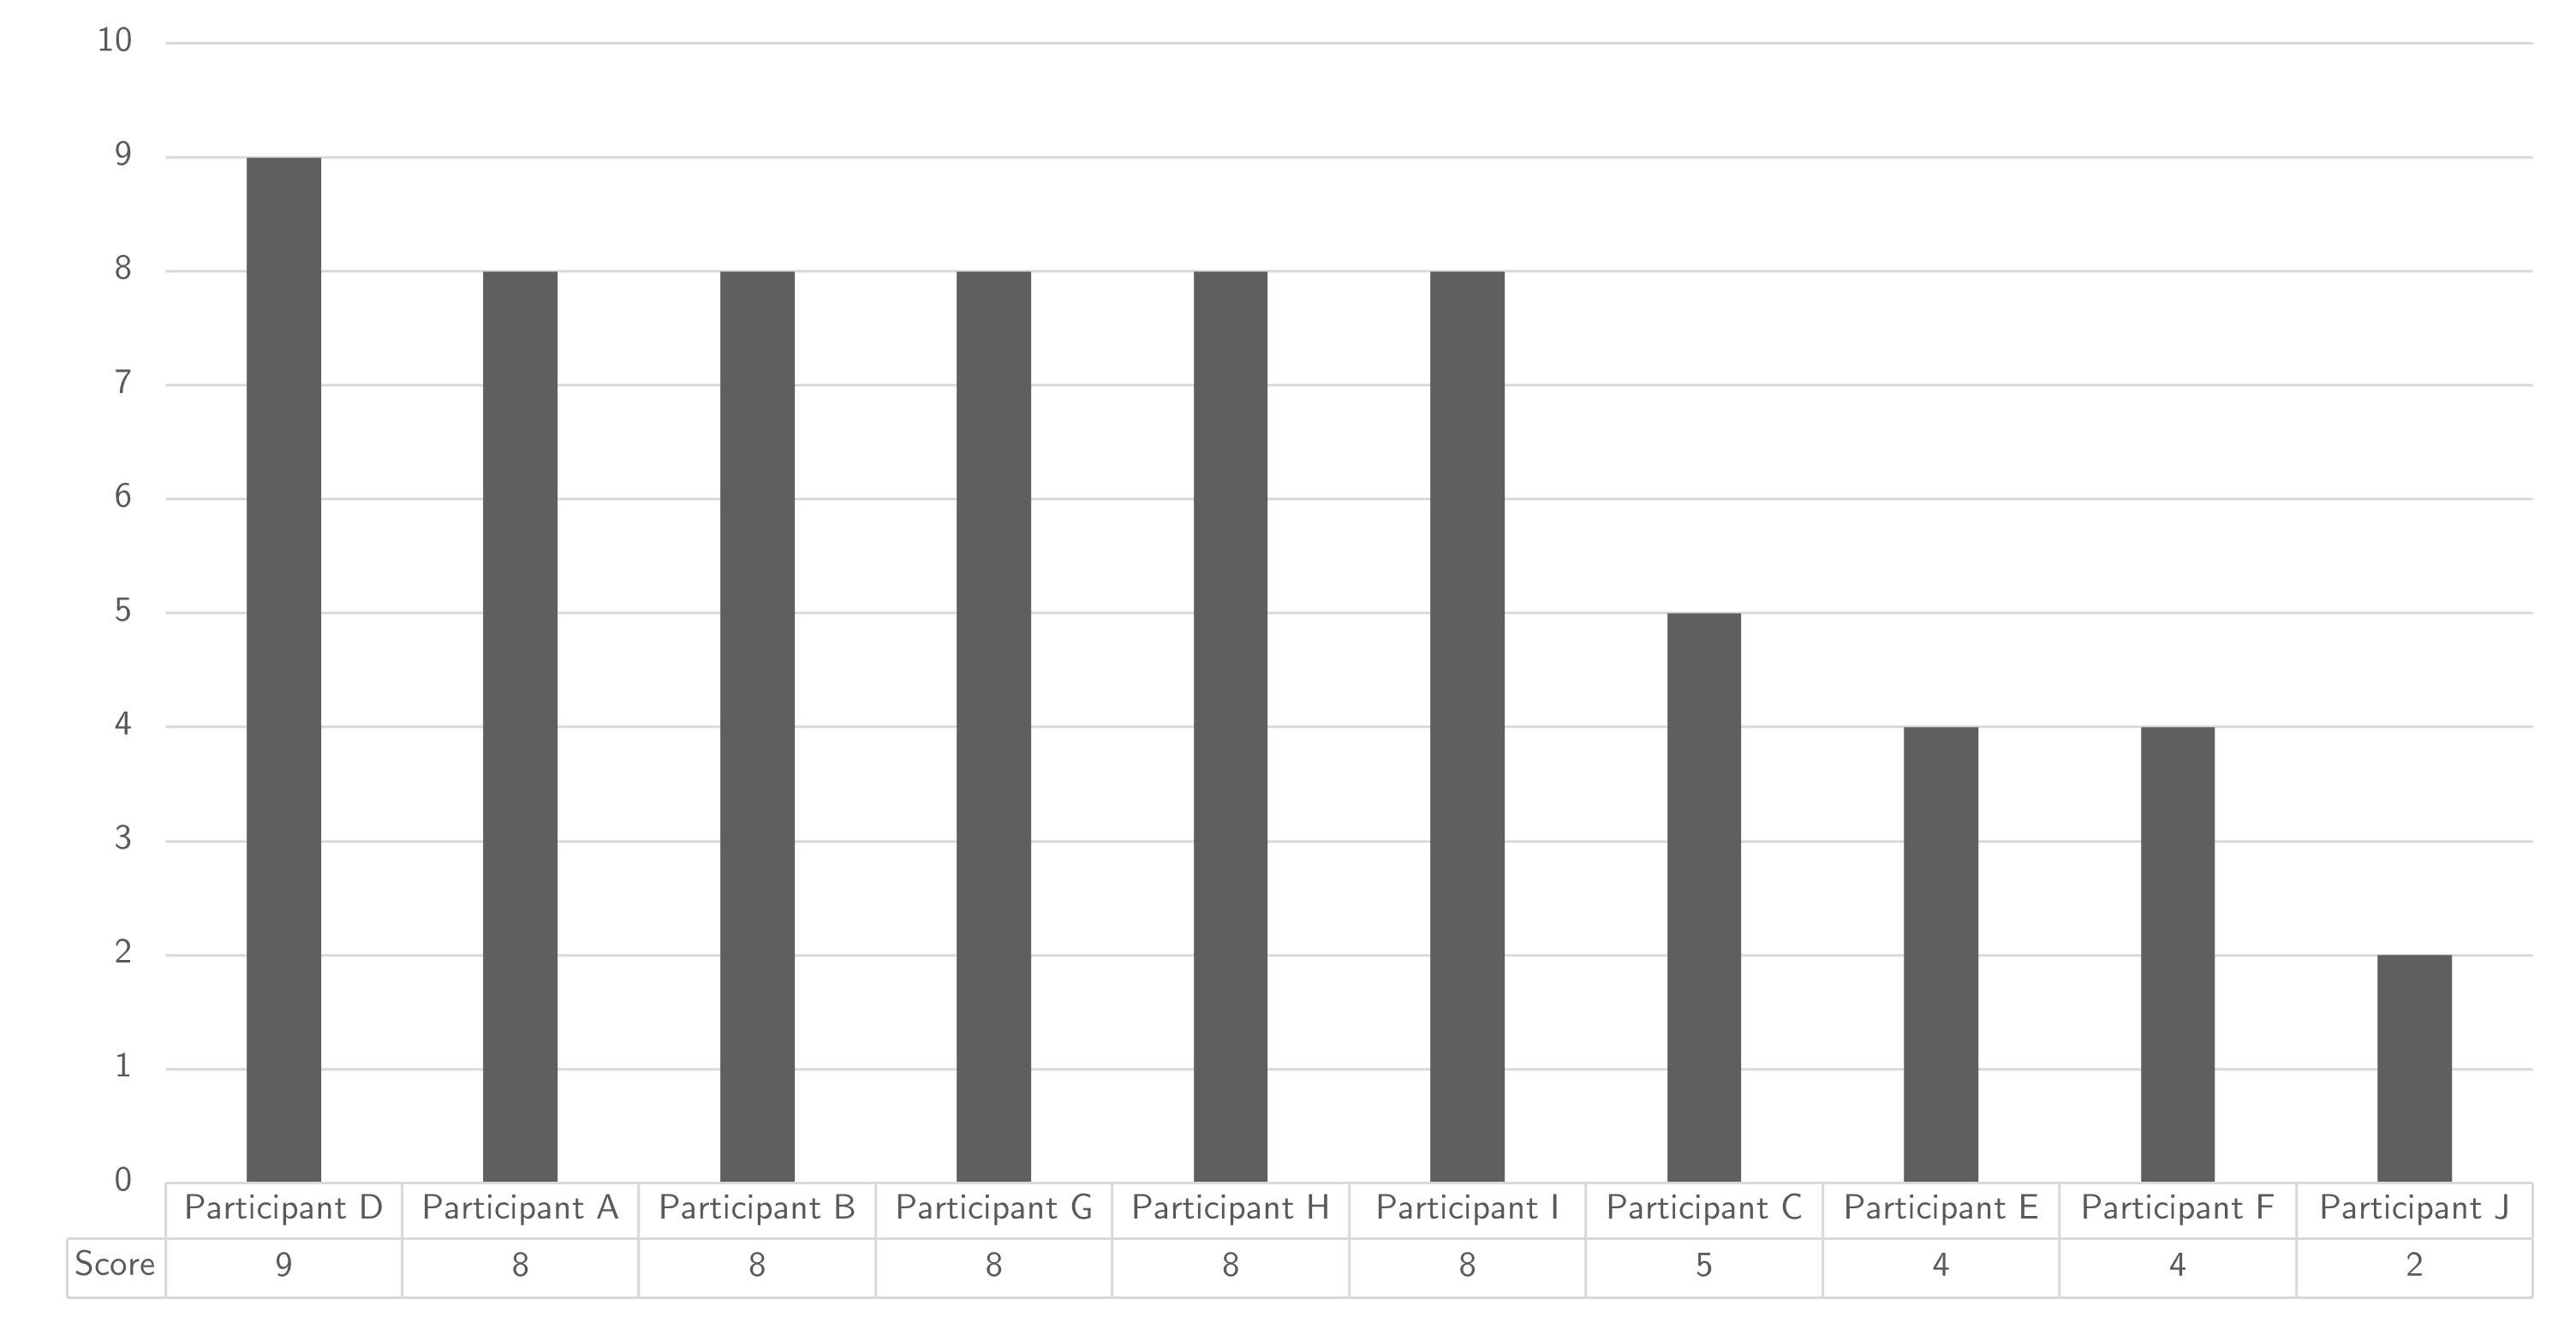
\includegraphics[width=0.9\linewidth]{images/scoreeaagileenterprise}
	\caption[Scoring of EA attribute Agile Enterprise]{Scoring of EA attribute Agile Enterprise}
	\label{fig:appscoringeaagileneterprise}
\end{figure}
\begin{table}[h!]
	\centering
	\begin{tabular}{p{.55\textwidth}ccc}
		\toprule
		\textbf{Attribute} & \textbf{Rating} & \textbf{Variability} & \textbf{Abstains} \\
		\midrule
		Agile Enterprise & 6,4 & 50\% & 0 \\%
		\bottomrule
	\end{tabular}%
	\caption[Scoring of EA attribute Agile Enterprise]{Scoring of EA attribute Agile Enterprise}
	\label{tab:appscoringeaagileenterprise}%
\end{table}%
\newpage
\subsection{Real Time Trust}
\begin{figure}[h!]
	\centering
	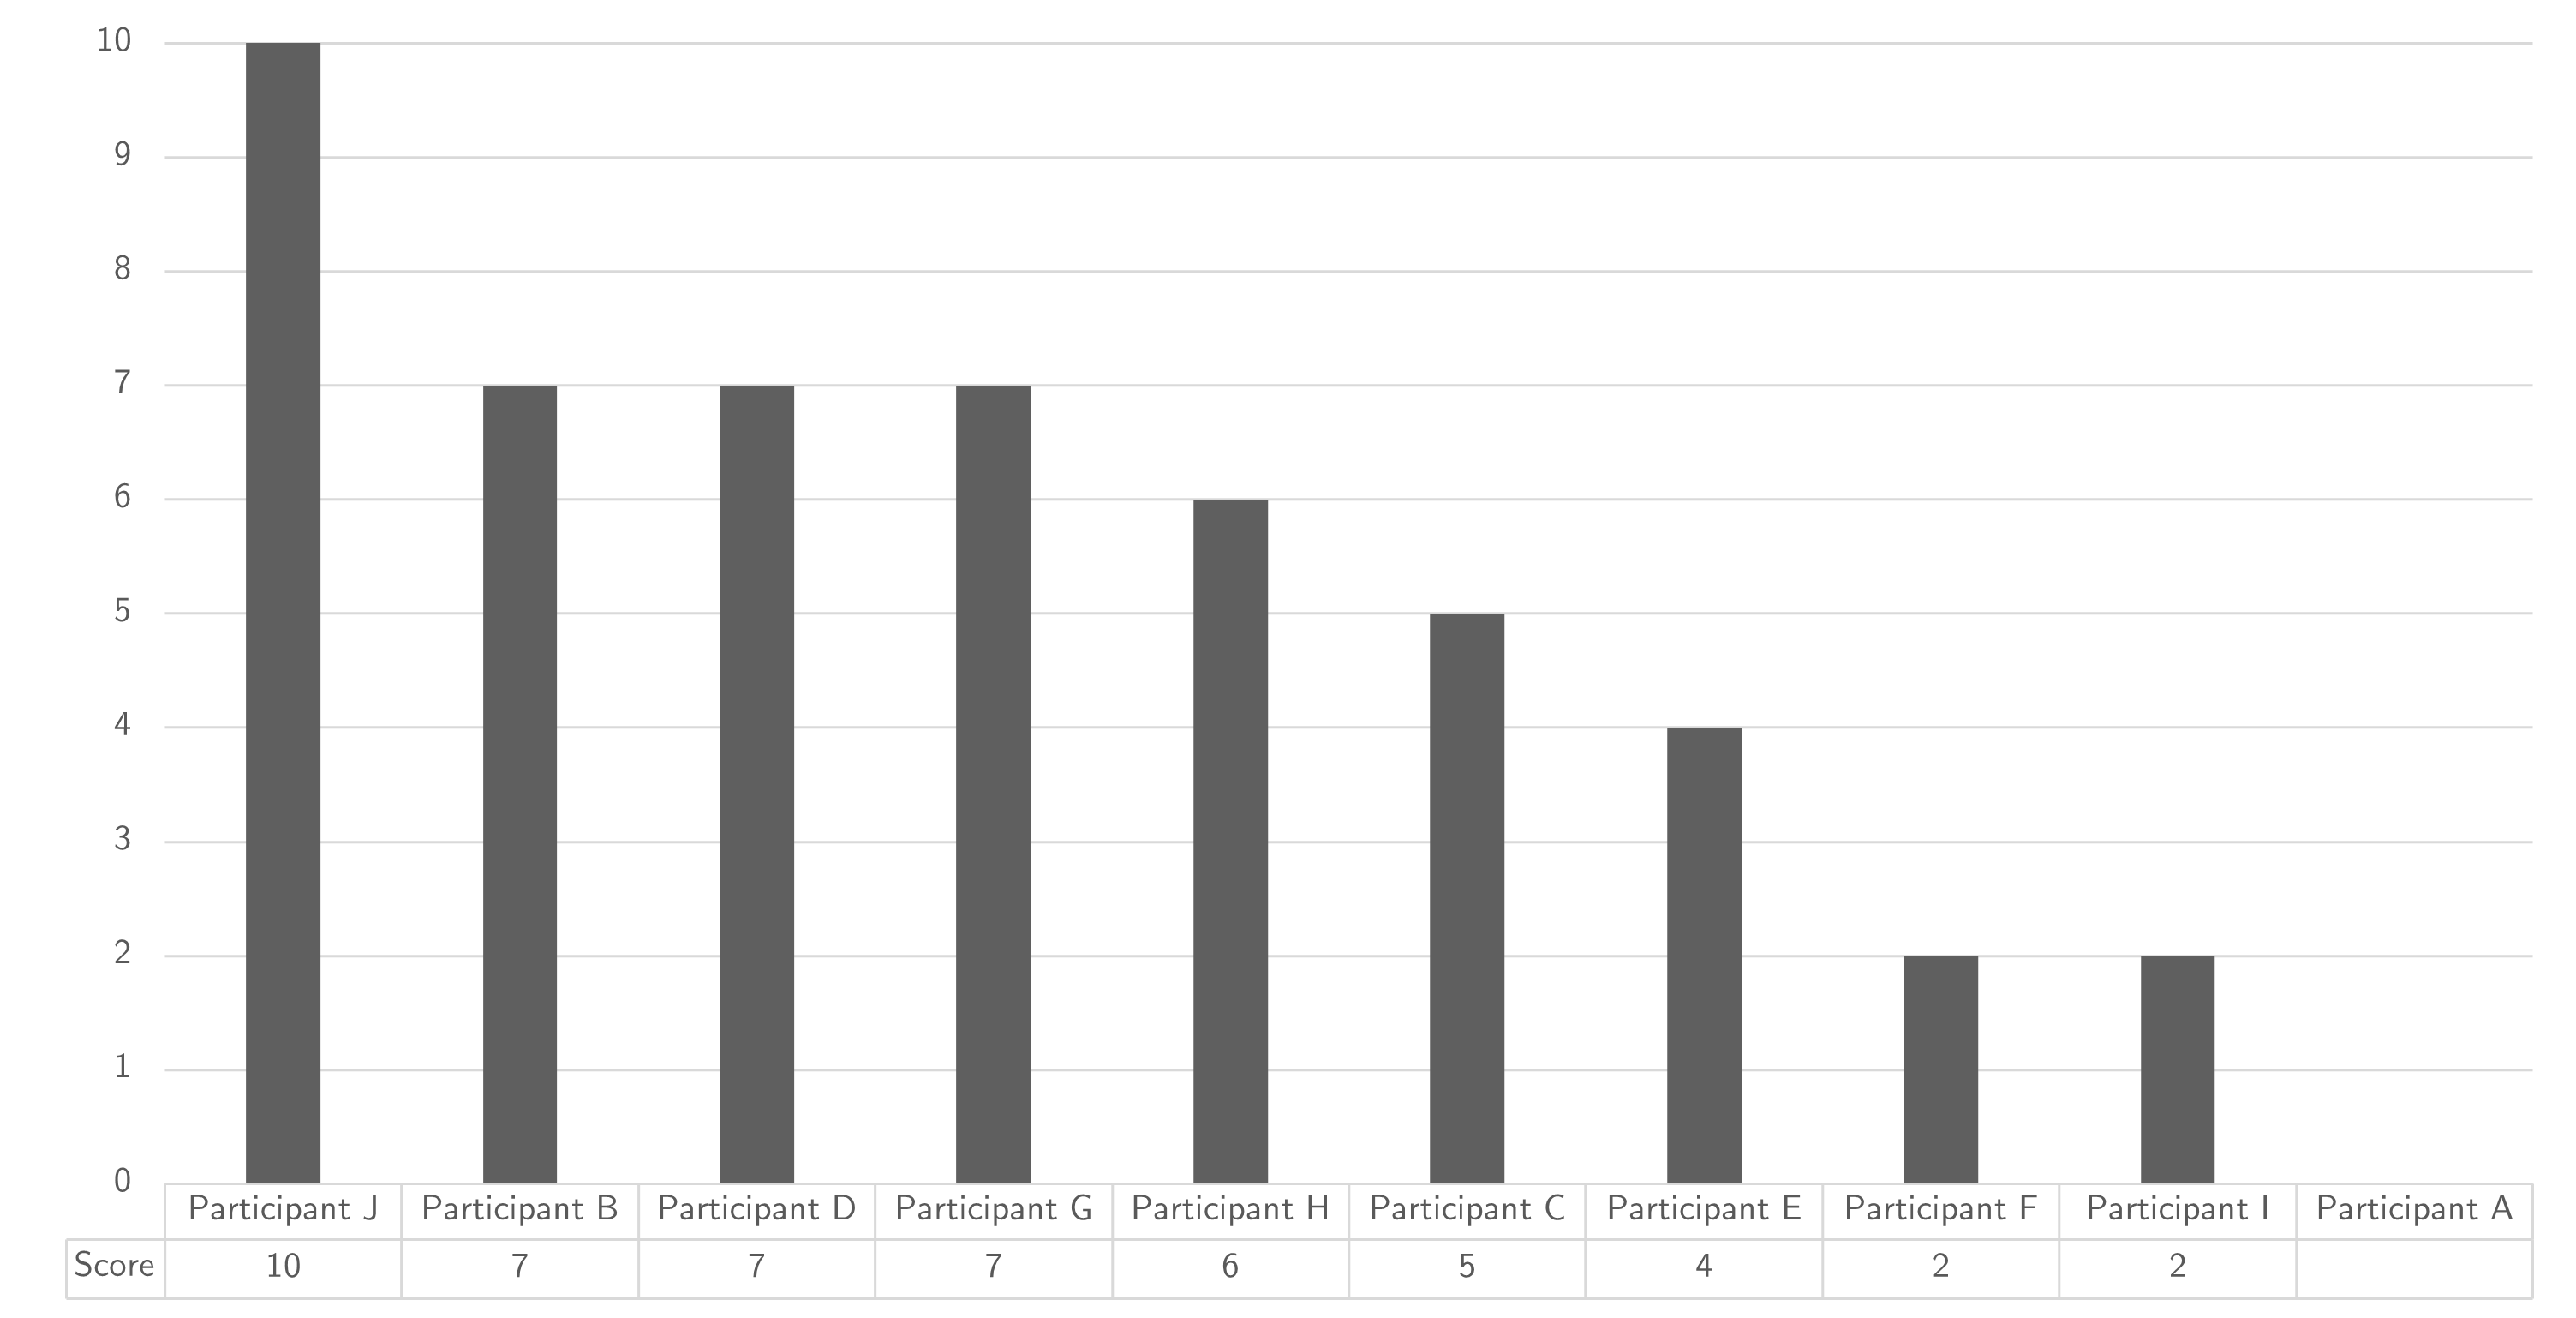
\includegraphics[width=0.9\linewidth]{images/scoreearealtimetrust}
	\caption[Scoring of EA attribute Real Time Trust]{Scoring of EA attribute Real Time Trust}
	\label{fig:appscoringearealtimetrust}
\end{figure}
\begin{table}[h!]
	\centering
	\begin{tabular}{p{.55\textwidth}ccc}
		\toprule
		\textbf{Attribute} & \textbf{Rating} & \textbf{Variability} & \textbf{Abstains} \\
		\midrule
		Real Time Trust (Policy \& Attribute based) & 5,6 & 54\% & 1 \\%
		\bottomrule
	\end{tabular}%
	\caption[Scoring of EA attribute Real Time Trust]{Scoring of EA attribute Real Time Trust}
	\label{tab:appscoringearealtimetrust}%
\end{table}%
\newpage
\subsection{Foster Dialogue}
\begin{figure}[h!]
	\centering
	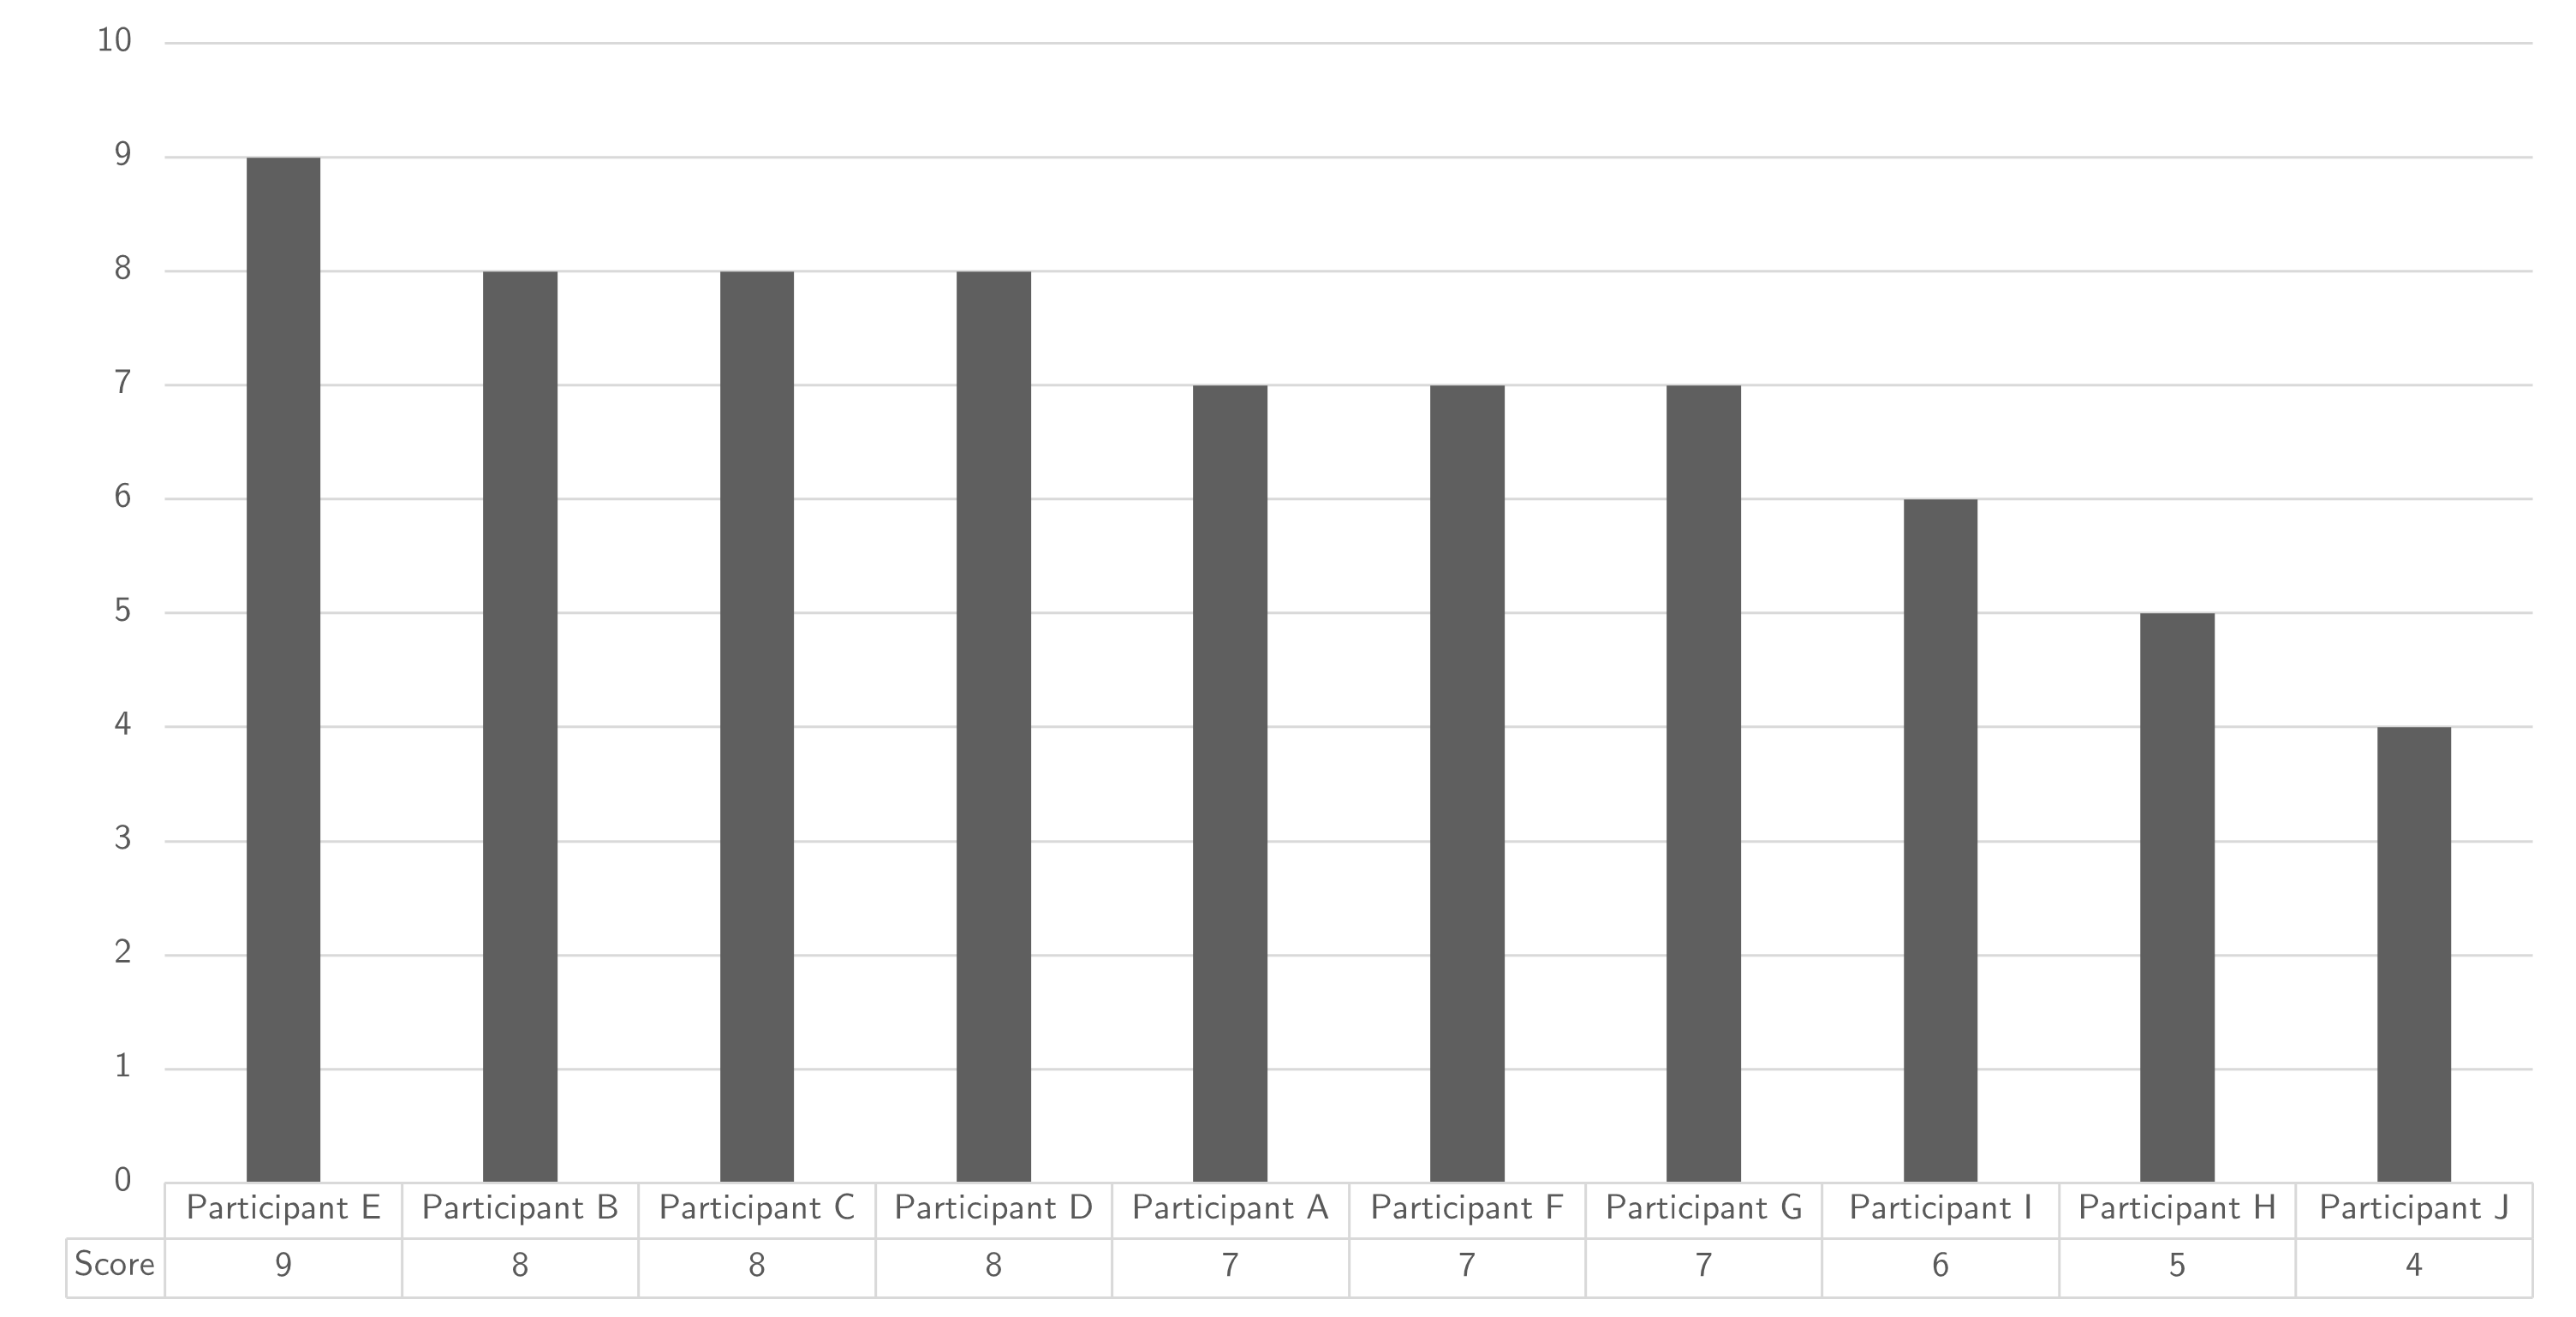
\includegraphics[width=0.9\linewidth]{images/scoreeafosterdialogue}
	\caption[Scoring of EA attribute Foster Dialogue]{Scoring of EA attribute Foster Dialogue}
	\label{fig:appscoringeafosterdialogue}
\end{figure}
\begin{table}[h!]
	\centering
	\begin{tabular}{p{.55\textwidth}ccc}
		\toprule
		\textbf{Attribute} & \textbf{Rating} & \textbf{Variability} & \textbf{Abstains} \\
		\midrule
		Foster Dialogue & 6,9 & 32\% & 0 \\%
		\bottomrule
	\end{tabular}%
	\caption[Scoring of EA attribute Foster Dialogue]{Scoring of EA attribute Foster Dialogue}
	\label{tab:appscoringeafosterdialogue}%
\end{table}%
\newpage
\subsection{Validation}
\begin{figure}[h!]
	\centering
	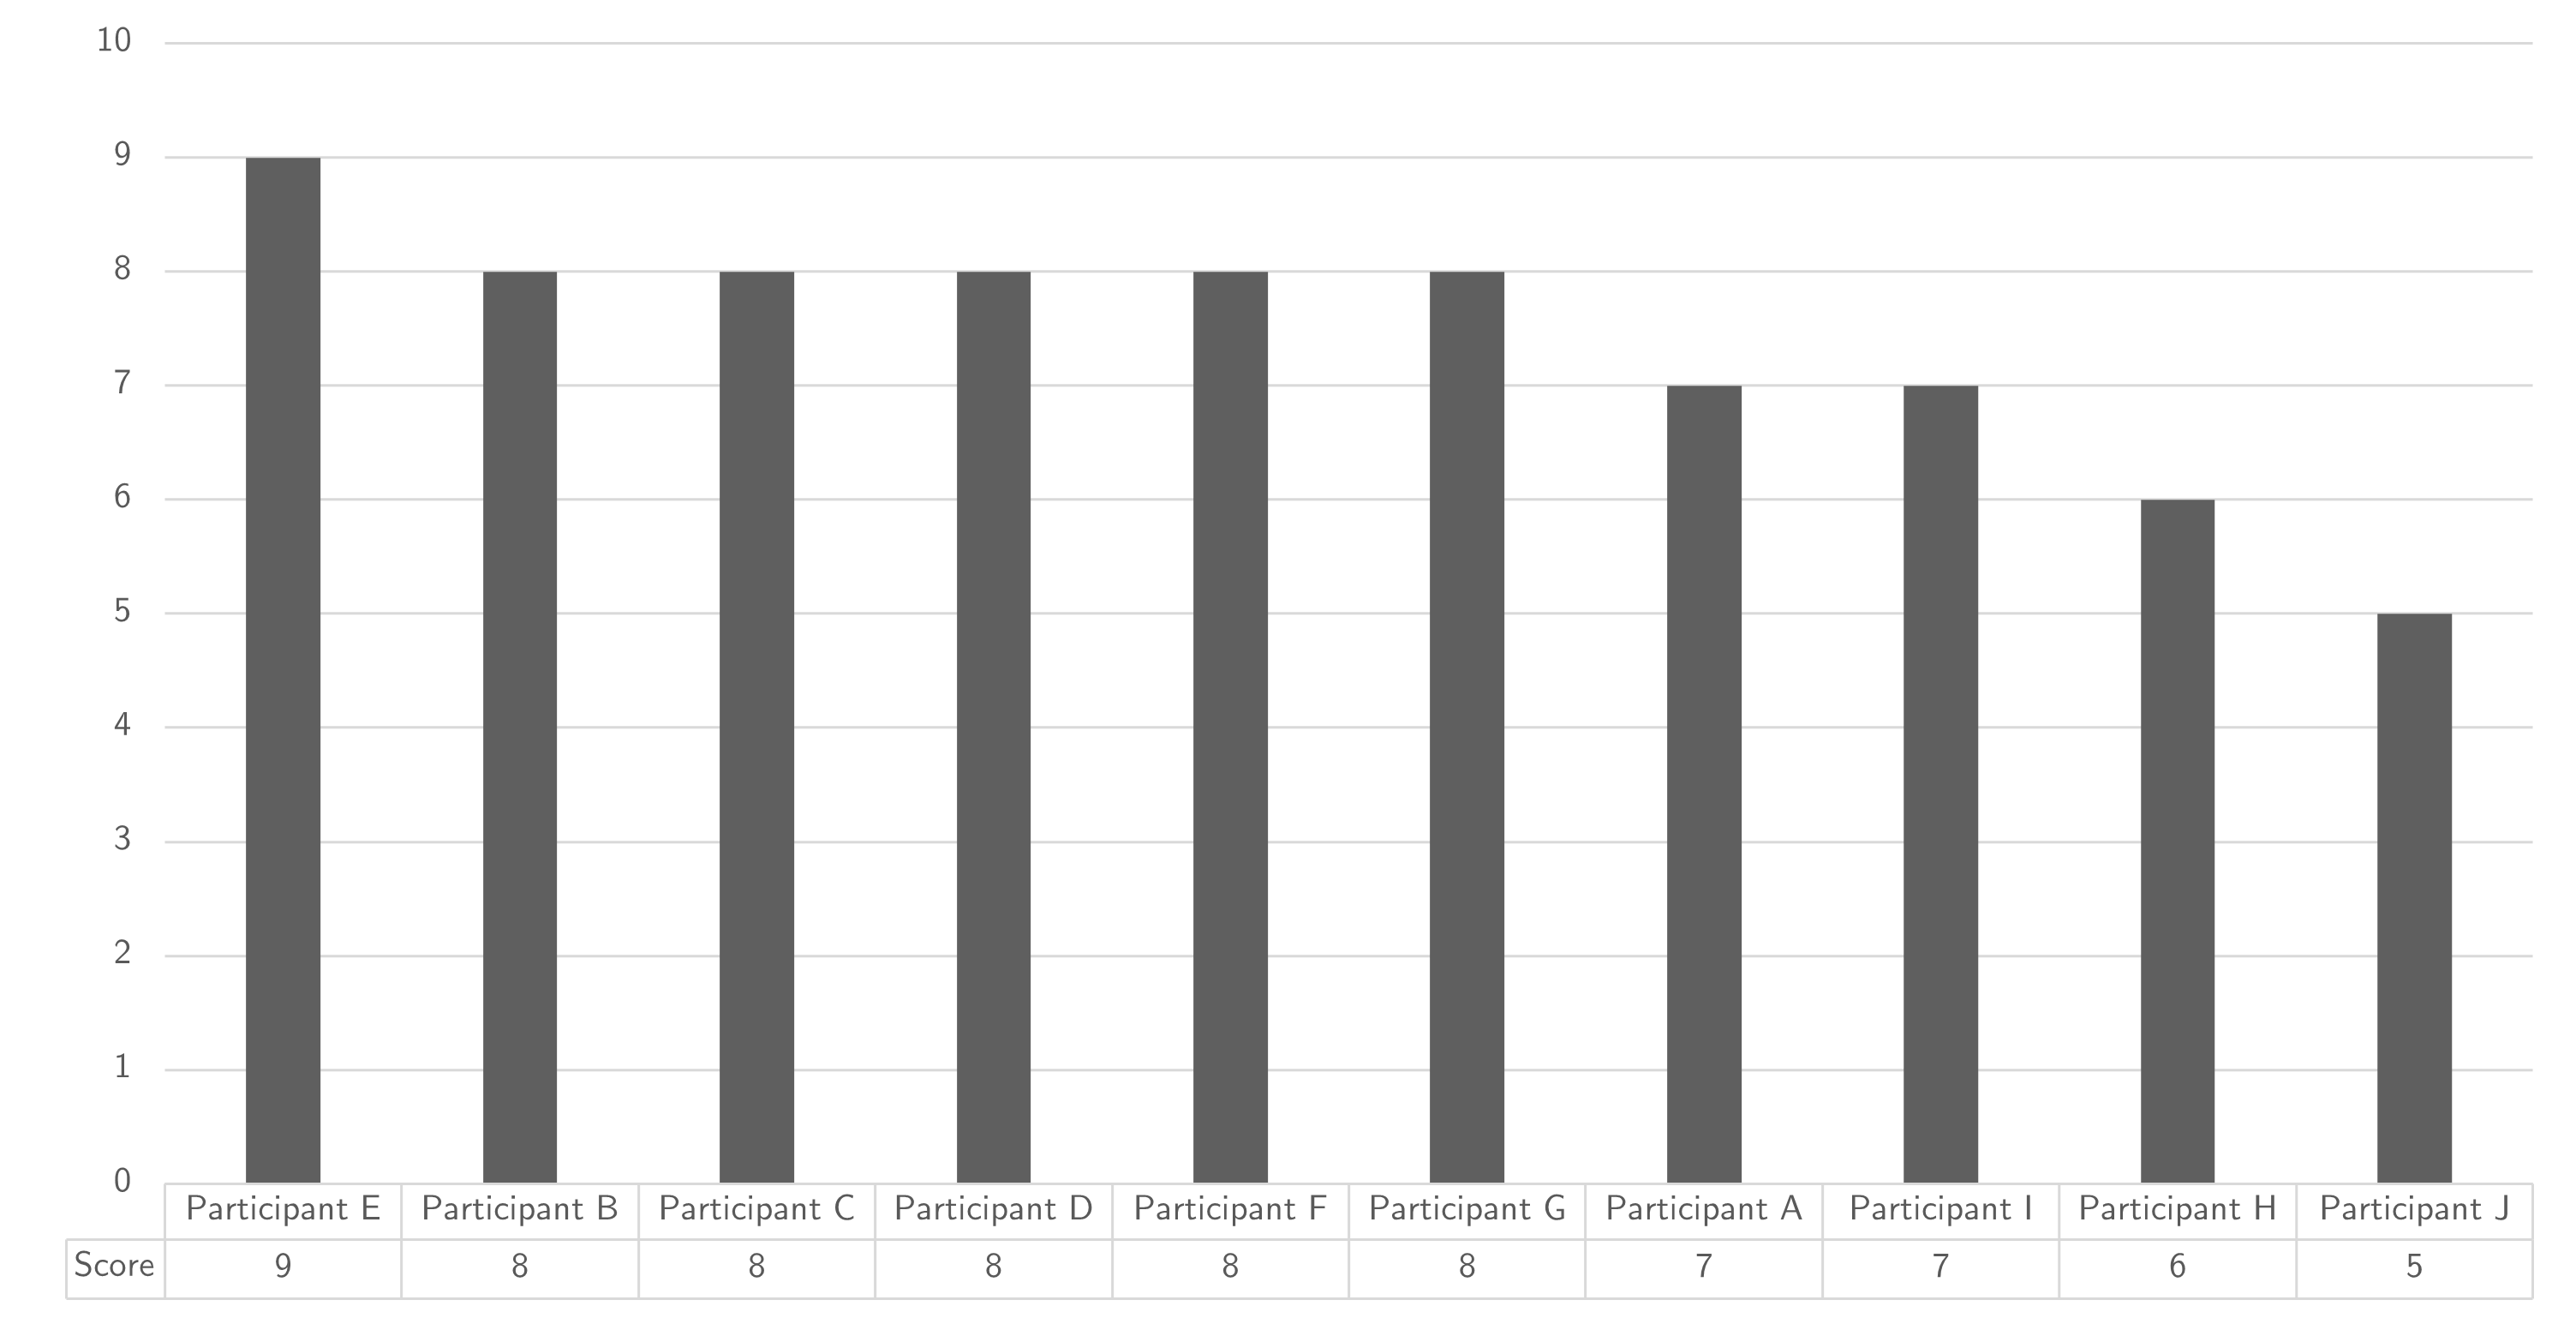
\includegraphics[width=0.9\linewidth]{images/scoreeavalidation}
	\caption[Scoring of EA attribute Validation]{Scoring of EA attribute Validation}
	\label{fig:appscoringeavalidation}
\end{figure}
\begin{table}[h!]
	\centering
	\begin{tabular}{p{.55\textwidth}ccc}
		\toprule
		\textbf{Attribute} & \textbf{Rating} & \textbf{Variability} & \textbf{Abstains} \\
		\midrule
		Validation & 7,4 & 24\% & 0 \\%
		\bottomrule
	\end{tabular}%
	\caption[Scoring of EA attribute Validation]{Scoring of EA attribute Validation}
	\label{tab:appscoringeavalidation}%
\end{table}%
\newpage
\subsection{Always fitting Enterprise Architecture}
\begin{figure}[h!]
	\centering
	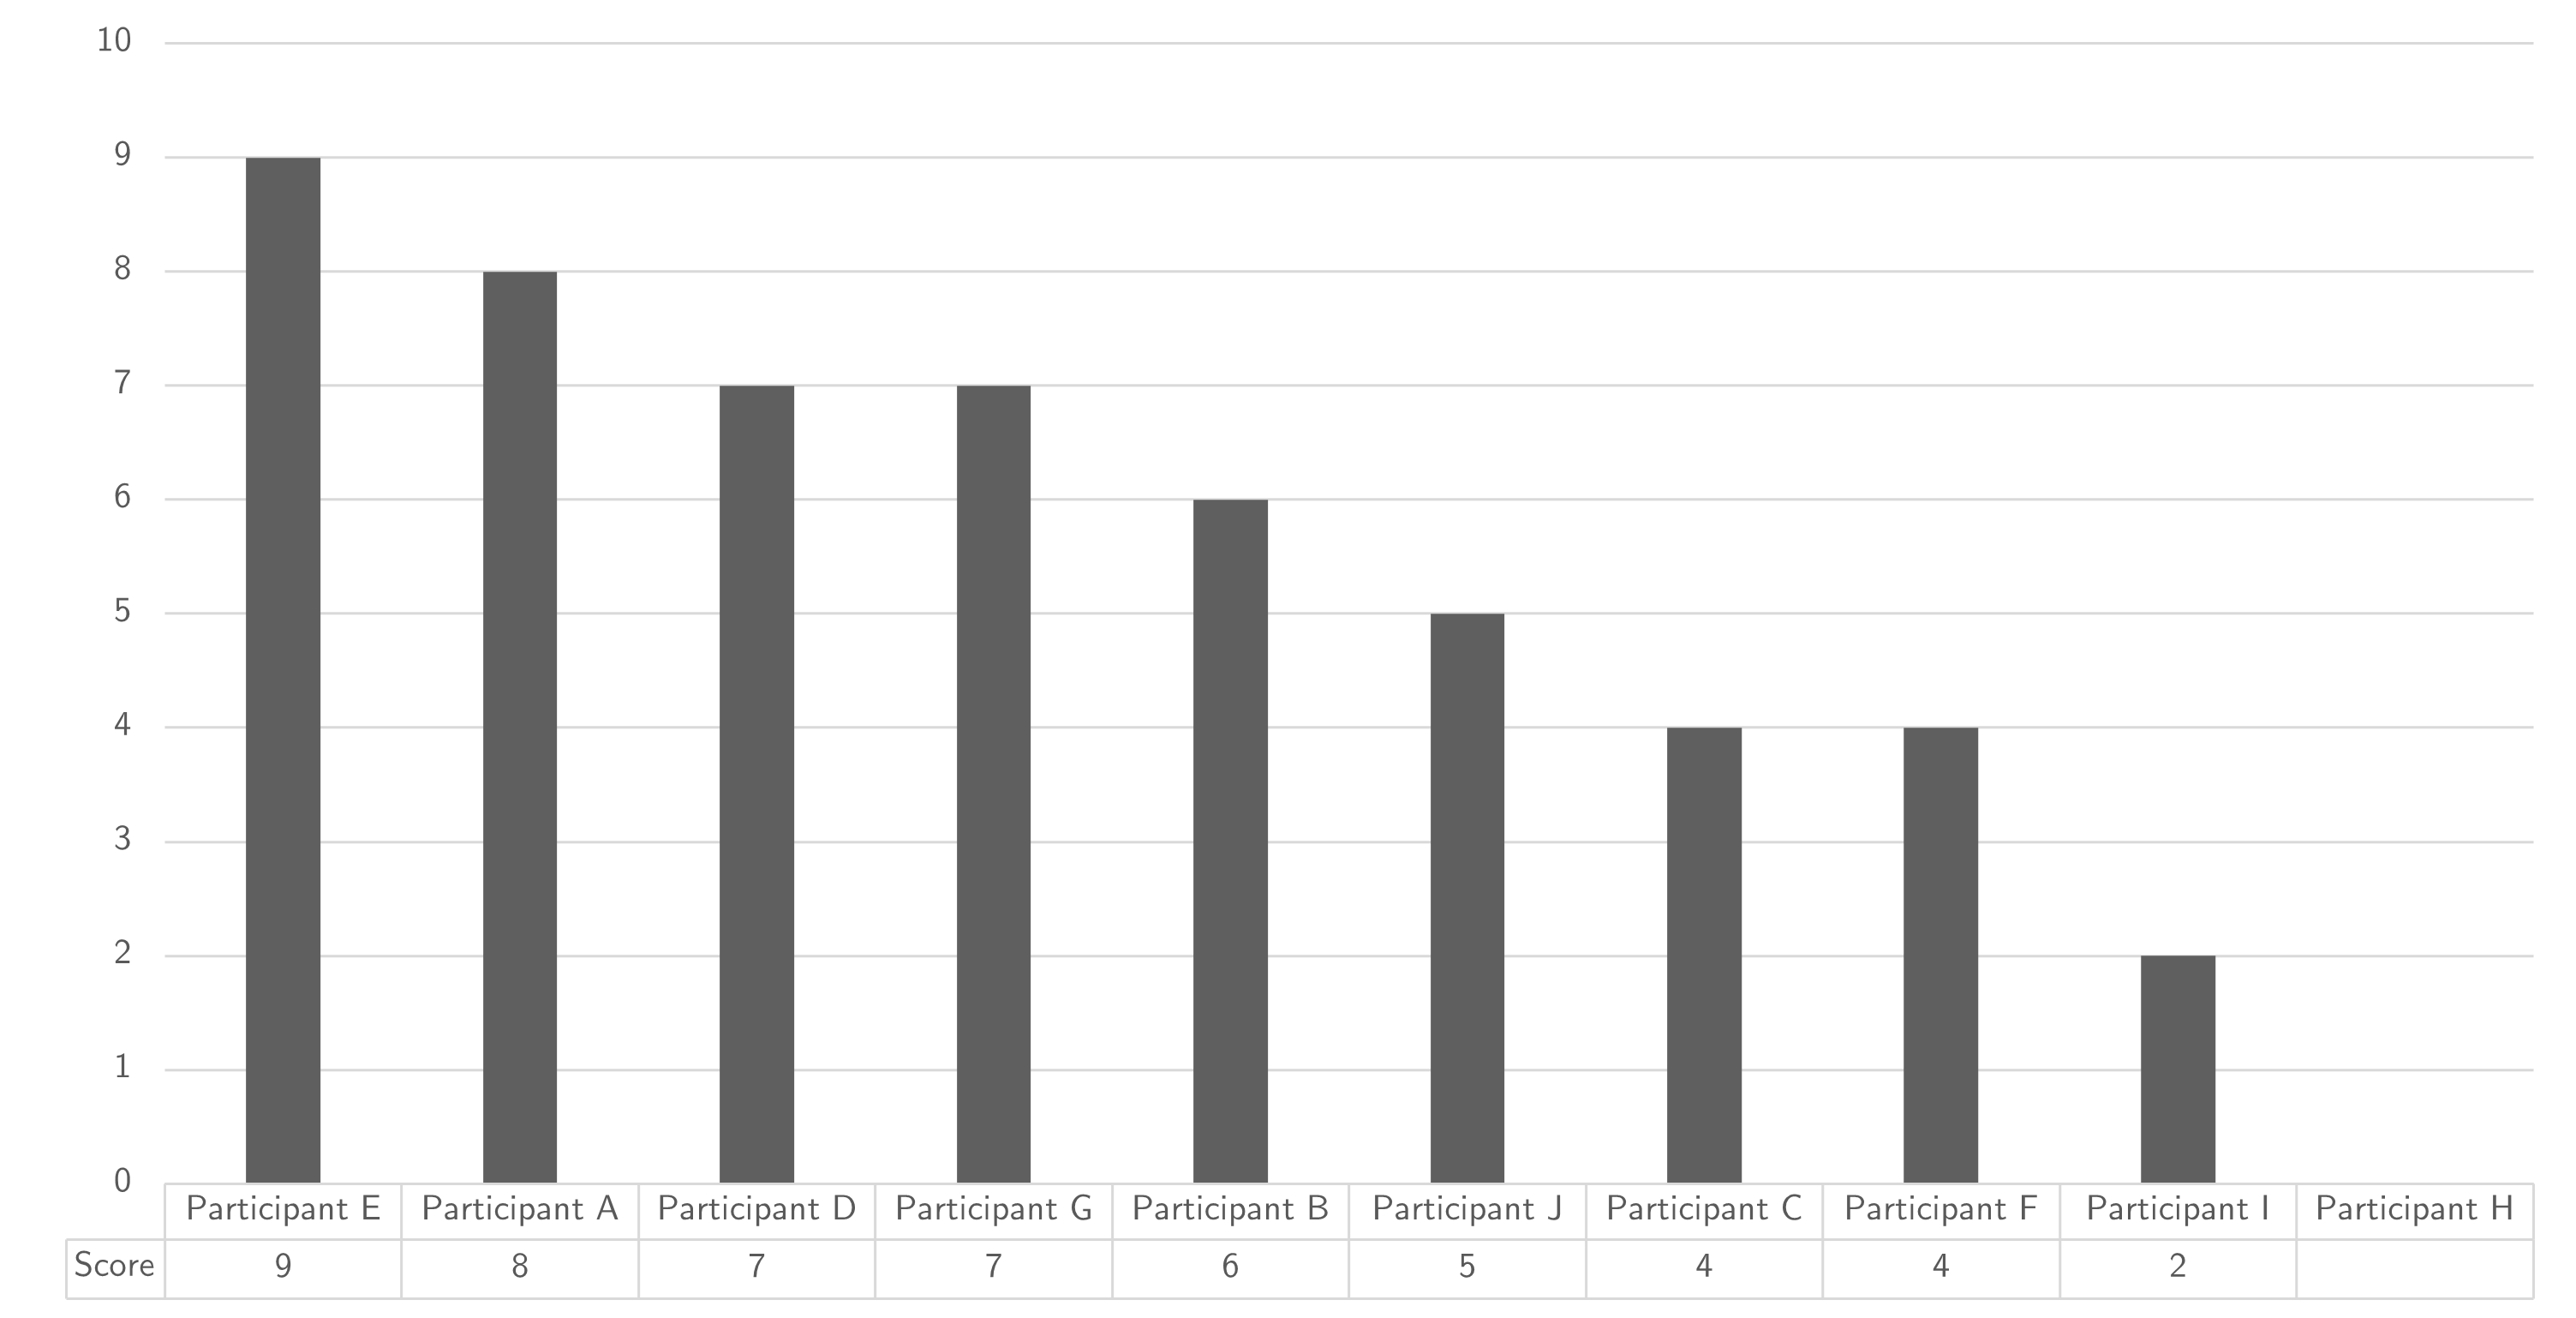
\includegraphics[width=0.9\linewidth]{images/scoreeaalwaysfitea}
	\caption[Scoring of EA attribute Always fitting EA]{Scoring of EA attribute Always fitting EA}
	\label{fig:appscoringeaalwaysfitea}
\end{figure}
\begin{table}[h!]
	\centering
	\begin{tabular}{p{.55\textwidth}ccc}
		\toprule
		\textbf{Attribute} & \textbf{Rating} & \textbf{Variability} & \textbf{Abstains} \\
		\midrule
		Always fitting EA & 5,8 & 46\% & 1 \\%
		\bottomrule
	\end{tabular}%
	\caption[Scoring of EA attribute Always fitting EA]{Scoring of EA attribute Always fitting EA}
	\label{tab:appscoringeaalwaysfitea}%
\end{table}%




\section{Closing Survey}
\begin{table}[!h]
	\centering
	\begin{tabular}{p{.55\textwidth}ccc}
		\toprule
		\textbf{Question} & \textbf{Rating} & \textbf{Variability} & \textbf{Abstains} \\
		\midrule
		To what extent do you find the research relevant? & 8,2 & 23\% & 0 \\%
		To what extent did this session fulfil your expectations? & 8 & 24\% & 0 \\%
		To what extent do you think that the research can be used by yourself? & 7,7 & 10\% & 0 \\%
		To what extent do you think that the research can be used in the public sector? & 7,2 & 32\% & 1 \\%
		To what extent do you think that the research can be used by your organisation? & 6,6 & 33\% & 0 \\%
		
		\bottomrule
	\end{tabular}%
	\caption{Closing Survey}
	\label{tab:appclosingsurvey}%
\end{table}%

\section{Follow-Up Survey}
\begin{table}[!h]
	\centering
	\begin{tabular}{p{.55\textwidth}ccc}
		\toprule
		\textbf{Question} & \textbf{Rating} & \textbf{Variability} & \textbf{Abstains} \\
		\midrule
		I want to receive possible updates on this research. & 9 & 0\% & 1 \\%
		I want to know when the thesis is published. & 9 & 0\% & 1 \\%
		\bottomrule
	\end{tabular}%
	\caption{Follow-up Survey}
	\label{tab:appfollowupsurvey}%
\end{table}%